%%%%%%%%%%%%%%%%%%%% book.tex %%%%%%%%%%%%%%%%%%%%%%%%%%%%%
%
% sample root file for the chapters of your "monograph"
%
% Use this file as a template for your own input.
%
%%%%%%%%%%%%%%%% Springer-Verlag %%%%%%%%%%%%%%%%%%%%%%%%%%


% RECOMMENDED %%%%%%%%%%%%%%%%%%%%%%%%%%%%%%%%%%%%%%%%%%%%%%%%%%%
\documentclass[graybox,envcountchap,a4paper]{svmono}

% choose options for [] as required from the list
% in the Reference Guide

%\usepackage{mathptmx}
%\usepackage{helvet}
%\usepackage{courier}
%

%% For language-specific hyphenations etc.
\usepackage[ngerman,english]{babel}
\usepackage[utf8]{inputenc} % Required for inputting international characters
\usepackage[T1]{fontenc} % Output font encoding for international characters
\usepackage{lmodern}
%% For subfigures
%\usepackage{subcaption}
%\captionsetup{compatibility=false}
% For nice links
\usepackage{url}
%Arbitrary size font selection 
\usepackage{type1cm}         
\usepackage{makeidx}         % allows index generation
\usepackage{graphicx}        % standard LaTeX graphics tool
% when including figure files
\graphicspath{{figures/}}
\usepackage{multicol}        % used for the two-column index
\usepackage[bottom]{footmisc}% places footnotes at page bottom

\usepackage{newtxtext}       % 
\usepackage{newtxmath}       % selects Times Roman as basic font

\usepackage{xcolor}

\usepackage{hyperref}
\hypersetup{
	pdftitle={Mining software development projects},
	pdfauthor={Saimir Bala},
	pdfkeywords={software development, business process management, visualisation, project mining},
	pdfsubject={mining software development projects},
	bookmarksopen=true,
	bookmarksopenlevel=0,
	hypertexnames=false,
	colorlinks=false,       % false: boxed links; true: colored links
	linkcolor=red,          % color of internal links (change box color with linkbordercolor)
	citecolor=green,        % color of links to bibliography
	filecolor=magenta,      % color of file links
	urlcolor=cyan,           % color of external links
	pdfstartview={FitV},
	unicode=true,
	breaklinks=true,
}

\urlstyle{same}

%% For playing with colors in tabular environments
%\usepackage{colortbl}

%% For math symbols, such as \nexists
%\usepackage{amssymb}
%% For more math symbols, such as \mapsfrom
%\usepackage{stmaryrd}
%%\usepackage{textcomp}
%% For advanced graphics
%%% For including figures, graphicx.sty has been loaded in
%%% elsarticle.cls. If you prefer to use the old commands
%%% please give \usepackage{epsfig}
%% For equations, arrays of equations, defining operator names, etc.
%\usepackage{amsmath}
%% For cursive math
%\usepackage{mathrsfs}
%% For math symbols, such as \nexists
%\usepackage{amssymb}
%%% For math environments, such as "definition"
%%\usepackage{amsthm}
%%\theoremstyle{definition}
%%\newdefinition{definition}{Definition}[section]
%%\newtheorem{theorem}{Theorem}[section]
%% For enumerating the line numbers
%\usepackage[left]{lineno}
%% For side notes, missing figures and inline to-do's
%\usepackage[textsize=scriptsize,backgroundcolor=orange!50]{todonotes}
%% For specifying kewords and acronyms
%\usepackage[nonumberlist,acronym,sanitize=none]{glossaries}
%\glsdisablehyper
%% For commenting out some parts of the text
%\usepackage{comment}
%%\usepackage{etoolbox}
%%\makeatletter
%%\patchcmd\@combinedblfloats{\box\@outputbox}{\unvbox\@outputbox}{}{%
%%	\errmessage{\noexpand\@combinedblfloats could not be patched}%
%%}%
%%\makeatother
%
%% For smart references
\usepackage{cleveref}
%% To have "Figure 3(a)" in place of "Figure 3a" and  "Table 3(a)" in place of "Table 3a"
%%\captionsetup[subfigure]{subrefformat=simple,labelformat=simple}
%%    \renewcommand\thesubfigure{(\alph{subfigure})}
%\captionsetup[subtable]{subrefformat=simple,labelformat=simple}
%    \renewcommand\thesubtable{(\alph{subtable})}
%\Crefname{algocf}{Algorithm}{Algorithms}
%% TikZ/Pgf advanced graphics
%\usepackage{tkz-base}
%\usetikzlibrary{decorations.pathmorphing,trees,snakes,arrows,shapes,automata}
%% To use inline and other fancy list-like environments (e.g., inparaenum)
%\usepackage{paralist}
%% To divide a text line into multiple columns
%\usepackage{multicol}
%% To create good-looking book-style tables
%\usepackage{booktabs}
%% To play around with list environments
%\usepackage{enumitem}
%% To create multirow cells in tables
%\usepackage{multirow}
%% To create rotated cells in tables
%\usepackage{rotating}
%%\usepackage{array}
%% To create enumerated lists, whose numbering is reversed
%\usepackage{etaremune}
%%% To make algorithmic nice-looking pseudocode
%\usepackage[ruled,linesnumbered]{algorithm2e}
%%% For creating side-notes
%% \usepackage{marginnote}
%% For superimposing symbols over one another within math env.
%\usepackage{mathtools}
%% For strange math symbols like \Dashv
%\usepackage{mathabx}
%% For LaTeX if/then statements
%\usepackage{ifthen}
%% For strike-through cancellations
%\usepackage[normalem]{ulem}
%%% The lineno packages adds line numbers. Start line numbering with
%%% \begin{linenumbers}, end it with \end{linenumbers}. Or switch it on
%%% for the whole article with \linenumbers.
%\usepackage{lineno}
%% For highlighted text
%\usepackage{soul}
%% To put table environments and co. side by side
%%\usepackage{floatrow}
%%\floatsetup[table]{style=plaintop}
%% To add dummy text
%\usepackage{lipsum}
%% To have newlines in cells, with commands such as \makecell or \thead
%\usepackage{makecell}
%% To enable text protrusion
%\usepackage{microtype}
%%\usepackage[showframe]{geometry}

%
%\AtBeginDocument{
%	\hypersetup{pdftitle=Mining software development projects} % Set the PDF's title to your title
%	\hypersetup{pdfauthor=Saimir Bala} % Set the PDF's author to your name
%	\hypersetup{pdfkeywords={software development, business process management, visualisation, project mining}} % Set the PDF's keywords to your keywords
%}


% see the list of further useful packages
% in the Reference Guide

\makeindex             % used for the subject index
                       % please use the style svind.ist with
                       % your makeindex program

%%%%%%%%%%%%%%%%%%%%%%%%%%%%%%%%%%%%%%%%%%%%%%%%%%%%%%%%%%%%%%%%%%%%%

\begin{document}

\author{Saimir Bala}
\title{Mining software development projects}
\subtitle{-- Monograph --}
%\maketitle

\frontmatter%%%%%%%%%%%%%%%%%%%%%%%%%%%%%%%%%%%%%%%%%%%%%%%%%%%%%%


%%%%%%%%%%%%%%%%%%%%%%% dedic.tex %%%%%%%%%%%%%%%%%%%%%%%%%%%%%%%%%
%
% sample dedication
%
% Use this file as a template for your own input.
%
%%%%%%%%%%%%%%%%%%%%%%%% Springer %%%%%%%%%%%%%%%%%%%%%%%%%%

\begin{dedication}
To Elias\\
\end{dedication}



 


\Extrachap{Abstract}

Here is an abstract



%%%%%%%%%%%%%%%%%%%%%%%foreword.tex%%%%%%%%%%%%%%%%%%%%%%%%%%%%%%%%%
% sample foreword
%
% Use this file as a template for your own input.
%
%%%%%%%%%%%%%%%%%%%%%%%% Springer %%%%%%%%%%%%%%%%%%%%%%%%%%

\foreword

%% Please have the foreword written here
Use the template \textit{foreword.tex} together with the document class SVMono (monograph-type books) or SVMult (edited books) to style your foreword\index{foreword}. 

The foreword covers introductory remarks preceding the text of a book that are written by a \textit{person other than the author or editor} of the book. If applicable, the foreword precedes the preface which is written by the author or editor of the book.


\vspace{\baselineskip}
\begin{flushright}\noindent
Place, month year\hfill {\it Firstname  Surname}\\
\end{flushright}



%%%%%%%%%%%%%%%%%%%%%%%preface.tex%%%%%%%%%%%%%%%%%%%%%%%%%%%%%%%%%%%%%%%%%
% sample preface
%
% Use this file as a template for your own input.
%
%%%%%%%%%%%%%%%%%%%%%%%% Springer %%%%%%%%%%%%%%%%%%%%%%%%%%

\preface

%% Please write your preface here
Use the template \emph{preface.tex} together with the document class SVMono (monograph-type books) or SVMult (edited books) to style your preface.

A preface\index{preface} is a book's preliminary statement, usually written by the \textit{author or editor} of a work, which states its origin, scope, purpose, plan, and intended audience, and which sometimes includes afterthoughts and acknowledgments of assistance. 

When written by a person other than the author, it is called a foreword. The preface or foreword is distinct from the introduction, which deals with the subject of the work.

Customarily \textit{acknowledgments} are included as last part of the preface.
 

\vspace{\baselineskip}
\begin{flushright}\noindent
Place(s),\hfill {\it Firstname  Surname}\\
month year\hfill {\it Firstname  Surname}\\
\end{flushright}



%%%%%%%%%%%%%%%%%%%%%%acknow.tex%%%%%%%%%%%%%%%%%%%%%%%%%%%%%%%%%%%%%%%%%
% sample acknowledgement chapter
%
% Use this file as a template for your own input.
%
%%%%%%%%%%%%%%%%%%%%%%%% Springer %%%%%%%%%%%%%%%%%%%%%%%%%%

\extrachap{Acknowledgements}

%Thanks to Jan, to the team, and many other people who I met along my PhD journey. They were all fundamental to shape my current self. The list is quite long.

Thanks to Jan, 
Claudio,
Cristina,
Andreas,
Johannes,
Giray, 
the rest of the team

Thanks to the Ski Seminars

Thanks to the guests who have visited the team with whom I had inspiring chats

Thanks to my co-authors.

Thanks to our project partners.

Last but not least, thanks to family. Kate.



\tableofcontents

\listoffigures

\listoftables

%%%%%%%%%%%%%%%%%%%%%%acronym.tex%%%%%%%%%%%%%%%%%%%%%%%%%%%%%%%%%%%%%%%%%
% sample list of acronyms
%
% Use this file as a template for your own input.
%
%%%%%%%%%%%%%%%%%%%%%%%% Springer %%%%%%%%%%%%%%%%%%%%%%%%%%

%\extrachap{Acronyms}
%

\setglossarypreamble[acronym]{List of abbreviations used in this thesis.}

%List of abbreviations used in this thesis.

%\begin{description}[CABR]
%\item[BPM]{Business Process Management}
%\item[XES]{eXtensible Event Stream}
%%\item[CABR]{Spelled-out abbreviation and definition}
%\end{description}

%\glsaddall
\setglossarystyle{long}
\setlength\LTleft{0pt}
\setlength\LTright{0pt}
\setlength\glsdescwidth{0.8\hsize}
\renewcommand{\glsnamefont}[1]{\textbf{#1}}
\printglossary[type=\acronymtype]

\mainmatter%%%%%%%%%%%%%%%%%%%%%%%%%%%%%%%%%%%%%%%%%%%%%%%%%%%%%%%
%\include{part}

%%%%%%%%%%%%%%%%%%%%%% chapter.tex %%%%%%%%%%%%%%%%%%%%%%%%%%%%%%%%%
%
% sample chapter
%
% Use this file as a template for your own input.
%
%%%%%%%%%%%%%%%%%%%%%%%% Springer-Verlag %%%%%%%%%%%%%%%%%%%%%%%%%%
%\motto{Use the template \emph{chapter.tex} to style the various elements of your chapter content.}
\chapter{Chapter Heading}
\label{intro} % Always give a unique label
% use \chaptermark{}
% to alter or adjust the chapter heading in the running head

\abstract*{Each chapter should be preceded by an abstract (no more than 200 words) that summarizes the content. The abstract will appear \textit{online} at \url{www.SpringerLink.com} and be available with unrestricted access. This allows unregistered users to read the abstract as a teaser for the complete chapter.
Please use the 'starred' version of the new \texttt{abstract} command for typesetting the text of the online abstracts (cf. source file of this chapter template \texttt{abstract}) and include them with the source files of your manuscript. Use the plain \texttt{abstract} command if the abstract is also to appear in the printed version of the book.}

\abstract{Each chapter should be preceded by an abstract (no more than 200 words) that summarizes the content. The abstract will appear \textit{online} at \url{www.SpringerLink.com} and be available with unrestricted access. This allows unregistered users to read the abstract as a teaser for the complete chapter. \newline\indent
Please use the 'starred' version of the new \texttt{abstract} command for typesetting the text of the online abstracts (cf. source file of this chapter template \texttt{abstract}) and include them with the source files of your manuscript. Use the plain \texttt{abstract} command if the abstract is also to appear in the printed version of the book.}

\section{Section Heading}
\label{sec:1}
Use the template \emph{chapter.tex} together with the document class SVMono (monograph-type books) or SVMult (edited books) to style the various elements of your chapter content conformable to the Springer Nature layout.

\section{Section Heading}
\label{sec:2}
% Always give a unique label
% and use \ref{<label>} for cross-references
% and \cite{<label>} for bibliographic references
% use \sectionmark{}
% to alter or adjust the section heading in the running head
Instead of simply listing headings of different levels we recommend to let every heading be followed by at least a short passage of text. Furtheron please use the \LaTeX\ automatism for all your cross-references and citations.

Please note that the first line of text that follows a heading is not indented, whereas the first lines of all subsequent paragraphs are.

\eject

Use the standard \verb|equation| environment to typeset your equations, e.g.
%
\begin{equation}
a \times b = c\;,
\end{equation}
%
however, for multiline equations we recommend to use the \verb|eqnarray| environment\footnote{In physics texts please activate the class option \texttt{vecphys} to depict your vectors in \textbf{\itshape boldface-italic} type - as is customary for a wide range of physical subjects.}.
\begin{eqnarray}
\left|\nabla U_{\alpha}^{\mu}(y)\right| &\le&\frac1{d-\alpha}\int
\left|\nabla\frac1{|\xi-y|^{d-\alpha}}\right|\,d\mu(\xi) =
\int \frac1{|\xi-y|^{d-\alpha+1}} \,d\mu(\xi)\qquad  \\
&=&(d-\alpha+1) \int\limits_{d(y)}^\infty
\frac{\mu(B(y,r))}{r^{d-\alpha+2}}\,dr \le (d-\alpha+1)
\int\limits_{d(y)}^\infty \frac{r^{d-\alpha}}{r^{d-\alpha+2}}\,dr
\label{eq:01}
\end{eqnarray}

\enlargethispage{24pt}

\subsection{Subsection Heading}
\label{subsec:2}
Instead of simply listing headings of different levels we recommend to let every heading be followed by at least a short passage of text. Further on please use the \LaTeX\ automatism for all your cross-references\index{cross-references} and citations\index{citations} as has already been described in Sect.~\ref{sec:2}.

\begin{quotation}
Please do not use quotation marks when quoting texts! Simply use the \verb|quotation| environment -- it will automatically be rendered in the preferred layout.
\end{quotation}


\subsubsection{Subsubsection Heading}
Instead of simply listing headings of different levels we recommend to let every heading be followed by at least a short passage of text. Furtheron please use the \LaTeX\ automatism for all your cross-references and citations as has already been described in Sect.~\ref{subsec:2}, see also Fig.~\ref{fig:1}\footnote{If you copy text passages, figures, or tables from other works, you must obtain \textit{permission} from the copyright holder (usually the original publisher). Please enclose the signed permission with the manucript. The sources\index{permission to print} must be acknowledged either in the captions, as footnotes or in a separate section of the book.}

Please note that the first line of text that follows a heading is not indented, whereas the first lines of all subsequent paragraphs are.

% For figures use
%
\begin{figure}[b]
\sidecaption
% Use the relevant command for your figure-insertion program
% to insert the figure file.
% For example, with the option graphics use
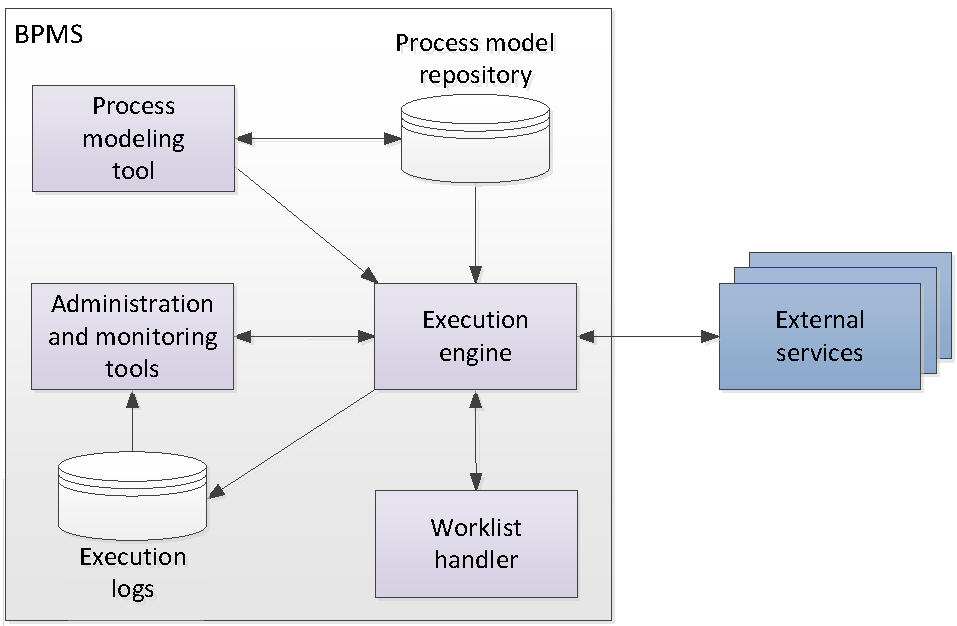
\includegraphics[scale=.65]{figure}
%
% If not, use
%\picplace{5cm}{2cm} % Give the correct figure height and width in cm
%
\caption{If the width of the figure is less than 7.8 cm use the \texttt{sidecapion} command to flush the caption on the left side of the page. If the figure is positioned at the top of the page, align the sidecaption with the top of the figure -- to achieve this you simply need to use the optional argument \texttt{[t]} with the \texttt{sidecaption} command}
\label{fig:1}       % Give a unique label
\end{figure}


\paragraph{Paragraph Heading} %
Instead of simply listing headings of different levels we recommend to let every heading be followed by at least a short passage of text. Furtheron please use the \LaTeX\ automatism for all your cross-references and citations as has already been described in Sect.~\ref{sec:2}.

Please note that the first line of text that follows a heading is not indented, whereas the first lines of all subsequent paragraphs are.

For typesetting numbered lists we recommend to use the \verb|enumerate| environment -- it will automatically render Springer's preferred layout.

\begin{enumerate}
\item{Livelihood and survival mobility are oftentimes coutcomes of uneven socioeconomic development.}
\begin{enumerate}
\item{Livelihood and survival mobility are oftentimes coutcomes of uneven socioeconomic development.}
\item{Livelihood and survival mobility are oftentimes coutcomes of uneven socioeconomic development.}
\end{enumerate}
\item{Livelihood and survival mobility are oftentimes coutcomes of uneven socioeconomic development.}
\end{enumerate}


\subparagraph{Subparagraph Heading} In order to avoid simply listing headings of different levels we recommend to let every heading be followed by at least a short passage of text. Use the \LaTeX\ automatism for all your cross-references and citations as has already been described in Sect.~\ref{sec:2}, see also Fig.~\ref{fig:2}.

Please note that the first line of text that follows a heading is not indented, whereas the first lines of all subsequent paragraphs are.

For unnumbered list we recommend to use the \verb|itemize| environment -- it will automatically render Springer's preferred layout.

\begin{itemize}
\item{Livelihood and survival mobility are oftentimes coutcomes of uneven socioeconomic development, cf. Table~\ref{tab:1}.}
\begin{itemize}
\item{Livelihood and survival mobility are oftentimes coutcomes of uneven socioeconomic development.}
\item{Livelihood and survival mobility are oftentimes coutcomes of uneven socioeconomic development.}
\end{itemize}
\item{Livelihood and survival mobility are oftentimes coutcomes of uneven socioeconomic development.}
\end{itemize}

\begin{figure}[t]
\sidecaption[t]
% Use the relevant command for your figure-insertion program
% to insert the figure file.
% For example, with the option graphics use
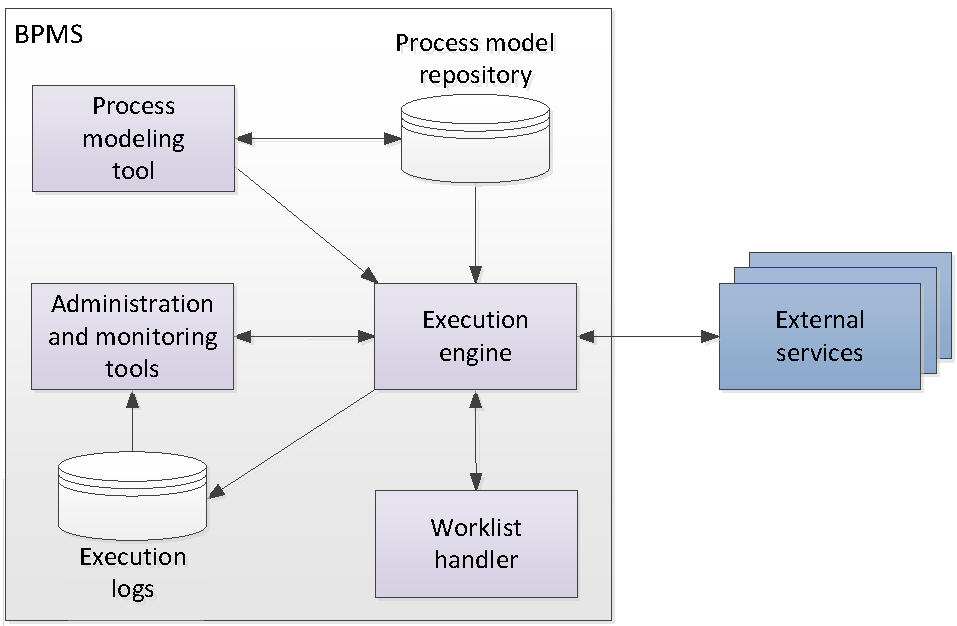
\includegraphics[scale=.65]{figure}
%
% If not, use
%\picplace{5cm}{2cm} % Give the correct figure height and width in cm
%
\caption{Please write your figure caption here}
\label{fig:2}       % Give a unique label
\end{figure}

\runinhead{Run-in Heading Boldface Version} Use the \LaTeX\ automatism for all your cross-references and citations as has already been described in Sect.~\ref{sec:2}.

\subruninhead{Run-in Heading Boldface and Italic Version} Use the \LaTeX\ automatism for all your cross-refer\-ences and citations as has already been described in Sect.~\ref{sec:2}\index{paragraph}.

\subsubruninhead{Run-in Heading Displayed Version} Use the \LaTeX\ automatism for all your cross-refer\-ences and citations as has already been described in Sect.~\ref{sec:2}\index{paragraph}.
% Use the \index{} command to code your index words
%
% For tables use
%
\begin{table}
\caption{Please write your table caption here}
\label{tab:1}       % Give a unique label
%
% For LaTeX tables use
%
\begin{tabular}{p{2cm}p{2.4cm}p{2cm}p{4.9cm}}
\hline\noalign{\smallskip}
Classes & Subclass & Length & Action Mechanism  \\
\noalign{\smallskip}\svhline\noalign{\smallskip}
Translation & mRNA$^a$  & 22 (19--25) & Translation repression, mRNA cleavage\\
Translation & mRNA cleavage & 21 & mRNA cleavage\\
Translation & mRNA  & 21--22 & mRNA cleavage\\
Translation & mRNA  & 24--26 & Histone and DNA Modification\\
\noalign{\smallskip}\hline\noalign{\smallskip}
\end{tabular}
$^a$ Table foot note (with superscript)
\end{table}
%
\section{Section Heading}
\label{sec:3}
% Always give a unique label
% and use \ref{<label>} for cross-references
% and \cite{<label>} for bibliographic references
% use \sectionmark{}
% to alter or adjust the section heading in the running head
Instead of simply listing headings of different levels we recommend to let every heading be followed by at least a short passage of text. Furtheron please use the \LaTeX\ automatism for all your cross-references and citations as has already been described in Sect.~\ref{sec:2}.

Please note that the first line of text that follows a heading is not indented, whereas the first lines of all subsequent paragraphs are.

If you want to list definitions or the like we recommend to use the Springer-enhanced \verb|description| environment -- it will automatically render Springer's preferred layout.

\begin{description}[Type 1]
\item[Type 1]{That addresses central themes pertainng to migration, health, and disease. In Sect.~\ref{sec:1}, Wilson discusses the role of human migration in infectious disease distributions and patterns.}
\item[Type 2]{That addresses central themes pertainng to migration, health, and disease. In Sect.~\ref{subsec:2}, Wilson discusses the role of human migration in infectious disease distributions and patterns.}
\end{description}

\subsection{Subsection Heading} %
In order to avoid simply listing headings of different levels we recommend to let every heading be followed by at least a short passage of text. Use the \LaTeX\ automatism for all your cross-references and citations citations as has already been described in Sect.~\ref{sec:2}.

Please note that the first line of text that follows a heading is not indented, whereas the first lines of all subsequent paragraphs are.

\begin{svgraybox}
If you want to emphasize complete paragraphs of texts we recommend to use the newly defined Springer class option \verb|graybox| and the newly defined environment \verb|svgraybox|. This will produce a 15 percent screened box 'behind' your text.

If you want to emphasize complete paragraphs of texts we recommend to use the newly defined Springer class option and environment \verb|svgraybox|. This will produce a 15 percent screened box 'behind' your text.
\end{svgraybox}


\subsubsection{Subsubsection Heading}
Instead of simply listing headings of different levels we recommend to let every heading be followed by at least a short passage of text. Furtheron please use the \LaTeX\ automatism for all your cross-references and citations as has already been described in Sect.~\ref{sec:2}.

Please note that the first line of text that follows a heading is not indented, whereas the first lines of all subsequent paragraphs are.

\begin{theorem}
Theorem text goes here.
\end{theorem}
%
% or
%
\begin{definition}
Definition text goes here.
\end{definition}

\begin{proof}
%\smartqed
Proof text goes here.
%\qed
\end{proof}

\paragraph{Paragraph Heading} %
Instead of simply listing headings of different levels we recommend to let every heading be followed by at least a short passage of text. Furtheron please use the \LaTeX\ automatism for all your cross-references and citations as has already been described in Sect.~\ref{sec:2}.

Note that the first line of text that follows a heading is not indented, whereas the first lines of all subsequent paragraphs are.
%
% For built-in environments use
%
\begin{theorem}
Theorem text goes here.
\end{theorem}
%
\begin{definition}
Definition text goes here.
\end{definition}
%
\begin{proof}
%\smartqed
Proof text goes here.
%\qed
\end{proof}
%
%
\begin{trailer}{Trailer Head}
If you want to emphasize complete paragraphs of texts in an \verb|Trailer Head| we recommend to
use  \begin{verbatim}\begin{trailer}{Trailer Head}
...
\end{trailer}\end{verbatim}
\end{trailer}
%
\begin{example}{Example}
If you want to emphasize complete paragraphs of texts in an \verb|Example| we recommend to
use  \begin{verbatim}\begin{example}{Example}
...
\end{example}\end{verbatim}
\end{example}
%
\begin{question}{Questions}
If you want to emphasize complete paragraphs of texts in an \verb|Questions| we recommend to
use  \begin{verbatim}\begin{question}{Questions}
...
\end{question}\end{verbatim}
\end{question}
%
\clearpage
%
\begin{important}{Important}
If you want to emphasize complete paragraphs of texts in an \verb|Important| we recommend to
use  \begin{verbatim}\begin{important}{Important}
...
\end{important}\end{verbatim}
\end{important}
%
\begin{warning}{Attention}
If you want to emphasize complete paragraphs of texts in an \verb|Attention| we recommend to
use  \begin{verbatim}\begin{warning}{Attention}
...
\end{warning}\end{verbatim}
\end{warning}

\begin{programcode}{Program Code}
If you want to emphasize complete paragraphs of texts in an \verb|Program Code| we recommend to
use

\verb|\begin{programcode}{Program Code}|

\verb|\begin{verbatim}...\end{verbatim}|

\verb|\end{programcode}|

\end{programcode}
%
\begin{tips}{Tips}
If you want to emphasize complete paragraphs of texts in an \verb|Tips| we recommend to
use  \begin{verbatim}\begin{tips}{Tips}
...
\end{tips}\end{verbatim}
\end{tips}
%
\clearpage
%
\begin{overview}{Overview}
If you want to emphasize complete paragraphs of texts in an \verb|Overview| we recommend to
use  \begin{verbatim}\begin{overview}{Overview}
...
\end{overview}\end{verbatim}
\end{overview}
\begin{backgroundinformation}{Background Information}
If you want to emphasize complete paragraphs of texts in an \verb|Background|
\verb|Information| we recommend to
use

\verb|\begin{backgroundinformation}{Background Information}|

\verb|...|

\verb|\end{backgroundinformation}|
\end{backgroundinformation}
\begin{legaltext}{Legal Text}
If you want to emphasize complete paragraphs of texts in an \verb|Legal Text| we recommend to
use  \begin{verbatim}\begin{legaltext}{Legal Text}
...
\end{legaltext}\end{verbatim}
\end{legaltext}
%
\begin{acknowledgement}
If you want to include acknowledgments of assistance and the like at the end of an individual chapter please use the \verb|acknowledgement| environment -- it will automatically render Springer's preferred layout.
\end{acknowledgement}
%
\section*{Appendix}
\addcontentsline{toc}{section}{Appendix}
%
When placed at the end of a chapter or contribution (as opposed to at the end of the book), the numbering of tables, figures, and equations in the appendix section continues on from that in the main text. Hence please \textit{do not} use the \verb|appendix| command when writing an appendix at the end of your chapter or contribution. If there is only one the appendix is designated ``Appendix'', or ``Appendix 1'', or ``Appendix 2'', etc. if there is more than one.

\begin{equation}
a \times b = c
\end{equation}
% Problems or Exercises should be sorted chapterwise
\section*{Problems}
\addcontentsline{toc}{section}{Problems}
%
% Use the following environment.
% Don't forget to label each problem;
% the label is needed for the solutions' environment
\begin{prob}
\label{prob1}
A given problem or Excercise is described here. The
problem is described here. The problem is described here.
\end{prob}

\begin{prob}
\label{prob2}
\textbf{Problem Heading}\\
(a) The first part of the problem is described here.\\
(b) The second part of the problem is described here.
\end{prob}



\chapter{Introduction}
\label{chap:intro} % Always give a unique label
% use \chaptermark{}
% to alter or adjust the chapter heading in the running head

This chapter provides an introduction to this doctoral thesis. \Cref{sec:intro-motivation} motivates the research. \Cref{sec:problem-definition} defines the problem. \Cref{sec:intro-research-paradigm} gives an overview of the research methodology and defines the artifacts generated as outcome. \Cref{sec:data-collection} briefly discusses the data created and used in this thesis. \Cref{sec:intro-contributions} classifies the contributions of this thesis. \Cref{sec:intro-structure} provides an outlook of the structure, and \Cref{sec:intro-related-publications} lists the publications that have resulted from work on this thesis. 

\section{Motivation}
\label{sec:intro-motivation}

Software development is a process that involves creativity (\citealp{DBLP:journals/jss/AldaveVGM19,DBLP:journals/jss/DingsoyrNBM12}). Yet, practical software development projects are executed with specific requirements on time, budget and quality. In order to fulfill these requirements the development process must be monitored. For example, it is important to know what type of work is being done at a certain moment in time and by whom. This is for instance the case for large development projects where coordination mechanisms emerge spontaneously among developers who want to contribute with their code.
These type of projects are difficult to control for several reasons. First, there is no clear understanding in how far a certain piece of code advances the current status of the project. Second, a piece of code written by a developer goes through different stages of code-review and it is difficult to predict whether it will ever be merged with the main source. Third, coordination of work may involve a large number of message exchanges among many developers in forums. Hence, it is not feasible to manually oversee what work is going on at a particular point in time. 

Literature has tackled this problem from different angles. In the area of process mining approaches exist that exploit event logs for abstracting a process model. In the area of software engineering, software repositories have been the major interest. Contributions from this area provide several metrics that help with understanding various aspects of development. However, process mining approaches only work with event logs where activities are explicitly recorded in the log. This is not the case with software development where data is rather unstructured. Likewise, software engineering approaches lack a perspective about work patterns. 


This study addresses the discovery of work patterns from software development event data. To this end, it defines concepts to capture work from software repositories. This allows to construct several discovery techniques that provide information about different perspectives of the development process. More specifically we categorize them into \emph{time}, \emph{case}, \emph{organizational} and \emph{control-flow}. The time perspective informs about temporal aspects of the process, such as when did an activity happen and for how long. The case perspective informs about characteristic of the different cases, such as the number of lines of code being produced at during the creation of each version of an artifact. The organizational perspective informs about the roles of the people in the context of the organization, such as developers, testers, etc. The control-flow perspective informs about the logical succession of activities, such as an artifact must first be implemented and then tested. 

In this sense, this work provides a bridge between process mining and software engineering. The findings of this work enable project managers as well as software developers to raise transparency about the actual development based on facts. As a result, it enables both understanding the current status and monitoring for potentially unwanted patterns of work.

%The rest of this proposal is organized as follows. \Cref{sec:problem-definition} describes the problem, the existing literature, and derives the solution requirements. \Cref{sec:state-of-field} provides background knowledge on the related fields of process mining, text mining, and mining software repositories. \Cref{sec:methods} explains the research method, the dataset and outlines the expected output of the thesis. \Cref{sec:preliminary-results} shows completed work so far. \Cref{sec:next-steps} outlines future steps towards the completion of this dissertation. \Cref{sec:dissertation-relevance} draws the implications for research and presents a dissemination plan.


\section{Problem Definition}
\label{sec:problem-definition}

%\todo[inline]{Here, too, include the four perspectives. Fig.1. can change: "4-perspectives of work" and include time, orga, control-flow, case. Include citations.}

%\todo[inline]{Check overlap of information provided here versus info provided in the background section. E.g. details of VCS.}

Software development processes are highly complex endeavors that require the coordination of multiple resources. Compared to standard business processes, they present the following characteristics. First, 
%although there is a planning phase, 
they involve creativity when executing the tasks, i.e. there exists no strict process model that is followed by the developers to produce a new piece of code. Second, they are driven by methodologies, e.g., \gls{rup}, Scrum\footnote{\url{https://www.scrum.org}}, Waterfall, etc. These methodologies constitute guidelines and best practices for project success. Third, they typically make use of software tools such as \gls{its} \index{its}, \gls{vcs} \index{version control system} and \gls{ide} \index{integrated development environment}. Such tools typically record work activities into log files. Fourth, there is in general no process engine to control the execution. Rather than that, a project manager or a Scrum master has to make sure that tasks are made available to the respective resources. Fifth, it is not trivial to obtain high level information on performance measures such as the burn-down rate, which are resource bottlenecks, what are time requirements for certain tasks, what type of work is actually being done, and how productive are people working in certain tasks, etc. Hence, there is the need for algorithms and tools that help extracting this knowledge.

\begin{figure}
	\centering
	
\includegraphics[width=0.4\linewidth]{figures/data-to-work}
	\caption{Automatically derive work from trace data}
	\label{fig:data-to-work}
\end{figure}


Software development processes fall into the category of \emph{project-oriented business processes} \citep{DBLP:conf/bpm/BalaCMRP15}. 
That is, they are rather ad-hoc plans performed with limited resources and time, but with a clear goal: develop a software artifact. Unlike classic business processes which are best captured with notations such as Petri nets and \gls{bpmn}, software development processes are more akin to one-time plans, which are usually captured by models such as Gantt and PERT diagrams. The following example captures the essence of a typical software development process in practice, such as for instance in Google LLC \citep{Henderson2017}.


\begin{quote}
	A new software version or feature needs to be developed. Unquestionably, Google has know-how on software development. However, before starting the implementation phase, precise requirements for tasks must be formulated. These tasks are stored in \gls{its} and referred to as \emph{issues}. Usually effort estimation values are assigned to each of them. Subsequently time and resources are allocated to the tasks. This starts the implementation phase. During this phase, resources work on tasks in a creative way, choosing among available tasks according to their own skills and expertise. In order to save the progress, developers issue a so-called \emph{commit} command which creates a new version of the modified files on the \gls{vcs}. Likewise, every time a certain task (which may be carried out through by different commits) is completed, the corresponding issue is marked as done. Both commits and issues can be commented by the users, respectively to document the changes and raise a discussion for increasing understanding the problem.
\end{quote}

Several tools are used by software project participants to support their work. Therefore, traces about the overall process are typically available in different repositories and artifacts, e.g., spreadsheets, word processor documents, programming languages files, emails, etc. This makes it cumbersome to obtain knowledge about the overall business process through manual inspection. Also, it is a challenge to automatically \emph{extract} work information from unstructured data such as user comments when working on tasks. For instance, existing solutions (e.g., process mining algorithms) are not able to provide informative results when the data is not available as a structured single event log where activities are explicitly labeled. Likewise, other software tools (e.g. GitHub) limit themselves at providing only process-unaware statistical information (e.g., number of commits in a file).

%Therefore, the overall challenge is to understand which are important events that track development work in the repository. 


While obtaining an overarching view on software development is challenging, there are still repositories that can be exploited to obtain process knowledge. One tool that provides important traces of the development work is \gls{vcs}. This tool is used to keep track of the different versions of files created by users and to manage their collaboration. Not only supports it keeping track of file versions, but also allows users to associate a textual comment that describe the changes made. Therefore, a new version of a particular file is created as the result of an activity done by a user. The evolution of these versions, along with information about the users and their comments can be retrieved from these type of tools in the form of semi-structured event logs. It is then a challenge how to discover the business process from events (e.g., lines of code changed, comments, user information) present in these logs.

%
%\todo{JM: I think you have to develop much more clearly how it is difficult to extract certain pieces of information from version control systems.} 

%An important dimension of the software development process is the work dimension, i.e. the process. This perspective is particularly interesting to project managers. One of their goal is to know whether the planning phase was realistic with respect to the development efforts. Existing software repositories allow for many ways to access their log files. These log files offer factual information about actions done by the process participants to change the repository state.

\begin{figure}[h]
	\centering
	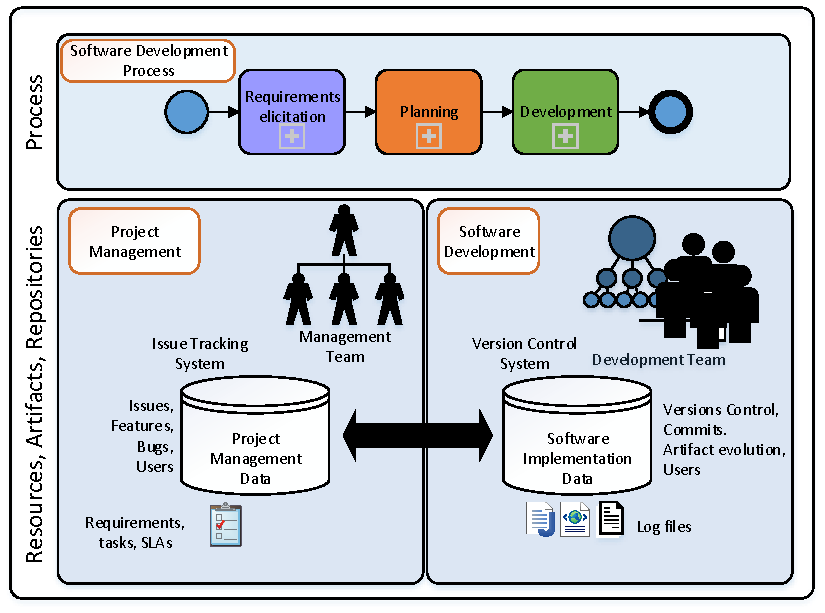
\includegraphics[width=\linewidth]{figures/big-picture}
	\caption{Software development scenario with two repositories used for project management and software development, respectively.}
	\label{fig:big-picture-sd}
\end{figure}

\Cref{fig:big-picture-sd} illustrates such problem scenario. Software development relies on tools like \gls{its} (e.g., JIRA, GitHub Issues) and \gls{vcs} (e.g. Subversion, Git). \Gls{its} is used for tracking the project management aspect. This aspect offers plan related information, such as issues, features, bugs, text, planned and executed tasks, timestamps, stories, and effort estimation (e.g., story points in JIRA).
\Gls{vcs} offers information about work traces, such as versions of the artifacts, number and content of commits done by developers, artifacts evolution, users and their comments, and timestamps of each action. 
% Please add the following required packages to your document preamble:
% \usepackage{booktabs}

% \usepackage[normalem]{ulem}
% \useunder{\uline}{\ul}{}
%\vspace*{-.5cm}
\newcommand{\rowsep}{\vspace*{2pt}}
%\newcommand{\colsep}{\hspace*{52pt}}
\begin{table}[h]
%	\small
	\caption{An excerpt of a VCS log data}
	\label{tab:vcs-log-data1}
	\setlength{\tabcolsep}{6pt}
%	\setlength\belowcaptionskip{-20pt}
\centering
%\resizebox{.99\textwidth}{!}{%
%\begin{tabular}{@{ }cm{.7cm}m{2cm}m{4.8cm}m{7cm}@{ }}
\begin{tabular}{@{~~}lm{1cm}m{1.4cm}m{1.7cm}m{5cm}@{~~}}
\toprule
\textbf{Id} & \textbf{Resource} & \textbf{Date}                          & \textbf{Comment}                          & \textbf{Diff}                                                                                                                                                                                                                                                                                   \\ \midrule 
%\rowcolor{lightgray}
1          & John    & 2017-01-31 12:16:30 & Create readme file                   & \begin{tabular}[c]{@{}l@{}}diff --git a/README.md b/README.md\\ @@ -0,0 +1 @@\\+\# StoryMiningSoftwareRepositories \end{tabular}                                                                                                                                                          \\ \rowcolor{lightgray}
\addlinespace
2          & Mary    & 2017-02-01 10:13:51 & Add a license                   &  \begin{tabular}[c]{@{}l@{}}diff --git a/README b/README\\ @@ -1,0 +2,3 @@\\ +The MIT License (MIT)\\ +\\ +Copyright (c) 2015 Mary+\end{tabular}                                                                                                                                     \\ \addlinespace
%\rowcolor{lightgray} 
3          & Paul    & 2017-02-02 16:10:22 & Updated the requirements.               &  \begin{tabular}[c]{@{}l@{}}diff --git a/README.md b/README.md\\ @@ -1,4 +1,5 @@ \\ + \# string 1, string 2, string 3\\ \\ diff --git a/requirements.txt b/requirements.txt\\ @@ -0,0 +1 @@\\ +The software must solve the problems\end{tabular} \\ \rowcolor{lightgray} \addlinespace

4          & Paul    & 2017-02-02 15:00:02 & Implement new requirements &  \begin{tabular}[c]{@{}l@{}}diff --git a/model.java b/model.java\\ @@ -1,9 +1,10 @@ \\ {+public static methodA()\{int newVal=0;}\\ @@ -21,10 +23,11 @@\\ + "1/0",,"0/0",\\ \\ diff --git a/test.java b/test.java\\ @@ -0,0 +1,2 @@\\ +//test method A\\ +testMethodA()\end{tabular}  \\ \bottomrule
\end{tabular}%
%}
\end{table} 


Although different technologies exist in practice (e.g., Subversion, Mercurial, Git), the information contained in the logs can be roughly summarized by \Cref{tab:vcs-log-data}. \todo{Maybe I can change this table with a more generic one that contains all information?}  The table displays an excerpt of a \gls{vcs} log, i.e., a set of user commits, after having extracted and structured the data according to five attributes. The semantics of the  attributes is a follows: 
\begin{inparaenum}[\itshape i)]
	\item \emph{Id} is a unique identifier;
	\item \emph{Resource} is the resource that issued the commit;
	\item \emph{Date} is a timestamp associated to the time and date the commit was stored in the system;
	\item \emph{Comment} is a user comment on the changes made;
	\item \emph{Diff} is low-level information on the difference between the current and the previous version, for each file.
\end{inparaenum} 
Likewise, information about issues from \gls{its} can be extracted and presented in a tabular way. In this case, other attributes are more important. These attributes can be, for example, the status of issues and the conversations that take place around them. %As the relation between \gls{its} and \gls{vcs} about requirements-implementation, we can narrow down our research question to the following. \emph{\textbf{RQ:} How does the specification of user stories influence software development work?} 
%In the more specific case, \gls{vcs} logs consist of an ordered set of \emph{commits} bearing information about users, files, timestamp, comments and type of change that were stored at particular moment in time. \Gls{its} typically come with richer information, most importantly they inform about users, task, type of task (e.g., bug, new feature, requirement, etc), timestamps, related issues, etc. 
%Many types of analyses can be performed on such feature rich data once they have been properly correlated and structured. 
Hence, studying the co-evolution of these two repositories can help extracting relevant knowledge about the software development process. 

More precisely this work seeks answer to the following research question. \textbf{RQ}: \emph{How can we make use of project event data to gather insights about the software development process that are informative to managers?} 
Because the project managers can benefit from a process view to better analyze hidden aspects of the software development process, this work takes a process mining stance on the problem. Therefore, the main research question is broken down into the following four subquestions. Each of them addresses \textbf{RQ} with respect to the four perspectives of a process that are useful to discover the event data \citep{VanderAalst2016b}.

%In the light of the above considerations, we derive the following requirements for extending process mining towards the analysis of software repositories.
%Owing to \gls{pm} literature, the research question (\textbf{RQ}) can be further broken down to the four process mining perspectives. 
%From here, we derive the four fundamental requirements that satisfy \gls{msd}.

\begin{inparadesc}
	\item[RQ1.] \emph{How can we use project event data to extract information about the \textbf{temporal} perspective of activities?} 
	%	For example, an answer to this question would look like: the development activity has a duration of 2 weeks on average, the average time of task creation is 15 minutes, etc. 
	
	\item[RQ2.] \emph{How can we use project event data to extract information about the \textbf{case} perspective?} 
	%	For example, an answer to this question would look like: all the bugs are solved in a 3 steps iteration, or a quality piece of code takes a conversation with 3 people and is successfully merged into the main branch after 1 week, etc.
	
	\item[RQ3.] \emph{How can we use project event data to extract information about the \textbf{organizational} perspective?} 
	%	For example, an answer to this question would look like: the software development is carried out by a team of 4 people, the actual user roles in the company are developer and tester, etc.
	
	\item[RQ4.] \emph{How can we use project event data to extract information about the \textbf{control-flow} perspective?} 
	%	For example, an answer to this question would look like: the testing is always done before development, or while new features are worked on, also new requirements are created, etc. Note that, differently from \textbf{RQ1} this question focuses on the logical connection and order of activities.
	
\end{inparadesc}

\section{Research Methodology and Generated Artifacts}
\label{sec:intro-research-paradigm}

%\todo[inline]{Here goes Peffers \citep{Peffers2008}
%	
%	Make clear what type of contribution you are proposing. E.g., engineering: set of techniques, algorithms, etc.
%	
%	This section presents the research method. It also describes the dataset and outlines the expected research outcome.
%}

This thesis is positioned as design science \citep{Hevner2004}.
Information systems research is an interdisciplinary field of study that uses theories from social sciences, economics, and computer science. The field can be divided into two complementary paradigms: \emph{behavioral science} and \emph{design science}. Behavioral science aims at developing and justifying theories in order to explain or predict information systems phenomena \cite[]{Gregor2006}. Design science focuses on the creation and evaluation of innovative design \emph{artifacts} \cite[]{Hevner2004}. \Cref{fig:DS-process} illustrates the design science approach as a process \citep{Peffers2008}. 

\begin{figure}[h]
	\centering
	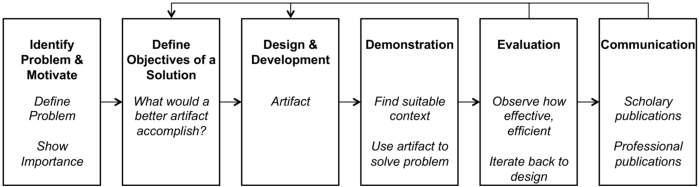
\includegraphics[width=\linewidth]{figures/DS-process}
	\caption[The Design Science Research process]{The Design Science Research process, adapted from \citep{Peffers2008}}
	\label{fig:DS-process}
\end{figure}

%This doctoral thesis employs both design and behavioral science. Following the approach suggested by \cite[]{Berente2018}, real life data will be used for data-driven computationally-intensive theory development. \todoinline{JM: You really want to develop theory, or you aim to provide techniques? I think you work is more about providing technique - that are useful to inform the mentioned approach to theory building.} This approach can be seen as a combination between behavioral science and design science. The behavioral perspective is given by traditional theory development based on manual coding, e.g. \gls{gtm}. The design perspective is given by the creation of novel artifacts (e.g., software algorithms) that use trace data to automatically discover theory, e.g, \gls{ctd}. This thesis uses real world data gathered from the SHAPE project\footnote{\url{https://aic.ai.wu.ac.at/shape-project/}} and \gls{oss}. This data will be used both for generating propositions about process aspects and developing novel artifacts. These artifacts apply process mining methods to a new domain, also referred to as exaptation \citep{Gregor2013}. 

%With reference to \gls{dsr} process in \Cref{fig:DS-process}, next sections show the design and development of the dataset and artifacts for addressing the requirements posed in \Cref{sec:problem-definition}.
%
%
%The following subsections explain the research method adopted in relation to \gls{dsr}. 

This thesis develops four artifacts \textbf{A1}, \textbf{A2}, \textbf{A3}, \textbf{A4} respectively addressing the four research questions \textbf{RQ1}, \textbf{RQ2}, \textbf{RQ3}, \textbf{RQ4}. Each artifact is devised following the \gls{dsr} approach \citep{Peffers2008}. These artifacts are interconnected to one another in that each of them tackles a different perspective of the overarching software development process. Their combinations enables a view on the \emph{real} Gantt chart of the project, as illustrated in \Cref{fig:big-solution}. Such techniques are also useful to inform computationally-driven theory building~\citep{DBLP:journals/isr/BerenteSS19}.

\begin{figure}[]
	\centering
	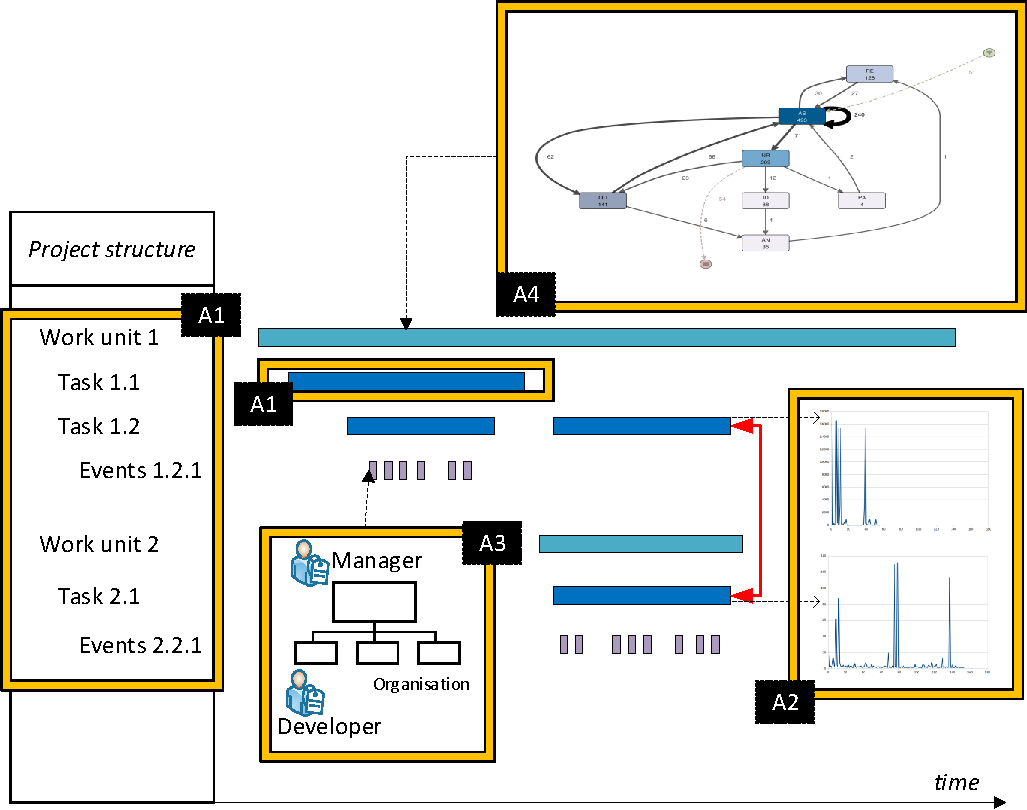
\includegraphics[width=\linewidth]{figures/big-solution2-crop.pdf}
	\caption{The empirical Gantt chart of software development. The four process perspectives combined.}
	\label{fig:big-solution}
\end{figure}

Research rigor and validity are ensured by evaluating the artifacts with the \gls{feds} \citep{Venable2016}. \Gls{feds} provides strategies for evaluating \gls{dsr} artifacts. More specifically, it takes into account two dimensions
\begin{inparaenum}[\itshape i)]
	\item the functional purpose of the
	evaluation (formative or summative); and 
	\item the paradigm of the evaluation (artificial or naturalistic).
\end{inparaenum} 
Moreover, it provides four steps for chinfinicaoosing an appropriate evaluation strategy
\begin{inparaenum}[\itshape i)]
	\item explicate the goals of the evaluation;
	\item choose the evaluation strategy or strategies
	\item determine the properties to evaluate; and
	\item design the individual evaluation episode(s). 
\end{inparaenum} In the following, we describe each designed artifact and their evaluation. 

\cite{Gregor2020} define a schema for defining \emph{design principles} so that they are understandable and useful in real world context. \todo{Shoud I define design principles according to their schema? This may be a good idea!}




%% Please add the following required packages to your document preamble:
% \usepackage{booktabs}
% \usepackage[normalem]{ulem}
% \useunder{\uline}{\ul}{}
% \usepackage{longtable}
% Note: It may be necessary to compile the document several times to get a multi-page table to line up properly
\begin{longtable}[c]{@{}p{1.2cm}p{2.5cm}p{5cm}p{3cm}p{4cm}@{}}
\toprule
\textbf{Artifact} & \textbf{Features}                              & \textbf{Goals}                                                                                                                                                                                                                                                           & \textbf{Evaluation}                                                                                                                                  & \textbf{Iteration episodes}                                                                                                   \\* \midrule
\endhead
%
\bottomrule
\endfoot
%
\endlastfoot
%
\textbf{A1}       & time information                               & General goal: has to be applicable, usable, simple and provide overview as well as detailed view                                                                                                                                                                         & Quick and simple: the technique is directly evaluated with real data                                                                                 & First iteration (formative): initial design of gantt chart                                                                    \\
                  & duration of activities                         & Rigor: assured by the design science approach                                                                                                                                                                                                                            &                                                                                                                                                      & Second iteration: evaluation of successful identification of events and project structure                                     \\
                  & structure of the project                       & Uncertainty and risk reduction: artifacts is technically infeasible, data is unavailable                                                                                                                                                                                 &                                                                                                                                                      & Third iteration: run of the tool on real projects and provide a visualization                                                 \\
                  & granularity of events                          & Ethics: “big-brother is watching you” effect on people                                                                                                                                                                                                                   &                                                                                                                                                      &                                                                                                                               \\
                  &                                                & Efficiency: find all time patterns, algorithm runs in a reasonably short time                                                                                                                                                                                            &                                                                                                                                                      &                                                                                                                               \\* \midrule
\textbf{A2}       & difference between different instances of work & General goal: has to be applicable, usable, simple and provide overview as well as detailed view                                                                                                                                                                         & Quick and simple: the technique is firstly evaluated with a toy example, then revised and applied to a large number of software development projects & First iteration (formative): initial design of artifact and results  visualizations                                           \\
                  & amount of changes                              & Rigor: assured by the iterations                                                                                                                                                                                                                                         &                                                                                                                                                      & Second iteration: revision and choice of final visualization                                                                  \\
                  & handle unstructured data from comments         & Uncertainty and risk reduction: artifacts is technically infeasible adressed by developing by smaller iterations, data is unavailable addresses by local copy, results interpretation is hard addressed by mining processes from text                                    &                                                                                                                                                      & Third iteration: evaluation of efficacy on retrieving features                                                                \\
                  & evolutionary analysis of changes               & Ethics: n/a because data is public                                                                                                                                                                                                                                       &                                                                                                                                                      & Fourth iteration: run the technique on toy exampe (artificial evaluation). Validate efficacy and usefulness. Revise artifact. \\
                  & uncover work dependencies                      & Efficiency: find all work dependencies in a reasonable time                                                                                                                                                                                                              &                                                                                                                                                      & Firfth iteration: run the technique on real data sets from GitHub projects (naturalistic evaluation)                          \\* \midrule
\textbf{A3}       & determine roles of users                       & General goal: has to aplicable and provide correct classification of roles                                                                                                                                                                                               & Quick and simple: the technique is evaluated with real data from industry partners                                                                   & First iteration (formative): initial design of simple artifact voted to a simple and structured represenation of the data     \\
                  & handle user comments                           & Rigor: assured by the iterations                                                                                                                                                                                                                                         &                                                                                                                                                      & Second iteration: selection of features and classifiers traininig. Selection of the best features and classifiers.            \\
                  & automatically classify resources               & Uncertainty and risk reduction: risk is that artifact incorrectly classifies reources, this is reduced by using different training sets from industry partners and otaining feedback                                                                                     &                                                                                                                                                      & Third iteration: evaluation of results with real data from partners and feeback                                               \\
                  &                                                & Ethics: there is a risk of obtaining information about people’s work. This is mitigated by NDA signed by the parties involved                                                                                                                                            &                                                                                                                                                      &                                                                                                                               \\
                  &                                                & Efficiency: evaluated in terms of precision and recall                                                                                                                                                                                                                   &                                                                                                                                                      &                                                                                                                               \\* \midrule
\textbf{A4}       & handle comments from forum conversations       & General goal: has to aplicable to pull requests and provide informative and reliable process models about the generation of an idea                                                                                                                                      & Technical risk and efficacy: the technique is firstly evaluated with an initial dataset, then revised and evaluated with other projects              & First iteration (formative): initial exploratory analysis on the applicability of process mining techniques on pull requests  \\
                  & discover a process model                       & Rigor: assured by the iterations                                                                                                                                                                                                                                         &                                                                                                                                                      & Second iteration: evaluation of process mining methods and assessment of statistical significance of results                  \\
                  &                                                & Uncertainty and risk reduction: risks are: 1) activities of business processes are not mapped correctly – mitigated by manual annotation 2) the resulting model is not informative – mitigated by statistical techniques voted to cluster traces into significant groups &                                                                                                                                                      & Third iteration: mine process models that are statistically significant and analyze the idea generation patterns              \\
                  &                                                & Ethics: n/a. Only data from open source repositories will be used                                                                                                                                                                                                        &                                                                                                                                                      &                                                                                                                               \\
                  &                                                & Efficiency: the artifact can deal with complex projects quickly                                                                                                                                                                                                          &                                                                                                                                                      &                                                                                                                               \\* \bottomrule
\end{longtable}

\subsection{Discovering the Temporal Perspective of the Software Development Process (Artifact A1)} 
%~\\\noindent\rule[1ex]{2.5cm}{2pt}~\\	
Design objectives of \textbf{A1} aure \begin{iiilist}
	\item has to be applicable, 
	\item usable, 
	\item simple and,
	\item provide overview as well as detailed view.
\end{iiilist} 
The following features are included: 
\begin{iiilist}
	\item time information,
	\item duration of activities,
	\item structure of the project, and
	\item roll-up and drill-down on granularity of events.
\end{iiilist}
Evaluation goals are 
\begin{iiilist}
	\item rigor,
	\item uncertainty and risk reduction,
	\item ethics, and
	\item efficiency.
\end{iiilist}
They are respectively addressed as follows. Rigor is assured by the design science approach. Uncertainty involves technical infeasibility and unavailuability of the data. Infeasibility risk is reduced by starting from the design of small artifacts with basic features and incrementally improve. Unavailability risk is reduced by replication of the dataset locally. An ethics problem may regard the “big-brother is watching you” effect on people. This will be solved considering only data from partners and public repositories. Efficiency is evaluated by measuring whether all time patterns are found in a reasonably short time.

This artifact is evaluated through a Quick \& Simple strategy \citep{Venable2016}, i.e., the technique is directly evaluated with real data. This will include three iteration episodes 
\begin{iiilist}
	\item initial design of Gantt chart (formative)
	\item evaluation of successful identification events, their duration and project structure; and 
	\item run of the tool on real projects and provide a visualization (summative).
\end{iiilist}



\subsection{Discovering the Case Perspective of the Software Development Process (Artifact A2)} 
%Addresses RQ2.
%~\\\noindent\rule[1ex]{2.5cm}{2pt}	
Design objectives of \textbf{A2} include applicability, simplicity and providing comparison of different cases. The following features are designed: 
\begin{iiilist}
	\item difference between work instances;
	\item measure of work: amount of changes;
	\item handle unstructured data from comments;
	\item evolutionary analysis of files; and
	\item uncover work dependencies.
\end{iiilist}
Evaluation goals are as follows. Rigor is assured by the iterations. Uncertainty and risk reduction consist in: technical infeasibility -- addressed through development by smaller iterations, data unavailability -- addressed by local replication of data, and simplicity of results -- addressed by exploiting user comments and derive informative process labels. Ethics problems do not arise as the data for this artifact is already public on GitHub. Efficiency is evaluated by finding all work dependencies in a reasonable time. 

This artifact is evaluated through a Technical risk \& Efficacy strategy (see \cite{Venable2016}), i.e., the technique is firstly evaluated with a toy example, then revised and applied to a large number of software development projects. Five iteration episodes are included: 
\begin{iiilist}
	\item initial design of artifact and results  visualizations(formative);
	\item revision and choice of final visualization;
	\item evaluation of efficacy on retrieving features;
	\item run the technique on toy example (artificial evaluation), validate efficacy and usefulness, revise artifact; and
	\item run the technique on real data sets from GitHub projects (summative and naturalistic evaluation).
\end{iiilist}



\subsection{Discovering the Organizational Perspective of the Software Development Process (Artifact A3)}
%~\\\noindent\rule[1ex]{2.5cm}{2pt}
Design objectives of \textbf{A3} include applicability and correct classification of roles. The following features are designed 
\begin{iiilist}
	\item determine roles of users;
	\item handle user comments; and
	\item automatically classify resources.
\end{iiilist}
Evaluation goals are as follows. Rigor is assured by the iterations. Uncertainty and risk reduction regard classification. Incorrect resource classification risk is reduced by using different training set data from industry partners and obtaining feedback. An ethics risk is about obtaining information about people's work. This is mitigated by NDAs signed by the parties involved. Efficiency is evaluated in terms of precision and recall. 

This artifact is evaluated through a Quick \& Simple strategy (\cite{Venable2016}), i.e., the technique is evaluated with real data from industry partners. Three iteration episodes are included: 
\begin{iiilist}
	\item initial design of the artifact voted to a simple and structured representation of the data (formative)
	\item exploration and selection of the best features and classifiers.
	\item evaluation of results with real data from partners and feedback (summative + naturalistic).
\end{iiilist}

\subsection{Discovering the Control-Flow Perspective of the Software Development Process (Artifact A4)} 
%Addresses RQ2.
%\rule{3cm}{1pt}
%~\\\noindent\rule[1ex]{2.5cm}{2pt}
Design objectives of \textbf{A4} are its applicability to pull requests and its functionality to provide informative and reliable process models about specific work patterns. The following features are designed.
\begin{iiilist}
	\item handle comments from forum conversations, and
	\item discover a process model.
\end{iiilist}
Evaluation goals are considered as follows. Rigor is assured by the iterations. Uncertainty and risk reduction the following
\begin{iiilist}
	\item activities of business processes are not mapped correctly -- mitigated by manual annotation; and
	\item the resulting model is not informative -- mitigated by statistical techniques voted to cluster traces into significant groups.
\end{iiilist} Ethics problems do not arise because only data from open source repositories will be used. Efficiency is measured by the extent to which the artifact can deal with complex projects quickly.

This artifact is evaluated through a Technical risk \& Efficacy strategy (see \cite{Venable2016}), i.e., the technique is firstly evaluated with an initial well-known dataset, then revised and evaluated with other projects. Three iteration episodes are included: 
\begin{iiilist}
	\item initial exploratory analysis on the applicability of \gls{pm} techniques on pull requests (formative);
	\item evaluation of \gls{pm} methods and assessment of statistical significance of results; and
	\item mine process models that are statistically significant and analyze the idea generation patterns (summative + naturalistic).
\end{iiilist}
%\end{description}



%Many scenarios in SHAPE require for automated solutions to respond to compliance problems. Compliance is regulated by rules and guidelines as for instance the European standards EN50126, EN50128, EN50129. These standards specify procedures and technical requirements for the development of programmable electronic systems that are used in railway control and protection applications. Thus, there is a clear need for transparency in the work that is done to make sure that it complies to the standards procedures. To this end, engineering projects are systematically verified by auditors who check if everything is done according to the rules imposed by the standards. This is typically done a posteriori and the challenge here is to able to understand all the process steps and their quality by looking at existing documentation. 
%It intends to support project managers or auditors who must validate the compliance of the work against existing rules and regulations. This involves building new artifacts in order to both partially automate compliance checking and help by providing better overviews on the existing process. 

%\begin{figure}
%	\centering
%	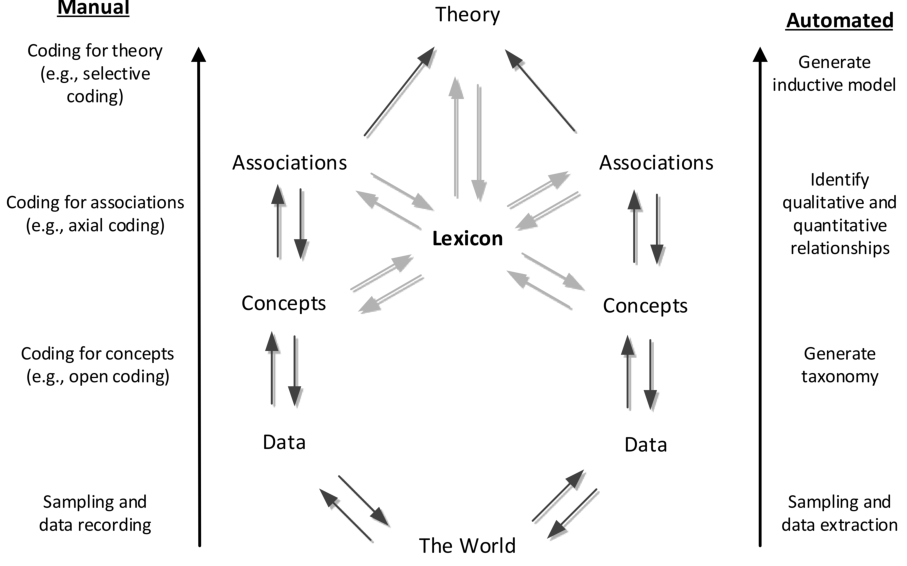
\includegraphics[width=0.7\linewidth]{figures/empirically-driven-theory-generation-1}
%	\caption{Empirically driven theory generation \citep{Berente2018}}
%	\label{fig:empirically-driven-theory-generation}
%\end{figure}


%\begin{description}
%	\item[Guideline 1 -- Design as an Artifact.] Design-science research must produce a viable artifact in the form of a construct, a model, a method, or an instantiation In my research, I use state-of-the-art techniques and develop new artifacts that allow to capture information from both structured and unstructured types of data. 
%	
%	\item[Guideline 2 -- Problem Relevance.] The objective of design-science research is to develop technology based solutions to important and relevant business problems. My research takes inspiration from real world needs which include human-centric safety-critical automated solutions in the railway domain.  
%	
%	\item[Guideline 3 -- Design Evaluation.] The utility, quality, and efficacy of a design artifact must be rigorously demonstrated via well-executed evaluation methods. The real world scenarios that I encounter in the SHAPE project require for novel solutions, which involve the design of new algorithms. Algorithms are converted to operational software. This operational software is an instantiated artifact \citep{Gregor2013}, which is then tested against real data. 
%	
%	\item[Guideline 4 -- Research Contributions.] Effective design-science research must provide clear and verifiable contributions in the areas of the design artifact, design foundations, and/or design methodologies. The contribution of my research can be positioned as a set of \emph{exapted} methods (cf. \gls{dsr} knowledge contribution framework \citep{Gregor2013}) from the fields of process mining and text mining, which contribute to a better understanding of projects. 
%	
%	\item[Guideline 5 -- Research Rigor.] Design-science research relies upon the application of rigorous methods in both the construction and evaluation of the design artifact. My research builds upon existing work from natural language processing \citep{de2006generating,Corro2013,klein2003accurate}, a number of \gls{vcs} mining works \citep{Banitaan2015,Allamanis2013,Vasilescu2015,Karimi2016,German2015}, and process mining.
%%	\cite[]{van2011process,rubin2007process,Rubin2014a,rubin2014agile}. 
%I plan to adopt mature methods from the mentioned works and construct my artifacts upon existing ones. 
%	
%	\item[Guideline 6 -- Design as a Search Process.] 
%	The search for an effective artifact requires utilizing available means to reach desired ends while satisfying laws in the problem environment. I plan to build my artifacts based on state-of-the-art methods and technology and follow both a rigorous process as the one described in \citep{Peffers2008} (cf. \cref{fig:DS-process}). Given the nature of my data, an exploratory phase may be required in the initial activity of this process. This may involve exploratory data analysis, as described in the data science process \citep[p.~41]{Schutt2013}
%	
%	\item[Guideline 7 -- Communication of Research.] Design-science research must be presented effectively both to technology-oriented as well as management-oriented audiences. I will use guidelines \citep{Gregor2013,Recker2015} in order to properly position my work. The main target will be \gls{bpm} conferences and journals. 
%	
%\end{description}


\section{Generated Datasets}
\label{sec:data-collection}

%\todo[inline]{Is this the best place for this section?}

This thesis includes the collection of and generation of datasets from real life software projects. These project data were collected both from industrial partners and from \gls{oss}. \Cref{tab:dataset} summarizes the available data. Logs from industrial partner are concerned with specific development activities (e.g., building railway interlocking-system software) and include a sufficient number of events that cover one software release. Logs from \gls{oss} were manually extracted by GitHub repositories. A tool has then been devised to parse these data and use them to populate a database. An original dataset is represented by Github pull requests. This dataset contains a list of manually annotated pull requests using the coding scheme by \cite[]{Majchrzak2016}. An additional output of this thesis will be the creation of a larger dataset using a machine learning approach that is able to automatically categorize pull requests in the classes given by \cite[]{Majchrzak2016}.

% Please add the following required packages to your document preamble:
% \usepackage{booktabs}
\begin{table}[]
\centering
\caption{Available datasets for this thesis}
\label{tab:dataset}
\begin{tabular}{@{}m{2.5cm}m{9cm}@{}}
\toprule
\textbf{Event Logs} & \textbf{Description} \\ \midrule
SHAPE & Industry \gls{vcs} from software development in the railway domain \\
Github & Logs from real world \gls{oss} development \\
Github pull requests & Manually annotated pull requests from one real life open source project \\
Jira & Log data from \gls{its} from industry partner \\
Asana & Generated dataset from project management tool of industrial partner \\
Kibana & Event traces from distributed process-agnostic enviroment used to handle communication among several processes \\ \bottomrule
\end{tabular}
\end{table}

%\subsection{Expected Outcome}
%
%In addition to an original dataset, this doctoral thesis is expected to produce outcomes that help the project manager analyze his software development processes. To this end new approaches in the form of artifacts \citep{Peffers2008} will be devised. These artifacts will serve as proofs-of-concept for the applicability of the research. In particular, the artifacts must address each of the four process aspects. Therefore, the outcome is categorized according to the research questions derived in \Cref{sec:problem-definition} as follows.
%
%\begin{itemize}	
%	\item \textbf{Artifact A1: Mining the Time Perspective (RQ1)}. Novel technique that allows for gaining transparency on the time perspective of software development work.	For instance, and artifact that explicits what are the durations of tasks and when are actual tasks executed.
%	
%	\item \textbf{Artifact A2: Mining the Case Perspective (RQ2)}. Novel technique that allows for gaining transparency on the case perspective of software development work. For instance, an artifact that explicits how the different cases are handled and whether there is any dependency of work that might influence the case execution. 
%	
%	\item \textbf{Artifact A3: Mining the Organizational Perspective (RQ3)}. Novel technique that allows for gaining transparency on the organizations aspect of software development work. For instance, an artifact that explicits which are the actual roles software developers are covering and which is the organizational network. 
%	
%	\item \textbf{Artifact A4: Mining the Control-Flow Perspective (RQ4)}. Novel technique that allows for gaining transparency on the control-flow perspective of software development work. For instance, an artifact that allows for abstracting from data which is order of activities that are executed to accomplish a certain task or goal in software development.	
%\end{itemize}

%\Cref{fig:big-solution} shows the overall information coming from combining the four perspectives into a Gantt chart that is more informative to managers. 




\section{Research Contributions}
\label{sec:intro-contributions}

%\todo[inline]{Summarize contributions beyond the papers. E.g., visualisation, conceptualisation of process-oriented business processes, etc. Elaborate more and think of further contributions.}

This doctoral thesis aims at bridging the gap between automatic analysis of software development data and process mining. It provides analyses techniques that help learning specific characteristics of the software process from its trace data. Beyond the publications, this thesis makes the following contributions.

\begin{itemize}
	
	\item \textbf{Conceptualization of project-oriented business processes.} Processes have been seen so far as repeatable endeavors. However, there are processes which are not repeated exactly in the same way twice. This is the case with project-oriented business processes. Such processes, are conducted as projects, in that they are usually planned a priori and run under limited resources. 
	
	\item \textbf{Visualization.} Existing techniques in the software engineering area are able to provide several possible views on the software development. Major visualization techniques can be divided into graph-based \citep{DBLP:journals/ijseke/GermanH06,DBLP:journals/smr/GreevyDG06}, notation-based \citep{DBLP:conf/wcre/McNairGW07}, matrix-based \citep{DBLP:conf/icsm/GirbaDL04} and metaphor-based \citep{DBLP:conf/vissoft/WettelL07}. These visualization techniques help in multiple ways, such as understanding code smells, refactoring, evolution, distribution of work etc. However, most of the works in software engineering area are not process-aware. Thus, this thesis aims at researching the most suitable visualization techniques that help understanding the work process that lays behind software development. 	

	\item \textbf{Extension of the scope of process mining.} Process mining techniques rely on structured data. These data are typically captured by the standard XES \citep{xes-standard:2015} which defines precisely the input of process mining techniques. This work extends process mining towards mining processes also from data that are not directly represented in the XES standard. 
	
	\item \textbf{Datasets for further research.} During the course of this research a number of datasets have been generated. These datasets are available for further use by researchers who want to replicate these studies or pursue different goals using the same concepts that this thesis provides. 
	
\end{itemize}



\section{Thesis Structure}
\label{sec:intro-structure}

%\todo[inline]{Elaborate more the description of what the sections provide.}

This thesis is structured as follows. 

\begin{itemize}
	\item \textbf{Chapter 1: Introduction} motivates research on the topic of mining processes from software repositories. This chapter also scopes the problem addressed by this dissertation and provides an overall guide to the content of this manuscript.
	
	\item \textbf{Chapter 2: Research Background} presents the body of knowledge which inform this thesis. 
%	\item \textbf{Chapter 3: Data-Driven Approaches to Analyzing the Software Process} 
	This chapter also elaborates on existing solutions and techniques that are present in the literature which are used as a base to develop new artifacts for mining the software process. 
	
	\item \textbf{Chapter 3: Discovering the Temporal Perspective} tackles the problem of discovering the temporal aspect (RQ1) of the software development process. A visualization technique is presented that simplifies the managers' understanding of such perspective.
	
	\item \textbf{Chapter 4: Discovering the Case Perspective}  presents an approach that helps understanding how different artifacts co-evolve in software development. With this approach, it is possible to compare how similarly different artifacts evolve and consequently cluster them into similar development cases (RQ2).  
	
	\item \textbf{Chapter 5: Discovering the Organizational Perspective} tackles the problem of automatically identifying emerging roles in software development. Thus, a technique for classifying human-resources (RQ3) based on factual data is presented.
	
	\item \textbf{Chapter 6: Discovering the Control-Flow Perspective} complements the techniques presented in previous chapter with the information about which activities were executed by resources. These activity labels along with the temporal help understanding the control-flow (RQ4) of the development process.
	
	\item \textbf{Chapter 7: Further Discovery Approaches} presents two more approaches which use trace data to gather insights on the process. The first approach provides a showcase where trace data analyses of software repositories is combined with subjective information from questionnaire. Mixing these methods helps to better identify issues in and suggest interventions based on facts. The second approach leverages on speech act theory to better understand the work done in by software developers. Unstructured data from conversations is used to analyze collaboration and derive a process (RQ4).
	
	\item \textbf{Chapter 8: Conclusion} summarizes the main findings. Further more, it discusses their implications along with future research. 
	 	
\end{itemize}


\section{Publications}
\label{sec:intro-related-publications}

This dissertation has led to the publications listed below.\\

\noindent {Mining the Time Perspective(\textbf{RQ1}):}~\citep{DBLP:conf/bpm/BalaCMRP15}
\begin{itemize}
\item \textbf{Bala, S.}, Cabanillas, C., Mendling, J., Rogge-Solti, A., and Polleres, A.: \textit{Mining Project-Oriented Business Processes}. In Hamid Reza Motahari-Nezhad, Jan Recker, and Matthias Weidlich, editors, BPM 2015, Innsbruck, Austria, volume 9253 of Lecture Notes in Computer Science, pages 425--440. Springer, 2015. 
\end{itemize}	
\noindent {Mining the Case Perspective (\textbf{RQ2}):}~\citep{DBLP:conf/bpm/BalaRGBMS17}.
\begin{itemize}
	\item \textbf{Bala, S.}, Revoredo, K., de A.R. Gonçalves, J.C., Baião, F., Mendling, J., Santoro, F.: \textit{Uncovering the Hidden Co-evolution in the Work History of Software Projects}. In: Carmona, J., Engels, G., and Kumar, A. (eds.) Business Process Management - 15th International Conference, BPM 2017, Barcelona, Spain, September 10-15, 2017, Proceedings. pp. 164--180. Springer (2017). 
\end{itemize}
\noindent {Mining the Organizational Perspective (\textbf{RQ3}):} \citep{DBLP:conf/edoc/AgrawalATBRT16}.
\begin{itemize}
	\item Agrawal, K., Aschauer, M., Thonhofer, T., \textbf{Bala, S.}, Rogge-Solti, A., Tomsich, N.: \textit{Resource Classification from Version Control System Logs}. In: Proceedings - IEEE International Enterprise Distributed Object Computing Workshop, EDOC Workshop. pp. 249--258 (2016). 
\end{itemize}
\noindent {Mining the Control-Flow Perspective (\textbf{RQ4}):} \citep{DBLP:conf/ifip8-1/BalaKM20}
\begin{itemize}
	\item \textbf{Bala, S.}, Kneringer, P., \& Mendling, J.: \textit{Discovering Activities in Software Development Processes}. In: CEUR Workshop Proceedings. (2020)
\end{itemize}

\noindent The following publications are related to the requirements.
\begin{itemize}
	
\item \textbf{Bala, S.}, Cabanillas, C., Haselböck, A., Havur, G., Mendling, J., Polleres, A., Sperl, S., Steyskal, S.: \textit{A Framework for Safety-Critical Process Management in Engineering Projects}. In: Ceravolo, P. and Rinderle-Ma, S. (eds.) Data-Driven Process Discovery and Analysis- SIMPDA. pp. 1--27. Springer (2015). \cite[]{Bala2017} -- Related to \textbf{RQ1} \& \textbf{RQ3}.
	
\item \textbf{Bala, S.}, Havur, G., Sperl, S., Steyskal, S., Haselböck, A., Mendling, J., Polleres, A.: \textit{SHAPEworks: A BPMS extension for complex process management}. In: CEUR Workshop Proceedings. pp. 50--55 (2016). \cite[]{Bala2016} -- Related to \textbf{RQ1} \& \textbf{RQ3}.
	
\end{itemize}

\noindent Early stage concepts of this research (research proposal) have been presented in doctoral consortium and conference.
\begin{itemize}
	\item \textbf{Bala, S.}: \textit{Mining projects from structured and unstructured data}. In: CEUR Workshop Proceedings (2017). \cite[]{Bala2017b}

	\item \textbf{Bala, S.}, Mendling, J.: \textit{Monitoring the Software Development Process
		with Process Mining}. In Boris Shishkov, editor, Business Modeling and Software
	Design, volume 319 of Lecture Notes in Business Information Processing, 2018 \citep{Bala2018b} 	
\end{itemize}	
	

\noindent Further work published in the \gls{bpm} area is the following.

\begin{itemize}
	\item Woli\'nski, B., \textbf{Bala, S.}: \textit{Comprehensive Business Process Management at Siemens: Implementing Business Process Excellence}. In: vom Brocke, J. and Mendling, J. (eds.) Business Process Management Cases: Digital Innovation and Business Transformation in Practice. pp. 111--124. Springer International Publishing, Cham (2018). \cite[]{Wolinski2018}
	
	\item \textbf{Bala, S.}, Mendling, J., Schimak, M. and Queteschiner, P., 2018, October. \textit{Case and activity identification for mining process models from middleware}. In IFIP Working Conference on The Practice of Enterprise Modeling (pp. 86-102). Springer, Cham. \citep{DBLP:conf/ifip8-1/BalaMSQ18}
	
	\item Azemi, E., \textbf{Bala, S.}: \textit{Exploring BPM adoption and strategic alignment of processes at Raiffeisen Bank Kosovo}. In: BPM (Industry Forum). pp. 37–48. CEUR-WS.org (2019). \cite[]{DBLP:conf/bpm/AzemiB19}
	
	\item Vidgof, M., Djurica, D., \textbf{Bala, S.}, and Mendling, J. (2020). \textit{Cherry-picking from
	spaghetti: Multi-range filtering of event logs}. In BPMDS/EMMSAD@CAiSE,
	volume 387 of Lecture Notes in Business Information Processing, pages 135–149.
	Springer. \citep{DBLP:conf/caise/VidgofDBM20}
	
	\item Vidgof, M., Djurica, D., \textbf{Bala, S.}, Mendling, J.: \textit{Interactive Log-Delta-Analysis using Multi-Range Filtering}. Software and Systems Modeling. (to appear), (2021). \citep{Vidgof2021}
	
	\item Azemi, E., \textbf{Bala, S.}: \textit{Exploring BPM adoption and strategic alignment of processes at Raiffeisen Bank Kosovo}. In: vom Brocke, J., Mendling, J., Rosemann, M. (eds.) Business Process Management Cases. Springer (2021). \citep{Azemi2021}
	
	\item Waibel, P., Novak, C., \textbf{Bala, S.}, Revoredo, K., Mendling, J.: \textit{Analysis of Business Process Batching Using Causal Event Models}. In: Leemans, S.J.J. and Leopold, H. (eds.) ICPM Workshops. pp. 1–13. Springer Nature Switzerland AG (2021). \citep{Waibel2021}
	
\end{itemize}

%\noindent From ongoing work the following publications are expected.
%\begin{itemize}
%	\item Case study on tool productivity. Collaboration with researchers from the University of Ljubljana to be submitted to an A-ranked journal on information systems. -- Related to \textbf{RQ1}, \textbf{RQ3} and \textbf{RQ4}.
%	
%	\item Process mining pull requests for identifying idea-creation patterns. Collaboration with researchers from Stevens Institute of Technology to be submitted to a class A journal on information systems -- Related to \textbf{RQ4}.
%	
%	\item Wurm, B., \textbf{Bala, S.}, Kremser, W., Mendling, J., Minaar, R., Strauss, E.: Working title: \textit{How holacratic organizations use information technology to prevent inertia of organizational rule networks}.  to submitted to Information Systems Research 
%		
%\end{itemize}



\chapter{Research Background}
\label{ch2:problem-background}

\section{Software Process}
\label{sec:ch2-software-process}

What is the software process. Humphrey: (rationally) Managing the software process?

\section{Theorizing the Software Process}
\label{sec:ch2-theorizing}

\subsection{Organization Routines}
\label{subsec:org-stud}

\subsection{Coordination Theory}

\subsection{Business Process Management}

\subsection{Language-Action (Perspective)}

Winograd \& Flores~\citep{Winograd1986a}

\section{Tool Support for Software Development Processes}
\label{sec:ch2-tool-support}

Talk about what tools are used.
Especially what tools/repositories I analyze. 



\section{Software Process Monitoring }
\label{sec:ch2-sw-p-monitoring}

\subsection{What is important to be monitored}

\subsection{How far it is difficult}

\section{Research Questions}
\label{sec:ch2-research-questions}

Summarize the gap here. Make it clear that the bigger research question is divided into 4 research questions. It is split on perspective. 
Refer to the main RQ as research problem (RP). Then you have RQ1, RQ2, ... .


Before formulating the research questions, build the context with the terminology. Kate says "RQ1. Which activities and when?".

\todo[inline]{Terminology must be defined somewhere. Maybe we need a preliminaries section. For example, what is an artifact? Define it.}

Addressed in the main chapters.

Type of work: testing, development, documentation, bug-fixing, feature specification. 

Assumption is that the project is structured in folders. A project is broken down into parts. Parts can be mapped to folders.

RQ: How can we make use of project event data to gather insights about the software development process that are
informative to managers

\begin{description}
	\item[RQ1] What type of work was performed? 
	(Paul's thesis addresses this.)
	\item[RQ2] How were activities performed in the different parts of the project?
	\item[RQ3] description
\end{description}



%\chapter{Analysis Techniques for Software Processes}
%\label{chap:ch3-solution-background}
%
%\todo[inline]{This is still related work, but here we talk about the "solutions". Check for overlap with Research Background and the other chapters below.}
%\todo[inline]{Elaborate on Section 3.2, 3.3}


%This chapter is concerned with data-driven approaches used in literature to \emph{solutions}, which help tackling the problem of monitoring software development. Four disciplines provide the necessary theoretical and practical knowledge upon which this thesis is built. Thus, this chapter presents these four disciplines as follows. \Cref{sec:process-mining} briefly describes the area of process mining. \Cref{sec:msr} describes contributions from the area of mining software repositories. \Cref{sec:visualization} provides an overview on the area of software visualization. \Cref{sec:text-mining} shortly describes the area of text mining, used for extracting knowledge from unstructured data. Finally, \Cref{sec:summary-of-relevant-techniques} summarizes these solutions. 



%\section{Text Mining}
%\label{sec:text-mining}
%
%%\subsection{Description of the field} 
%
%\Gls{tm} refers to the process of deriving information from natural language text. It relates to data mining in the aspect that both strive to extract meaningful information from raw data. However, data mining is characterized as the extraction of implicit, previously unknown, and potentially useful information from data, whereas with text mining the information to be extracted is clearly and explicitly stated in the text~\citep{Witten2004}. 
%\Gls{tm} can be regarded as going beyond information access to further help users analyze and digest information and facilitate decision making. There are also many applications of text mining where the primary goal is to analyze and discover any interesting patterns, including trends and outliers in text data.
%Although text mining is mostly about \gls{nlp}~\citep{jurafsky2014speech}, it embraces also applications that go beyond. For example, it analyzes linkage structures such as the citations in the academic literature and hyperlinks in the Web literature, both useful sources of information that lie outside the traditional domain of \gls{nlp}. 

%The main types of text mining are the following.
%
%%\Cref{tab:text-mining-overview} gives a compact overview on the types of text mining and some example references.
%%
%%\begin{table}[!h]
\centering
\caption{Overview on text mining types}
\label{tab:text-mining-overview}
\vspace{5pt}
%\resizebox{\textwidth}{!}{
\begin{tabular}{m{4cm}m{5cm}m{4cm}}
\toprule
\textbf{Type}                         & \textbf{Task}                                                                                                                   & \textbf{References}                                                                                           \\ \midrule
Information extraction       & Filling in templates from natural language text                                                                        & \cite{cowie1996information}, \cite{mooney1999relational}, \cite{seymore1999learning}, \cite{banko2007open} \\ %\midrule
Topic detection and tracking & Finding and following new events in a stream                                                                           & \cite{Allan1998}, \cite{wayne2000multilingual}                                                  \\ %\midrule
Summarization                & Reducing the content obtained from text documents, still keeping the topic                                             & \cite{aggarwal2012mining}, \cite{gupta2009survey}                                                    \\ %\midrule
Categorization               & Identifying the main themes of a document                                                                              & \cite{sebastiani2002machine}, \cite{joachims1998text}                                                \\ %\midrule
Clustering                   & Group similar documents by predefined topics                                                                           & \cite{zhao2001criterion}, \cite{fung2003hierarchical}, \cite{aggarwal2012mining}                     \\ %\midrule
Concept Linkage              & Connect related documents by identifying their shared concepts                                                         & \cite{maedche2000mining}, \cite{fan2006tapping}, \cite{gupta2009survey}                             \\ %\midrule
Information visualization    & Visualizing large textual sources                                                                                      & \cite{wong1999visualizing}, \cite{Mostafa2013}                                                       \\ %\midrule
Question answering           & Automatically answer questions posed by humans                                                                         & \cite{katz1997sentence}, \cite{kwok2001scaling}, \cite{aggarwal2012mining}                           \\ %\midrule
Association rule mining      & Study the relationships and implications among topics or descriptive concepts that are used to characterize a corpus & \cite{agrawal1993mining}, \cite{agrawal1994fast}, \cite{hu2010}                                      \\ \bottomrule
\end{tabular}
%}
\end{table}
%
%\begin{description}
%	\item[Information extraction.] 
%%	Information extraction is used to refer to the task of filling in templates from natural language text. The goal is to extract from the documents (which may be in a variety of languages) salient facts about prespecified types of events, entities or relationships. These facts are then usually entered automatically into a database, which may then be used to analyze the data for trends, to give a natural language summary, or simply to serve for on-line access. Traditional information extraction techniques~\citep{cowie1996information,mooney1999relational} leverage on rule-based systems that match predefined linguistic patterns. More recently, work on named entity recognition uses statistical machine learning methods~\citep{seymore1999learning}. A tool that uses unsupervised learning can be found in \citep{banko2007open}.
%	It is the task of filling in templates from natural language text. The goal is to extract from the documents (which may be in a variety of languages) salient facts about prespecified types of events, entities or relationships. They can be used to analyze the data for trends, to give a natural language summary, or simply to serve for on-line access. Typical examples can be found in~\citep{cowie1996information,mooney1999relational,seymore1999learning,banko2007open}.
%	
%	\item[Topic detection and tracking.] 
%%	\Gls{tdt} was a DARPA-sponsored initiative to investigate on finding and following new events in a stream of broadcast news stories. The \gls{tdt} problem consists of three major tasks: (1) \emph{segmenting} a stream of data, especially recognized speech, into distinct stories; (2) \emph{identifying} those news stories that are the first to discuss a new event occurring in the news; and (3) given a small number of sample news stories about an event, \emph{finding} all \emph{following} stories in the stream.
%%	The work of \citep{allan2002introduction} has formally defined this problem and proposed the initial set of algorithms for the task. Main subtasks of TDT, as identified in \citep{wayne2000multilingual} are 
%%	(i) finding topically homogeneous regions (segmentation); (ii) finding additional stories about a given topic (tracking); (iii) detecting and threading together new topics (detection); (iv) Detecting new topics (first story detection); and (v) Deciding whether stories are on the same topic (linking). An example of a real-world TDT system is Google Alerts\footnote{\url{https://www.google.com/alerts}}.
%	The \gls{tdt} problem consists of three major tasks: (1) \emph{segmenting} a stream of data, especially recognized speech, into distinct stories; (2) \emph{identifying} those news stories that are the first to discuss a new event occurring in the news; and (3) given a small number of sample news stories about an event, \emph{finding} all \emph{following} stories in the stream.
%	Typical examples can be found in~\citep{wayne2000multilingual,allan2002introduction}.
%	%	The work of \citep{allan2002introduction} has formally defined this problem and proposed the initial set of algorithms for the task. Main subtasks of TDT, as identified in \citep{wayne2000multilingual} are 
%	%	(i) finding topically homogeneous regions (segmentation); (ii) finding additional stories about a given topic (tracking); (iii) detecting and threading together new topics (detection); (iv) Detecting new topics (first story detection); and (v) Deciding whether stories are on the same topic (linking). An example of a real-world TDT system is Google Alerts\footnote{\url{https://www.google.com/alerts}}.
%	
%	\item[Summarization.] 
%%	Summarization is the task of reducing the content obtained from text documents, still keeping a brief overview on a topic that they treat. Summarization techniques generally fall into two categories \citep{Aggarwal2015}. In extractive summarization, a summary consists of information units extracted from the original text; in contrast, in abstractive summarization, a summary may contain {\textquotedblleft synthesized\textquotedblright} information units that may not necessarily occur in the text document. An automatic summarization process can be divided into three steps \citep{gupta2009survey}: (1) the \emph{preprocessing} step where a structured representation of the original text is obtained; (2) the \emph{processing} step where an algorithm must transform the text structure into a summary structure; and (3) the \emph{generation} step where the final summary is obtained from the summary structure. 
%%	A plethora of text summarization tools can be found online. A few examples are the open source libraries such Open Text Summarizer\footnote{\url{https://www.splitbrain.org/services/ots}}, Sumplify\footnote{\url{http://sumplify.com/}} and Online summarize tool\footnote{\url{http://www.tools4noobs.com/summarize/}}.
%Summarization is the task of reducing the content obtained from text documents, still keeping a brief overview on a topic that they treat. Typical examples of can be found in~\citep{gupta2009survey,Aggarwal2015}. Some open source libraries are Open Text Summarizer\footnote{\url{https://www.splitbrain.org/services/ots}}, Sumplify\footnote{\url{http://sumplify.com/}} and Online summarize tool\footnote{\url{http://www.tools4noobs.com/summarize/}}.
%	
%	\item[Categorization.] 
%%	Categorization aims at identifying the main themes of a document. This translates into assigning natural language documents to predefined categories according to their content~\citep{sebastiani2002machine}. Categorization often relies on a thesaurus for which topics are predefined, and relationships are identified by looking for broad terms, narrower terms, synonyms, and related terms. \Glspl{svm} are used to automatically learn text classifiers from examples~\citep{joachims1998text}. Categorization tools usually rank documents according to how much of their content fits in a particular topic. 
%%	
%	Categorization aims at assigning natural language documents to predefined categories according to their content. 
%%	Categorization often relies on a thesaurus for which topics are predefined, and relationships are identified by looking for broad terms, narrower terms, synonyms, and related terms. 
%	\Glspl{svm} are used to automatically learn text classifiers from examples. Typical examples can be found in~\citep{joachims1998text,sebastiani2002machine}.
%%	Categorization tools usually rank documents according to how much of their content fits in a particular topic. 
%	
%	\item[Clustering.] 
%%	Clustering is a technique used to group similar documents, but it differs from categorization in that documents are clustered on the fly instead of through predefined topics. Documents can also appear in multiple subtopics, ensuring that useful documents are not omitted from the search results. A basic clustering algorithm creates a vector of topics for each document and measures the weights of how the document fits into each cluster. A survey of clustering algorithms can be found in \citep{Aggarwal2015}. 
%	Clustering is a technique used to group similar documents, but it differs from categorization in that documents are clustered on the fly instead of through predefined topics. 
%%	Documents can also appear in multiple subtopics, ensuring that useful documents are not omitted from the search results. A basic clustering algorithm creates a vector of topics for each document and measures the weights of how the document fits into each cluster. 
%A literature review of clustering algorithms can be found in \citep{Aggarwal2015}. 
%	
%	\item[Concept Linkage.] 
%%	Concept-linkage tools connect related documents by identifying their shared concepts, helping users find information they perhaps would not have found through traditional search methods~\citep{gupta2009survey}. It promotes browsing for information rather than searching for it. For example, a text mining software solution may easily identify a transitive closure in a set of topics \{X, Y, Z\}, i.e., a link between X and Y, a link between Y and Z, %. But the text mining tool could also detect a potential 	and a link between X and Z. %(i.e. transitive closure on the set of topics), something that a human researcher has not come across yet.	With large sets of data, such a relationship could be disregarded by humans. %because of the large volume of information s/he would have to sort through to make the connection.
%	Concept-linkage tools connect related documents by ide\section{Text Mining}
%\label{sec:text-mining}
%
%%\subsection{Description of the field} 
%
%\Gls{tm} refers to the process of deriving information from natural language text. It relates to data mining in the aspect that both strive to extract meaningful information from raw data. However, data mining is characterized as the extraction of implicit, previously unknown, and potentially useful information from data, whereas with text mining the information to be extracted is clearly and explicitly stated in the text~\citep{Witten2004}. 
%\Gls{tm} can be regarded as going beyond information access to further help users analyze and digest information and facilitate decision making. There are also many applications of text mining where the primary goal is to analyze and discover any interesting patterns, including trends and outliers in text data.
%Although text mining is mostly about \gls{nlp}~\citep{jurafsky2014speech}, it embraces also applications that go beyond. For example, it analyzes linkage structures such as the citations in the academic literature and hyperlinks in the Web literature, both useful sources of information that lie outside the traditional domain of \gls{nlp}. 
%ntifying their shared concepts, helping users find information they perhaps would not have found through traditional search methods. Typical examples can be found in~\citep{gupta2009survey}. 
%%	It promotes browsing for information rather than searching for it. For example, a text mining software solution may easily identify a transitive closure in a set of topics \{X, Y, Z\}, i.e., a link between X and Y, a link between Y and Z, %. But the text mining tool could also detect a potential 
%%	and a link between X and Z. %(i.e. transitive closure on the set of topics), something that a human researcher has not come across yet 
%%	With large sets of data, such a relationship could be disregarded by humans. %because of the large volume of information s/he would have to sort through to make the connection.
%	
%	\item[Information Visualization.] 
%%	Information visualization aims at visualizing large textual sources in such a way that the content can be displayed in a hierarchy or map and provides browsing feat\section{Text Mining}
%\label{sec:text-mining}
%
%%\subsection{Description of the field} 
%
%\Gls{tm} refers to the process of deriving information from natural language text. It relates to data mining in the aspect that both strive to extract meaningful information from raw data. However, data mining is characterized as the extraction of implicit, previously unknown, and potentially useful information from data, whereas with text mining the information to be extracted is clearly and explicitly stated in the text~\citep{Witten2004}. 
%\Gls{tm} can be regarded as going beyond information access to further help users analyze and digest information and facilitate decision making. There are also many applications of text mining where the primary goal is to analyze and discover any interesting patterns, including trends and outliers in text data.
%Although text mining is mostly about \gls{nlp}~\citep{jurafsky2014speech}, it embraces also applications that go beyond. For example, it analyzes linkage structures such as the citations in the academic literature and hyperlinks in the Web literature, both useful sources of information that lie outside the traditional domain of \gls{nlp}. 
%ures, in addition to simple search. For instance, governments or police can identify terrorist networks in a map and identify crimes that were previously unconnected~\citep{gupta2009survey}.
%	Information visualization aims at visualizing large textual sources in such a way that the content can be displayed in a hierarchy or map and provides browsing features, in addition to simple search. Typical examples can be found in~\citep{gupta2009survey}.
%	
%	\item[Question Answering.] 
%%	Another application area of developed text-mining technologies, along with the natural language processing, is natural language features Question Answering (QA). QA is concerned with building systems that automatically answer questions posed by humans in a natural language.
%%	One of the first Query Answering tools was START\footnote{\url{http://start.csail.mit.edu/index.php}}, developed in the work of \citep{katz1997sentence}. Question answering has been extensively used in Biomedical domain for aiding researchers and health care professionals in managing the continuous growth of information.	
%%	Another application area of developed text-mining technologies, along with the natural language processing, is natural language features Question Answering (QA). 
%	QA is concerned with building systems that automatically answer questions posed by humans in a natural language. One of the first Query Answering tools was START\footnote{\url{http://start.csail.mit.edu/index.php}}, developed in the work of \citep{katz1997sentence}. 
%%	Question answering has been extensively used in Biomedical domain for aiding researchers and health care professionals in managing the continuous growth of information.
%	
%	\item[Association Rule Mining.] 
%%	The focus of association rules mining is to study the relationships and implications among topics, or descriptive concepts, that are used to characterize a corpus. The work of \citep{agrawal1994fast} shows how it is possible to discover association rules from massive data from databases, referred to as \emph{basket} data. The same approach can be followed by constructing a database of rules using information extraction methods and subsequently applying techniques, e.g. \citep{hu2010}, to uncover hidden associations in the database. For instance, a rule might be that 98\% of customers that purchase tires and auto accessories also get automotive services done. This suggests that association rules can be captured as if/then patterns. Criteria such as support and confidence~\citep{agrawal1993mining} are used to identify the most important relationships. Support is an indication of how frequently the items appear in the database. Confidence indicates the number of times the if/then statements has been found to be true.
%	The focus of association rules mining is to study the relationships and implications among topics, or descriptive concepts, that are used to characterize a corpus. Typical examples can be found in~\citep{agrawal1993mining,agrawal1994fast,hu2010}.
%%	The work of \citep{agrawal1994fast} shows how it is possible to discover association rules from massive data from databases, referred to as \emph{basket} data. The same approach can be followed by constructing a database of rules using information extraction methods and subsequently applying techniques, e.g. \citep{hu2010}, to uncover hidden associations in the database. For instance, a rule might be that 98\% of customers that purchase tires and auto accessories also get automotive services done. This suggests that association rules can be captured as if/then patterns. Criteria such as support and confidence~\citep{agrawal1993mining} are used to identify the most important relationships. Support is an indication of how frequently the items appear in the database. Confidence indicates the number of times the if/then statements has been found to be true.
%	
%\end{description}

%\subsection{Contribution to the research questions} 
%
%%\todoinline{more details}
%
%%My research involves unstructured data in the form of word processor documents, emails, user forums, and commit messages from \gls{vcs}. Text mining algorithms can be combined to quantitative data to gather information about project work. For example, topics models can be combined to time-clustered messages from pull request comments. In this way it is possible order to discover ``hot topics" (e.g. deliverable, milestone, meeting, etc) during project development. More in general, text mining techniques help with preprocessing the data and retrieving relevant information. Successively, this information can be brought together to create a structured event log in the \gls{xes} format. Therefore, text mining research serves and a preprocessing technique to facilitate process extraction. Especially, it helps as follows. 
%
%\gls{nlp} based approaches have been used to identify process cases and activities. Contributions in this group the have focused on process discovery. \citep{Goncalves2009a} discovered a model from group stories. \citep{Friedrich2011} reaches 77\% of accuracy in reconstructing process models from text. \citep{DoNascimento2012} analyze legacy systems code to infer business process rules and activities. \citep{DiCiccio2013} use \gls{nlp} to aid the extraction of artful processes from knowledge workers emails.
%
%There are also works that help with information extraction. \citep{Maalej2010} use \gls{nlp} for automating descriptions of work sessions by analyzing developers' informal text notes about their tasks. Developers are then classified into two classes based on their behavior: developers who use problem information to refer to their current activity and developers who refer to task and requirements. \citep{Kouters2012} developed an identity merging algorithm based on Latent Semantic Analysis (LSA) to disambiguate user emails. \citep{Licorish2014} mined developer comments to understand their attitudes.
%
%Role discovery has also seen contributions. A number of algorithms have b\subsection{Contribution to the research questions} 

%\todoinline{more details}

%My research involves unstructured data in the form of word processor documents, emails, user forums, and commit messages from \gls{vcs}. Text mining algorithms can be combined to quantitative data to gather information about project work. For example, topics models can be combined to time-clustered messages from pull request comments. In this way it is possible order to discover ``hot topics" (e.g. deliverable, milestone, meeting, etc) during project development. More in general, text mining techniques help with preprocessing the data and retrieving relevant information. Successively, this information can be brought together to create a structured event log in the \gls{xes} format. Therefore, text mining research serves and a preprocessing technique to facilitate process extraction. Especially, it helps as follows. 

%\gls{nlp} based approaches have been used to identify process cases and activities. Contributions in this group the have focused on process discovery. \citep{Goncalves2009a} discovered a model from group stories. \citep{Friedrich2011} reaches 77\% of accuracy in reconstructing process models from text. \citep{DoNascimento2012} analyze legacy systems code to infer business process rules and activities. \citep{DiCiccio2013} use \gls{nlp} to aid the extraction of artful processes from knowledge workers emails.
%
%There are also works that help with information extraction. \citep{Maalej2010} use \gls{nlp} for automating descriptions of work sessions by analyzing developers' informal text notes about their tasks. Developers are then classified into two classes based on their behavior: developers who use problem information to refer to their current activity and developers who refer to task and requirements. \citep{Kouters2012} developed an identity merging algorithm based on Latent Semantic Analysis (LSA) to disambiguate user emails. \citep{Licorish2014} mined developer comments to understand their attitudes.
%
%Role discovery has also seen contributions. A number of algorithms have been developed to mine roles from \gls{rbac} systems alone (\citep{Lu2015,frank2013role}) or combining their data with process history logs, as in ~\citep{baumgrass2012deriving}. A survey of existing techniques and algorithms can be found in \citep{Mitra2016}.
%
%This body of works 
%%suggests that process insights can be obtained from unstructured data. \Gls{tm} supports my research with preprocessing to facilitate process extraction. Especially, it 
%helps with:
%\begin{inparaenum}[\itshape i)]
%	\item \textbf{RQ2} -- extracting case characteristics from conversations in user forums;
%	\item \textbf{RQ3} -- extracting resource roles from user comments in commit messages;
%	\item \textbf{RQ4} -- extracting activities out of coordination message exchanges.
%\end{inparaenum} 
%
%\subsection{Limitations}
%\Gls{tm} techniques do not natively support extraction of processes, but they can be used to help addressing information extraction from unstructured data. \Gls{tm} approaches focus on obtaining structured information from unstructured textual data, and mainly uses \gls{nlp}~\citep{Witten:1999}. Works that use \gls{nlp} can be found in both \gls{pm} \citep{VanderAalst2016b} and \gls{msr} \citep{Chen2016a}. In the \gls{bpm} \citep{Dumas2018} area, \gls{nlp} techniques have been used to understand process activities~\citep{Leopold2013,Mendling2014} and analyze software processes under a knowledge-intensive perspective~\citep{DeA.R.Goncalves2011,Richetti2017}. Likewise, in the~\gls{msr} area, \gls{nlp} has been used as an information extraction tool to obtain informative metrics from a software engineering perspective~\citep{Thomas2014,Chen2016a}. 
%
%\todo[inline]{CHECK! As with the previous section}
%
%Text mining techniques include state of the art NLP methods to extract knowledge from unstructured data. These methods exploit the communication channels used by developers. Such unstructured data is rich in information. 
%Relevant techniques focus on these data.
%Any technique is enriching the event log using these data?een developed to mine roles from \gls{rbac} systems alone (\citep{Lu2015,frank2013role}) or combining their data with process history logs, as in ~\citep{baumgrass2012deriving}. A survey of existing techniques and algorithms can be found in \citep{Mitra2016}.
%
%This body of works 
%%suggests that process insights can be obtained from unstructured data. \Gls{tm} supports my research with preprocessing to facilitate process extraction. Especially, it 
%helps with:
%\begin{inparaenum}[\itshape i)]
%	\item \textbf{RQ2} -- extracting case characteristics from conversations in user forums;
%	\item \textbf{RQ3} -- extracting resource roles from user comments in commit messages;
%	\item \textbf{RQ4} -- extracting activities out of coordination message exchanges.
%\end{inparaenum} 
%
%\subsection{Limitations}
%\Gls{tm} techniques do not natively support extraction of processes, but they can be used to help addressing information extraction from unstructured data. \Gls{tm} approaches focus on obtaining structured information from unstructured textual data, and mainly uses \gls{nlp}~\citep{Witten:1999}. Works that use \gls{nlp} can be found in both \gls{pm} \citep{VanderAalst2016b} and \gls{msr} \citep{Chen2016a}. In the \gls{bpm} \citep{Dumas2018} area, \gls{nlp} techniques have been used to understand process activities~\citep{Leopold2013,Mendling2014} and analyze software processes under a knowledge-intensive perspective~\citep{DeA.R.Goncalves2011,Richetti2017}. Likewise, in the~\gls{msr} area, \gls{nlp} has been used as an information extraction tool to obtain informative metrics from a software engineering perspective~\citep{Thomas2014,Chen2016a}. 
%
%\todo[inline]{CHECK! As with the previous section}
%
%Text mining techniques include state of the art NLP methods to extract knowledge from unstructured data. These methods exploit the communication channels used by developers. Such unstructured data is rich in information. 
%Relevant techniques focus on these data.
%Any technique is enriching the event log using these data?

\section{Summary}
\label{sec:ch2-summary}
\todo[inline]{Write summary}

%\label{sec:summary-of-relevant-techniques}
%
%\todo[inline]{Here go the techniques relevant for this thesis.} 
%
%This research combines ideas from the above mentioned areas to devise algorithms for mining the software development process. This section defines the contribution of related fields to the four research question. \Cref{table:literature-classification} lists summarizes the most relevant works in the literature and classifies them in relation the addressed research questions.
%
%% Please add the following required packages to your document preamble:
% \usepackage{booktabs}
\begin{table}[]
%\vspace*{-\baselineskip}
\centering
\caption{Classification of existing literature addressing the various aspects of mining the development process}
\label{table:literature-classification}
\begin{tabular}{@{}m{.7cm}>{\raggedright}m{3cm}>{\raggedright}m{2.5cm}>{\raggedright}m{2.5cm}>{\raggedright\arraybackslash}m{2.5cm}@{}}
\toprule
\multicolumn{1}{l}{} & \textbf{R1}  (\emph{time})                                             & \textbf{R2}  (\emph{case})                                                                                             & \textbf{R3} (\emph{organisation} )& \textbf{R4}   (\emph{control-flow})                                   \\ \midrule

{\rotatebox[origin=c]{90}{\textbf{Process Mining}}} & Dotted Chart \citep{Song2007} & Decision mining \citep{Rozinat2006} & Visualization techniques \citep{Baumgrass2013} Organizational mining \citep{Song2008} \citep{Schonig2015} & Bug fixing \citep{DBLP:conf/csmr/PoncinSB11}, Workflow fragments \citep{DBLP:conf/se/KindlerRS06,kindler2006incremental} \\ \cmidrule(lr){2-5}

{\rotatebox[origin=c]{90}{\textbf{This work}}} & Artifact \textbf{A1} & Artifact \textbf{A2} & Artifact \textbf{A3} & Artifact \textbf{A4} \\ \cmidrule(lr){2-5}

 
{\rotatebox[origin=c]{90}{\textbf{Mining Software Repositories}}} & Time series \citep{Ruohonen2015} \citep{Hou2014}, Statistical analyses \citep{Oliva2011}, Information extraction \citep{cowie1996information} & 

Network analysis \citep{DAmbros2009}, \citep{Zimmermann2008}, Language Models \citep{Allamanis2013},  Topic models \citep{Chen2016a} Theory-generating case studies \citep{Lindberg2016} 
& 

Email analysis \citep{Bird2006}, Role identification \citep{Yu.LiguoRamaswamy.2007} Social network \citep{Bird2006} Survey \citep{Begel2010} \citep{DeA.R.Goncalves2010}

& Exploratory studies \citep{Gousios2014} Speech acts \citep{DiCiccio2013a} \citep{Campos2018} Natural language processing \citep{Friedrich2011} \\ \bottomrule
\end{tabular}
\vspace*{-\baselineskip}
\end{table}



%\chapter{Article 1: Discovering the Temporal Perspective}

\chapter{Article 1: Mining Project-Oriented Business Processes}

%The class of processes that we discuss in this chapter are long-term engineering
%projects. These processes have specific requirements for monitoring. First, they
%are executed only once according to the specific needs of a particular project, and
%only partially according to recurring process descriptions. Second, they involve
%various actors that typically document their work in a semi-structured way using
%text and tables. Third, work in the project is usually subject to constraints
%regarding the start and end and the temporal order. Fourth, there is typically
%no process engine controlling the execution. Fifth, even though these limitations
%in terms of traceability exist, there are usually strong requirements in terms of
%tracking when which work was conducted.
%
%
%Here goes the contribution from BPM1. 

%%\section{Introduction}
This chapter introduces artifact A1. It develops concepts to capture software development as a specific types of process, namely project-oriented. 
The rest of this chapter is structured as follows. Section~\ref{sec:bpm2015background} describes the research problem and summarizes insights from prior research upon which our project mining approach is built. \Cref{sec:bpm2015related} describes the related work. Section~\ref{sec:bpm2015concept} defines the preliminaries of our work and presents an algorithm to mine project-oriented business processes. Section~\ref{sec:bpm2015evaluation} describes the implementation of this algorithm and discusses the results from its application to VCS logs from a real-world engineering project. Section~\ref{sec:bpm2015discuss} highlights the implications of this work before Section~\ref{sec:bpm2015outro} concludes. 




make a cover page: see Jan's picture in Skype chat

In this there is the abstract and there are informations about what research question it addresses, where it was submitted



%
%\section{The Problem of Time Perspective Discovery} \label{sec:bpm2015background}
%%\section{Background}
\label{sec:bpm2015background}

Business process management plays an important role for improving the performance and compliance of various types of processes. In practice, many processes are executed with clear guidelines and regulatory rules, but without an explicit centralized control imposed by a process engine. In particular, it is often important to exactly know when which work was done. This is, for instance, the case for complex engineering processes in which different parties are involved. We refer to this class of processes as project-oriented business processes.

Such project-oriented business processes are difficult to control due to the lack of a centralized process engine. However, there are various unstructured pieces of information available to analyze and monitor their progress. One type of data that are often available these processes is event data from version control systems (VCS). While process mining techniques provide a useful perspective on how such event data can be analyzed, they do not produce output that is readily organized according to the project orientation of these processes.

In this thesis, we define formal concepts for capturing project-oriented processes. These concepts provide the foundation for us to develop an automatic discovery technique which we refer to as \emph{project mining}. The output of our project mining algorithm is organized according to the specific structure typically encountered in project-oriented business processes. With this work, we extend the field of process mining towards the coverage of this specific type of business process.


Next, we describe the addressed problem and related work.


\subsection{Problem Description}\label{sec:bpm2015problem}
The class of processes that we discuss in this paper are long-term engineering projects. These processes have specific requirements for monitoring. First, they are executed only once according to the specific needs of a particular project, and only partially according to recurring process descriptions. Second, they involve various actors that typically document their work in a semi-structured way using text and tables. Third, work in the project is usually subject to constraints regarding the start and end and the temporal order. Fourth, there is typically no process engine controlling the execution. Fifth, even though these limitations in terms of traceability exist, there are usually strong requirements in terms of tracking when which work was conducted.

%Unlike other types of business processes, the processes we consider here
%representing such projects are specifically tailored to customer needs the specific needs of the project, and there is

In line with these observations, a \textit{project-oriented business process} can be defined as an ad-hoc plan that specifies the tasks to be performed within a limited period of time and with a limited set of resources for achieving a specific goal. Unlike repetitive business processes for which notations such as BPMN~\citep{bpmn2_stable} or EPC~\citep{vanderaalst_formalization_1999} are commonly used, project-oriented business processes may be properly represented with PERT or GANTT models. The concept is illustrated in Fig.~\ref{fig:bpm2015problem}.


\begin{figure}[tb]
\centering
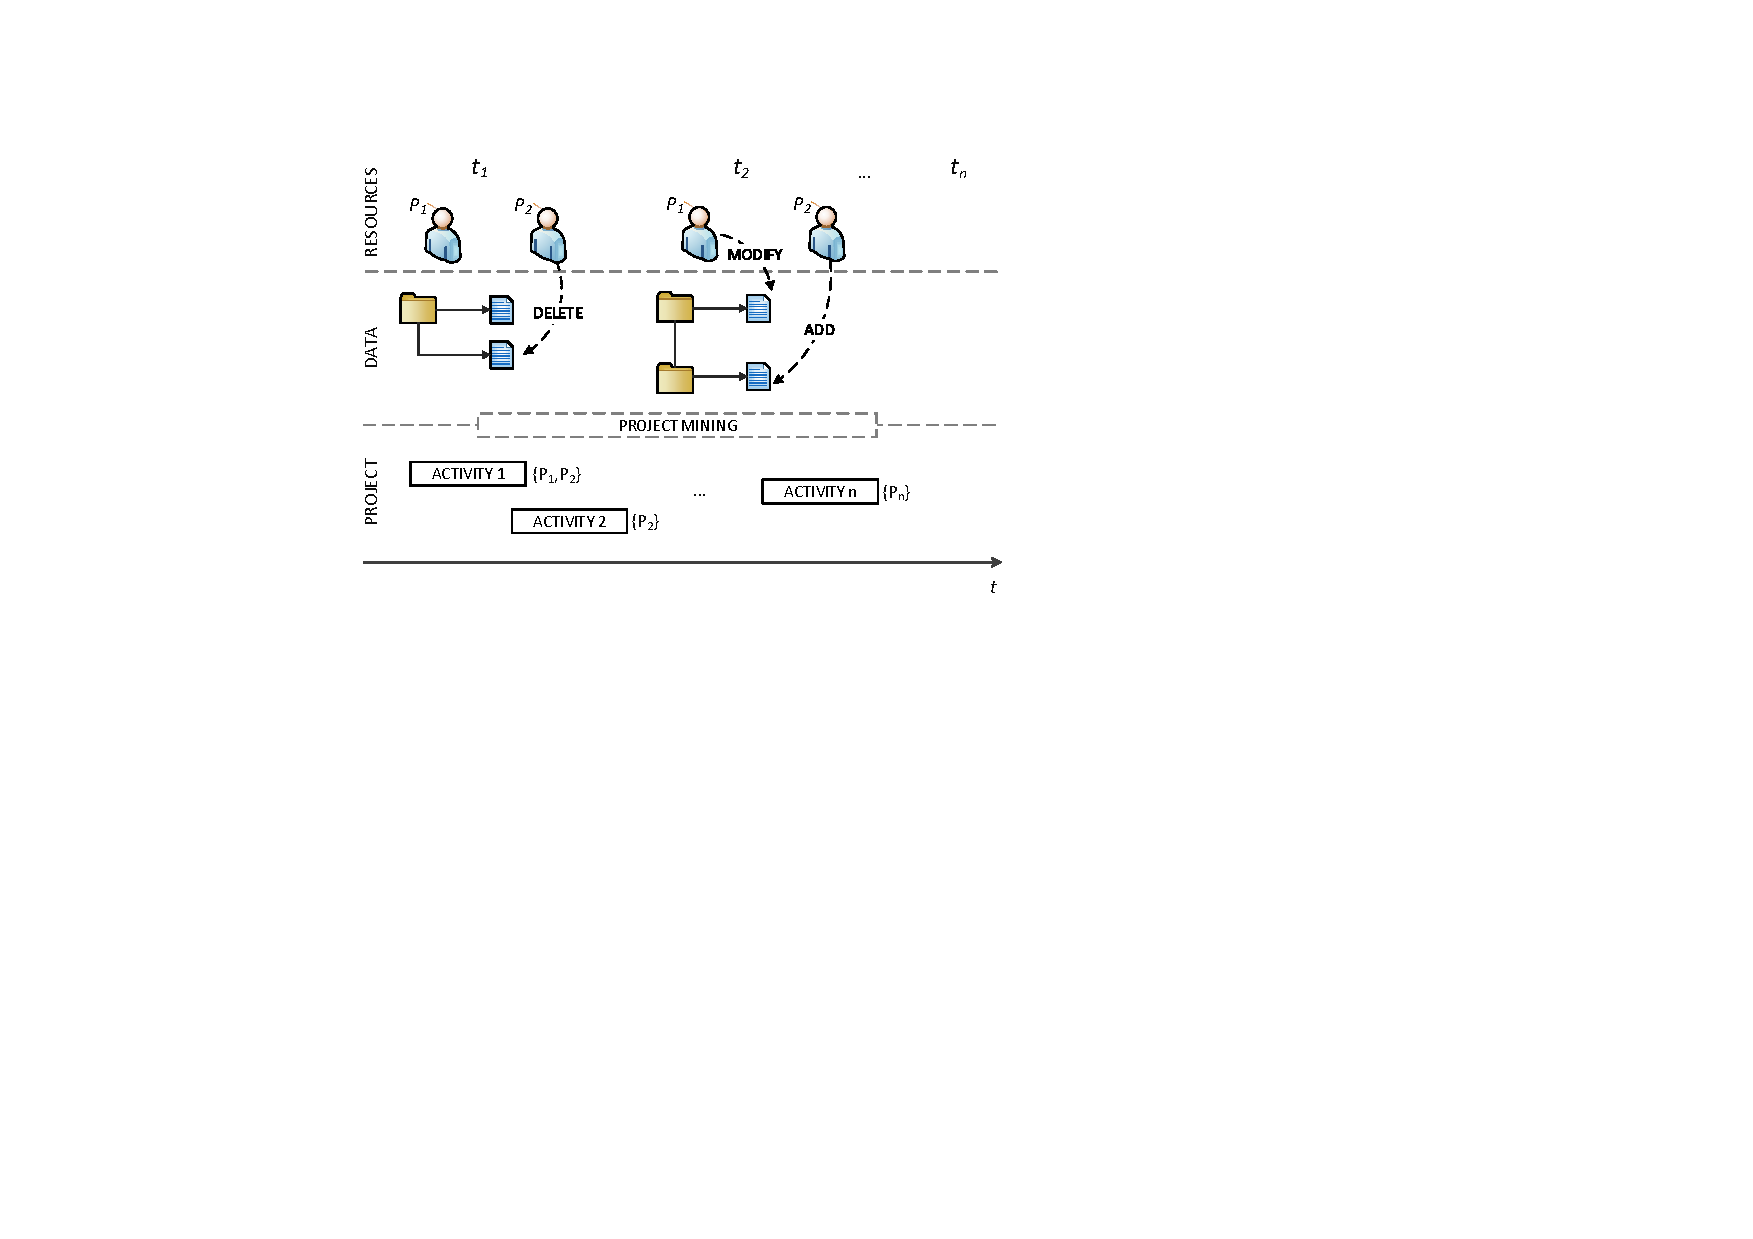
\includegraphics[width=.8\textwidth]{bpm2015/imgs/ProjectMining.pdf}
\caption{Problem illustration}
\label{fig:bpm2015problem}
\end{figure}

Documentation is required not only explicitly as part of some activities but also to comply with norms and regulations that may require some evidence of the actions being performed in the organization. Documents are usually free of format or contain tables, at best. The unstructuredness of data makes it difficult to monitor processes and check rules on them. A starting point for analysis of project-oriented processes can be data logs %generated for  %usually consist of subversion projects
that are stored in Software Configuration Management (SCM) systems that help tracking the evolution of data and restore information if needed~\citep{voinea_open_2006}.
However, hundreds of versions of thousands of files are common in a single project~\citep{voinea_multiscale_2006}, which makes it impractical to browse this data manually.

%We focus on project mining motivated by a real case scenario in the scope of the SHAPE research project\footnote{\url{http://ai.wu.ac.at/shape-project/}}.
%The data log is provided by a Version Control Systems (VCS) whose information is not subdivided into traces related to process instances but consists of a hierarchy of work streams associated with individual files being added, modified or deleted in a subversion repository.

Let us see an example inspired by a real scenario of a process to write a project proposal that uses a Version Control System (VCS) to store the data. The project history, and hence, the data produced, starts when people begin to work on the proposal, which involves a description of the project goals and milestones, a division of tasks into work packages, an estimation of cost and resources required, etcetera. This information is spread in the repository over several folders containing different documents, which are later merged into a single file. If the proposal is accepted, the first step is to organize a kickoff meeting and assign specific resources to the work packages. A hierarchical set of folders is then created in the repository in order to store the information generated for each work package. As the project evolves over time, resources contribute by adding, removing or modifying information to the VCS repository. %\todo{Should answer point 3 on the review-list: Missing concrete examples of the need to “prove compliance to rules and regulations”. Which important rules and regulations will the analysis help comply with?} 
Project evolution is guided by specific norms that impose the execution of predefined steps. For instance, the European norm EN5016 requires a preliminary \gls{ram} analysis to support targets. 
%Data stored in the VCS can be used to prove compliance to rules and regulations of the domain. For instance, in the railway industry, 

Table~\ref{tab:bpm2015example} depicts an excerpt of the log data generated, where the first column (on the left hand side) indicates the commit identifier, the second column indicates the person who committed changes, the third column indicates the commit date, %the fourth column shows (optional) descriptive information to clarify the scope of the changes performed
and the fourth column indicates the files affected and the type of action performed among added (A), modified (M) and deleted (D).
For the sake of simplicity, the table shows the log data of a specific time period and the actions related to a specific task, namely, $\defineExample$. That task was assigned to resource X % after a project meeting. %, when a part of project members asked for a toy example to better understand the problem domain.
and was supervised by resource Y and, later on, also by resource Z.
%An extract from the log concerning this period, that shows some crucial steps in the \emph{example} task, is reported on table \ref{tab:example}. Comments were left out from this representation, since at the current state we don't delve into them.

\begin{table}[bt]
\caption{Excerpt from VCS log data for the referenced time period }
\label{tab:bpm2015example}
%\scriptsize
{
%	\renewcommand{\arraystretch}{1.3}
\centering
%\fontfamily{phv}\fontseries{mc}\selectfont
\begin{tabular}{m{.8cm} m{1.5cm} m{3cm} p{5.8cm}}
%\hline\noalign{\smallskip}
%\hline
\toprule
\textbf{CID}	 & \textbf{Resource} & \textbf{Date} & \textbf{List of changes} \\
%\noalign{\smallskip}
%\hline
%\noalign{\smallskip}
%\hline
\midrule
%\noalign{\smallskip}
\multirow{2}{*}{1} & \multirow{2}{*}{Y} & \multirow{2}{*}{2014-11-12~11:57:46} & A /example \\
& & & A \slash example\slash SHAPE\slash\-ToyStation\-Example.docx \\ \midrule %\hdashline

%\multirow{2}{*}{205} & \multirow{2}{*}{X} & \multirow{2}{*}{2014-11-14 16:26:23} & A /example/ToyStation.bpmn \\
%& & & A /example/ToyStation.png \\ \hline %\hdashline

\ldots & \ldots & \ldots & \ldots \\ \midrule

%\noalign{\smallskip}
\multirow{2}{*}{3} & \multirow{2}{*}{X} & \multirow{2}{*}{2014-11-14 16:34:07} & M /example/ToyStation.bpmn\\
& & & M /example/ToyStation.png \\ \midrule%\hdashline

%\multirow{7}{*}{207} & \multirow{7}{*}{X} & \multirow{7}{*}{2014-11-27 14:18:59} & M /example/SHAPE-ToyStation-Example.docx \\
%& & & D /example/ToyStation.bpmn \\
%& & & M /example/ToyStation.png \\
%& & & A /example/ToyStation\_0Loop.bpmn \\
%& & & A /example/ToyStation\_1Loop.bpmn \\
%& & & A /example/ToyStation\_nLoop.bpmn \\
%& & & A/example/ToyStation\_old.bpmn\\ \hline

%\ldots & \ldots & \ldots & \ldots \\ \hline

%\noalign{\smallskip}
4 & W & 2014-12-15 13:49:11 & D /example/Download \\ \midrule %\hdashline

%\noalign{\smallskip}
5 & W & 2015-01-08 16:06:41 & A /example/Download2\\ \midrule %\hdashline

%\noalign{\smallskip}
\multirow{2}{*}{6} & \multirow{2}{*}{X} & \multirow{2}{*}{2015-01-13 11:47:09} & M /example/ToyStation\_0Loop.bpmn\\
& & & M /example/ToyStation\_nLoop.bpmn \\ \midrule %\hdashline

%\noalign{\smallskip}
\multirow{2}{*}{7} & \multirow{2}{*}{Z} & \multirow{2}{*}{2015-01-16 16:50:29} & A /example/ToyStation\_0Loop.pdf\\
& & & A /example/ToyStation-feedbackZ.pdf\\ \bottomrule %\hdashline
\end{tabular}\\ 
}
\end{table}

%Process mining techniques can help to discover processes from log data.
%Existing process mining techniques can deal very well with execution logs whose data is subdivided into \textit{traces} representing different process instances in which events are easily identifiable (e.g. through a \textit{caseId}).
%Procedural (e.g. BPMN~\citep{bpmn2_stable}, Petri nets~\citep{aalst_application_1998}, EPC~\citep{vanderaalst_formalization_1999}) as well as declarative (e.g. Declare~\citep{VanderAalst2009}, DPIL~\citep{zeising2014towards}) modeling languages can be used to represent the process discovered.
%Once a process model is discovered, it can be checked whether it is compliant with the existing (already known) process model and enhance the model or the way the process is executed accordingly.
%Performance can also be analyzed and compared to the expected values defined by key performance indicators (KPIs)~\citep{delrioortega_definition_2013}.

%\begin{table}[bt]
%\caption{Process mining vs. project mining}\label{tab:processVSprojectmining}
%\centering
%\begin{tabular}{l c c}
%%\hline\noalign{\smallskip}
%%\hline
% ~&~  Process Mining~&~Project Mining\\
%%\noalign{\smallskip}
%\hline
%%\noalign{\smallskip}
%Defined goals~&~  \cmark ~&~ \cmark \\
%Resource~&~ \cmark ~&~ \cmark \\
%Activities/Tasks~&~ \cmark ~&~ \cmark \\
%One time~&~ \xmark ~&~ \cmark \\
%Repetitive~&~ \cmark ~&~ \xmark \\
%\hline \\
%\end{tabular}
%\end{table}

%However, due to the ad-hoc nature of project-oriented business processes, the event logs for these processes look different.
%Therefore, mining of project-oriented business processes needs to be done in a different way.
%Whereas in traditional process mining the main goal is to discover the execution order and relation among activities, project mining aims at discovering the structure of the project along with its temporal progress and information about the actors involved.

% Deviations from the designed plan can then be measured, as well as the fulfillment of milestones, deadlines, resource usage constraints, cost expense, etcetera. Table~\ref{tab:processVSprojectmining} illustrates the main differences between process mining and project mining concepts\todo{CC: I'm not sure whether this table is representative and/or necessary}.


%\begin{table}[bt]
%\centering \begin{tabular}{m{1cm} m{2cm} m{2.8cm} m{3cm} l}
%%\hline\noalign{\smallskip
%\hline
%CID	&	Resource	&	Date	&	Message	&	List of changes \\
%%\noalign{\smallskip}
%\hline
%%\noalign{\smallskip}
%\hline
%\multirow{3}{*}{1} & \multirow{3}{*}{pol@uni.edu} & \multirow{3}{*}{2006-02-17 15:30} & \multirow{3}{*}{} & A /templates \\
%& & & & A /temp/costsplan.doc \\
%& & & & A /temp/proposal.pdf \\ \hline %\hdashline
%\multirow{3}{*}{2} & \multirow{3}{*}{al@co.com} & \multirow{3}{*}{2006-02-19 12:00} & \multirow{3}{*}{Reviewed proposal} & A /slides \\
%& & & & A /slides/review.doc \\
%& & & & M /temp/proposal.pdf \\ \hline %\hdashline
%\multirow{2}{*}{3} & \multirow{2}{*}{al@co.com} & \multirow{2}{*}{2006-02-19 17:05} & \multirow{2}{*}{Renamed a file} & D /temp/proposal.pdf \\
%& & & & A /temp/proposal\_final.pdf \\ \hline %\hdashline
%\multirow{2}{*}{4} & \multirow{2}{*}{jb@uni.edu} & \multirow{2}{*}{2006-02-23 11:05} & \multirow{2}{*}{Added CV} & \multirow{2}{*}{A /skills/CV.pdf} \\
%& & & & \\ \hline %\hdashline
%\multirow{2}{*}{5} & \multirow{2}{*}{ccm@uni.edu} & \multirow{2}{*}{2006-02-19 17:05} & \multirow{2}{*}{WPs description} & A /goals/WPS\_description.doc \\
%& & & & M /temp/costsplan.doc \\ \hline %\hdashline
%\multirow{2}{*}{\ldots} & \multirow{2}{*}{\ldots} & \multirow{2}{*}{\ldots} & \multirow{2}{*}{\ldots} & \multirow{2}{*}{\ldots} \\
%& & & & \\ \hline
%\end{tabular}\\ \hfill
%\caption{A representation of VCS log data}
%\label{tab:VCSlog}
%\end{table}

%\begin{figure}
%\centering
%\includegraphics[height=6.2cm]{imgs/pm-pic}
%\caption{Problem illustration,}
%\label{fig:example}
%\end{figure}

Existing frameworks, such as Subversion or Git, allow to access their logs in different ways. However, the covered information is limited to (roughly) that depicted in Table~\ref{tab:bpm2015example}. Especially for big projects that are frequently updated over a large period of time, these logs are complex to analyze.
Therefore, the problem to address is how to analyze and visualize the information produced in project-oriented business processes such that it can be represented in an understandable and manageable way by project experts and
enable, a.o., the automation of mechanisms for compliance checking.
The following properties of project-oriented process logs must be taken into account to achieve this goal: (i) VCS repositories consist of a hierarchy of folders and files which are logically organized such that work is grouped in a specific way; (ii) process activities are not registered in VCS log entries. Therefore, such information must be inferred by reasoning on the repository structure and/or the content of the log entries; (iii) the granularity of the events is unknown a priori and it needs to be defined before analyzing the data.
%Therefore, the goal of project mining is to represent that data in a way that is natural to the project (i.e., by deriving the project structure and its progress over time) taking into consideration the aforementioned properties of VCS logs.

%\begin{itemize}
%\item we cannot see activities, but we can see that work was done
%\item hierarchical work structure (requirements)
%\item names of activities are not directly explicit
%\item granularity of events (e.g. in our case is on the file level)
%\end{itemize}

%We need to retrospect that the things that we did in the project were complete and correct. Answer to questions like: Did we do all the stuff?\\ \hfill

%Logs carry much more information (such as the number of lines or bytes modified in a file) but for the moment let's treat only this level of granularity.

%\todo[inline]{CC: Some further work is required on sections 2.1 and 2.2 so that the transition from the former to the latter is smooth and the last part of section 2.2 makes sense}


\subsection{Related Work}
\label{sec:bpm2015related}

The problem described has been addressed in the literature from different perspectives. The first category of related work tackles the problem by transforming it into a process mining problem. Consequently, approaches have been developed to preprocess VCS data such that process mining techniques can be applied, and hence, a business process can be derived from the log data.
In this group, Kindler et al. \citep{Kindler2006,kindler2006incremental} developed an algorithm for extracting software processes that are mapped to Petri Nets. Activities, which are not explicit in the logs, are discovered from their input and output artifacts. However, strong assumptions are made on the filenames as well as on the software process lifecycle. %(always design, code, review, testres). Activities (which are not explicit in the logs, like in our case) are discovered from their input and output artifacts. Here defined as triples $<I,O,R>$ where I=input, O=Output, R=resouce who perfomed it.
Rubin et al. in \citep{rubin2007process} addressed the problem of engineering processes that are not well documented and are usually unstructured. They provided a bridge from Kindler et al.'s approach to ProM \citep{van2005prom} in order to mine different process perspectives, such as performance social network analyses. %but not from a project point of view.
Rubin et al. \citep{rubin2014agile} applied process mining to the touristic industry and obtained user processes from web client logs pursuing the goal of improving the software system by analyzing the underlying process.
Poncin et al. \citep{Poncin2011a} developed the FRASR framework for preprocessing software repositories to transform the VCS data to logs that conform to the process mining event log meta model~\citep{van2005meta} as utilized in ProM \citep{van2005prom}.
However, these approaches disregard the single-instance nature of project-oriented business processes and treat them as procedures that can be repeated over time.

The second category of related work focuses on the visualization of VCS data %by defining measurements such as things that can be plotted into a chart.
for different purposes.
%There are two main lines of how this problem was approached in literature.
%\paragraph*{visualization perspective} defining measurements such as things that can be plotted into a chart. But, they haven't any explicit notion of work structure.
%\paragraph*{preprocessing} - VCS data is transformed in order to comply to the process mining meta model from van Dongen and van der Aalst \citep{van2005meta}. This means that they are oriented to discover "classical" processing (i.e. repeated many times in the logs).
Several approaches study the interaction among developers over time from a visualization point of view. For instance, Ogawa and Ma \citep{ogawa2010software} drew storyline pathways to show the story of each developer's contribution. Other approaches analyze and visualize VCS data at file level in order to discover file version evolution. Voinea and Telea~\citep{voinea_multiscale_2006} introduced an interactive navigation method to surf file version evolution as well as two methods to cluster versions of the same file in an abstraction layer. Wu et al.~\citep{jingwei_evolution_2004} also visualized the evolutions of entire projects at file level, emphasizing the evolution moments.
Finally, several approaches study change prediction with the aim of discovering prediction patterns that can help in the process of software development~\citep{zimmermann_mining_2004,ying_predicting_2004}.
%Feld et al. \citep{feldt2013supporting} used software project data to \emph{predict} potential problems during development. Heatmaps, used to visualize source code changes in a two dimensional space, showed to be easily readable also by non experts.
The approaches mentioned in this category as well as others that apply similar techniques~\citep{feldt2013supporting,kagdi_mining_2006,dambros_flexible_2008} focus on studying software evolution from different standpoints. However, the goal pursued differs in all cases from our goal in that they are not interested in discovering projects tasks out of the log data, and hence, they lack an explicit notion of work structure that we need to consider for our purpose.

Our approach combines ideas from both areas, as we aim at identifying tasks like in the approaches that rely on process mining, but we must cluster the data in an appropriate way, for which techniques developed in the approaches that pursue visualization may be adapted or extended.

%----------------
%
%Then explain that, in our work, we don't only want to see what's happening. We want also compliance (which means: did things happen in the right way (as they were allowed to)? Compliance can be provided by Process Mining algorithms... but we cannot apply process mining techniques directly (because they need logs structured in different ways - not svn/git logs). Thus, we need to adopt this strategy. 
%
%\section{Approach to Discover the Time Perspective}
%
%%\section{Mining \acs{VCS} Event Data}
\label{sec:bpm2015concept}
In the following, we first formalize the notions encountered in the project mining setting. Then we develop an approach to acquire a hierarchical overview on the project from a repository perspective.

\subsection{Preliminaries}
\glspl{vcs} are used in projects to ensure reliable collaboration. We build our approach on \gls{vcs}. Typically, the workflow in \gls{vcs} is that people work on files (e.g., text, source code, spread sheets) and commit them to the central repository. Project participants comment on their commits so that other participants can better understand the nature of the changes to the files.

Let \Files be the universe of files. Files are organized in a file tree. Therefore, each file $\file \in \Files$ has one parent file. The only file without a parent file is the root file. We capture this information in the parent relation $\parent : \Files \times \Files$. For example, let $\file_p \in \Files$ be the parent of file $\file_c \in \Files$, then $(\file_p, \file_c) \in \parent$.
The transitive closure on the parent files is given by the function $\ancestor : \Files \rightarrow 2^{\Files}$ that returns the set of files along the path to the root.

When project members did a certain amount of work and want to save their current progress, they commit the changes to the \gls{vcs}.
We define changes on files as the events of interest on the lowest granularity.
\begin{definition}[Event] \label{def:bpm2015events}
Let $\Events$ %  = \Files \times \ChangeOperations \times \Timestamps \times \Comments \times \ChangedAmount$
be the set of events. An event $\event \in \Events$ is a four-tuple $(\file, \changeOperation, \timestamp, \comment)$, where
\begin{compactitem}
  \item $\file \in \Files$ is the affected file of the event.
  \item $\changeOperation \in \ChangeOperations =\lbrace\added$, $\modified$, $\deleted \rbrace$ is the change operation on the file with obvious meaning.
  \item $\timestamp \in \Timestamps = \mathbb{N}_0$ represents a unix time stamp marking the time of the event occurrence.
  \item $\comment \in \Sigma^*$ is a comment in natural language text.
%  \item $\changedAmount \in \ChangedAmount$ is the absolute number of changed bytes in comparison to the previous version of the file.
\end{compactitem}
% Let $\ChangeOperations = \lbrace \added$, $\modified$, $\deleted \rbrace$ be the set of change operations on files, \Timestamps represent unix time stamps, and $\Comments \subseteq \Sigma^*$ be comments in natural language text.
% Events $\event \in \Events$ are tuples of the form .
% \todo{TODO: decide, if we need weights on how much of the files changed.
% Also: what about resources?}
%$\file \in \Files$ is a file, $\changeOperation \in \ChangeOperations$ is a change operation, $\timestamp \in \Timestamps$ is a timestamp, and $\comment \subset \Sigma^*$ is a comment in natural language text.
\end{definition}

For events $\event = (\file, \changeOperation, \timestamp, \comment%, \changedAmount
)$ we overload $\file, \changeOperation, \timestamp$, and $\comment$
%,$ and $\changedAmount$ 
to be used as accessor functions. For example, \file is the function $\file : \Events \rightarrow \Files$ mapping an event to its affected file.

Project participants can commit a number of changes to different files at one step. Therefore, we define the notion of commits as follows.
%\todo{Maybe instead use a reduction of an event like $\event_{|\timestamp}$}

\begin{definition}[Commit]
A commit $\commit$ is a set of events sharing the same time stamp and comment, i.e., $\forall \event, \event' \in \commit: \timestamp(\event) = \timestamp(\event') \wedge \comment(\event) = \comment(\event')$. Additionally, each event in a commit affects different files, i.e., $\forall \event, \event' \in \commit : \event \neq \event' \rightarrow \file(\event) \neq \file(\event')$.
\end{definition}
%\todo{Decide: Do we need the definition Commits at all?}

Usually, it is in the hands of project participants, when they decide to commit changes to the \gls{vcs}. In the extreme case, there could be only a single commit made in a project that adds all files to the repository.
Note that this extreme practice would render the use of a \gls{vcs} obsolete. On the contrary, it is common practice to regularly perform commits in order to securely store work progress and to reduce the chance of conflicts~\citep{pilato2008version,Hou2014}. Conflicts occur, when another participant committed changes to a file that is being committed and can cause extra work.
Based on these insights, we make the assumption that commits are regularly made during work.

Projects are decomposed into work packages. We assume a hierarchical work package structure of a project, such that a work package can have sub work packages. Further, the amount of work in a single work package need not be done in one single time span, but it can be split into several activities. Activities have a start and end time, and subsequent activities can have idle periods in between. Thus, we define projects as follows.
\begin{definition}[Project]\label{def:bpm2015project}
A project \Project is a tuple $(\WorkPackages, \Structure, \Activities, \startTimeFunction, \finishTimeFunction, \MappingFunction)$, where
\begin{compactitem}
  \item $\WorkPackages$ is the set of work packages in the project.
  \item $\Structure \subseteq \WorkPackages \times \WorkPackages$ is the relation that hierarchically decomposes work packages into a tree structure.
  \item $\Activities$ is the set of activities that are conducted in the work packages.
  \item $\startTimeFunction : \Activities \rightarrow \Timestamps$ is the function that assigns a start time to activities. Activities are ordered by their start times.
  \item $\finishTimeFunction : \Activities \rightarrow \Timestamps$ is the function that assigns an end time to activities.
  \item $\MappingFunction : \Activities \rightarrow \WorkPackages$ is the mapping function that maps activities to their corresponding work packages.
\end{compactitem}
\end{definition}

Note that this definition reflects an activity centric view on projects. The definition deliberately omits further dimensions, e.g., costs, resources, risks. The idea is not to capture projects in every detail, but to focus on the work packages of a project to obtain an overview of the work that is being done. %\todo{Question: do we want a full-blown definition on projects? with risks, resources, milestones, stakeholders, \ldots?}
We are interested in when work has been started in a work package, and when work packages have been done. This information can be derived from the activities associated to the workpackages. An obvious assumption is that the work package starts with its first activity, and ends when its last activity is completed.

Based on these notions, we can define the task of \emph{project discovery} as reconstructing the project \Project from a set of low level event data \Events.
In the following, we present an approach to this problem.

% \begin{definition}[Project mining]
% 	Given a set of events \Events, the objective of project mining is to identify:
% 	\begin{compactitem}
% 		\item the set of work packages \WorkPackages in the project.
% 		\item the start \startTimeFunction, and end \finishTimeFunction of the workpackages in \WorkPackages.
% 		\item the hierarchical relation \Structure between work packages.
% 		\item the mapping function \MappingFunction that assigns assigns events to a work package.
% 	\end{compactitem}
% \end{definition}


% Inital definition which we have to align to the current \\
% A commit is a set of change operations. $\commit \equiv \lbrace c \in \changeOperation \rbrace \times \comment$ \\
% A change operation is a set of triples $\changeOperation \equiv \lbrace F, W, O \rbrace $ where $F, W, O$ are respectively the file, the weight (how much a change affected the file), and the operation type ($O={modified,added,deleted}$)\\
% Upon the above sets we can define functions such as a modification function (that, for instance, maps the set of files to their weight), or distance(f1, f2) (but for the moment we don't use it).\\ \vfill

% After the last discussion I identified the following concepts to be formalized. So basically we would need to align the initial definition to was follows.
%
% Definitions: \\
% \begin{definition}[Event]
% Event: something that happens at some point in time. Generally in the past. (Primitive concept: can't be derived from any other concepts? Can it be defined?!)
% Event data: data regarding events. An event over a dataset A is the minimum amount of modification made to the minimum part of A at some point in time. i.e. the smallest possible change.
% \end{definition}
%
% \begin{definition}[Project]
% D2. Project (hierarchy) \\
% a project has a hierarchy. It is a set of event streams. An event stream is an object of the hierarchical structure. (that relates to events).
% \end{definition}
%
% We define a mapping function $f$ from the set of events to objects which is:
% \begin{itemize}
% \item surjective and not injective (i.e. every element in the codomain has a corresponding element if the domain, and it doesn't hold that for two different elements $a, b$ of the domain there exist two different mappings $f(a), f(b)$ in the codomain.
% \item total
% \end{itemize}
%
% Function $f$ partitions the set of events...
% \begin{definition}[Commit]
% A commit is a "bundle" of events.\\
% \end{definition}

% \begin{definition}[Drill]
% Here we formally define the agglomeration feature. We can drill-up and drill-down on the data. E.g. show grouped events for folders at different levels.
% \end{definition}

\subsection{Time Perspective Discovery}\label{sec:subsec:discovery_technique}
\begin{figure}[b]
\centering
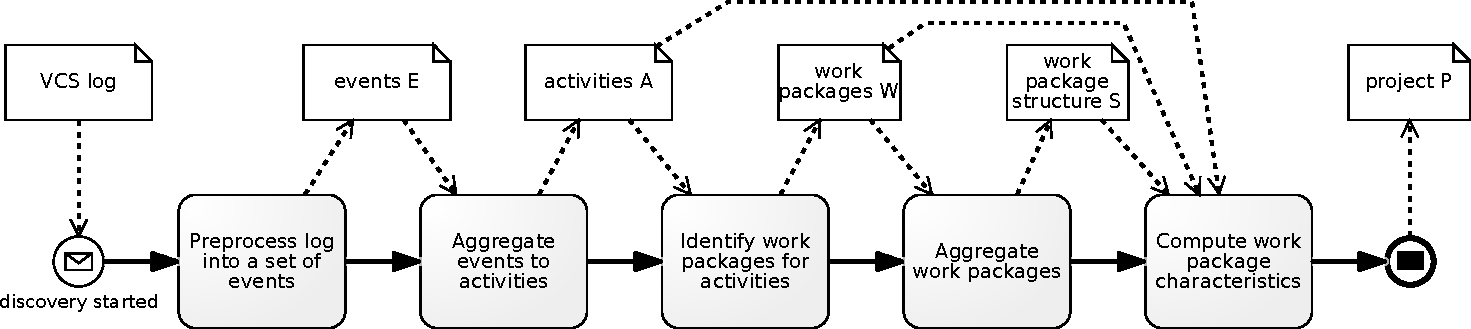
\includegraphics[width=\textwidth]{bpm2015/imgs/Project_discovery}
\caption{Project discovery technique overview as BPMN process model.}
\label{fig:project_discovery_technique}
\end{figure}
For project discovery from the \gls{vcs} commit history, we need to identify activities that are performed, associate the activities to work packages and recreate the work package structure of the project.
Our aim is to create a hierarchical model that provides an overview of the project work.
Therefore, we have to identify the start and end times of activities and of work packages before we can visualize the project work. The input to the technique is the log that is stored in the \gls{vcs}. The challenge is that the raw log only records commits on the file system level and information on activity level is missing. However, we can deduce activity information from events based on the following assumptions.

\begin{itemize}
  \item \textbf{A1: Meaningful file tree structure.} The file tree structure in a project represents its work package structure. That is, the knowledge workers organize their work in a file hierarchy that reflects the project structure.
  \item \textbf{A2: Local changes.} Activities in a work package affect only files of the work package folder, or in the corresponding sub-tree in the file tree structure.
  \item \textbf{A3: Frequent commits.} Commits to the \gls{vcs} are regularly performed, when conducting work in an activity.
\end{itemize}

Note that assumption A1 can be seen as a strong assumption on the file tree structure. Nevertheless, we argue that even if A1 is not entirely met, the aggregation of work information on the file tree hierarchy provides a valuable view on the project.
Figure~\ref{fig:project_discovery_technique} shows the different steps of the technique. We describe each of them in detail.

\subsubsection*{Step 1: Preprocessing.} The first step is to transform raw logs of version control systems (which might be grouped by commits) into a list of events as specified in Definition~\ref{def:bpm2015events}. This step is easily done by replicating the information on commit level to be contained in the events. The output is a set of events \Events.

\subsubsection*{Step 2: Aggregating events to activities.}
Given the set of events \Events that we gathered from a version control system, the next step is to identify the activities to which the events belong. Note that we do not know the activities of the project in advance, but need to infer them based on the events. Each event affects a single file in the file hierarchy.

\begin{figure}
\centering
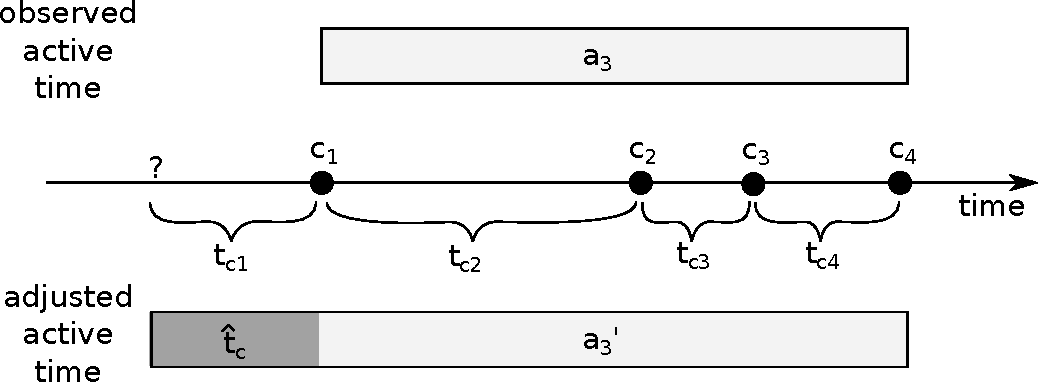
\includegraphics[width=.7\textwidth]{bpm2015/imgs/activity_adjustment}
\caption{Adjustment of activity start time \startTimeFunction. }
\label{fig:activity_adjustment}
\end{figure}

Based on assumption A2, we are interested in activities conducted in a work package, that is, we filter for the events that are contained in the given file or its children. For every file $\file$ of interest, we select the set of events affecting the file or its children as $\Events_{\file} = \lbrace \event \in \Events \mid \file = \file(\event) \vee \file \in \ancestor(\file(\event))  \rbrace$. The task is then to find the activities which emitted the set of events $\Events_{\file}$. We rely on assumption A3, which states that during an activity, we expect multiple commits. Assumption A3 allows us to conclude that if we do not observe commits for a longer period of time, there is no activity being performed in the work package.

%To derive coarse grained activities from low level events, clustering techniques~\cite{Berkhin2006ClusteringSurvey}, or abstraction functions~\cite{baier2014bridging} can be used.
%Former assume that a distance function measures the distance between events, and partitions the set of events into groups. Well-known examples are the k-means clustering~\cite{Berkhin2006ClusteringSurvey}, or hierarchical agglomerative clustering.
To this end, we adopt the abstraction technique by \citep{baier2014bridging} and allow the domain expert to formulate rules for aggregating events to activities based on boundary conditions. Assuming that people frequently commit their progress (A3), we can specify a boundary condition based on the temporal distance to previous events. For example, we can specify that a time period of seven days without a commit is a boundary condition. %But also other boundary conditions can be selected, e.g., based on resources.
As the result, we obtain the mapping from events to these activities, which we call $\eventMapping_{\file} : \Events_{\file} \rightarrow \Activities_{\file}$ in the remainder of the paper. The set of discovered activities identified for the work package based on given boundary conditions is then $\Activities_{\file} = \lbrace \activity \mid \event \in \Events_{\file}, \eventMapping_{\file}(\event) = \activity \rbrace$. We also define the inverse mapping, that is, the mapping from an activity to its events as $\eventMapping_{\file}^{-1} : \Activities_{\file} \rightarrow 2^{\Events_{\file}}$.

With the events mapped to activities, we need to find the temporal boundaries of the target activities. That is, we define the functions $\startTimeFunction$ and $\finishTimeFunction$ for each activity. The challenge here is that we do not know when an activity actually started, because the start of the activity is not recorded in the \gls{vcs}. We can only observe the time of the first commit in that activity, but commits usually mark progress of an already running activity.

To address the challenge of missing start times, we impute the missing start time by prepending the expected active time $\expectedActiveTime$ before a commit, as illustrated by Figure~\ref{fig:activity_adjustment}. This notion assumes that project participants commit their work progress after a certain amount of time. However, we cannot compute \expectedActiveTime by looking at the average commit rate in a work package, because this average is based on busy periods and idle periods. We need to factor out the idle periods in the computation of this measure.
%Therefore, we use the following formula.
%Let $\file$ be a file in the file tree that represents a work package, and let $\Events_{\file}$ be the corresponding events for all the children of $\file$. Let further $\Activities$ be the activities identified for the work package based on given boundary conditions.
We know the end time of the activities, as the last commit marks the completion of work. Therefore, each activity \activity based on given boundary conditions has the associated end time $\finishTimeFunction(\activity) = \max(\lbrace \timestamp(\event) \mid \event \in \eventMapping_{\file}^{-1}(\activity)  \rbrace)$. Further, we write the first event's timestamp of an activity as the function $\startTimeFunction'(\activity) = \min(\lbrace \timestamp(\event) \mid \event \in \eventMapping_{\file}^{-1}(\activity)  \rbrace)$.
Then, we define $\numCommits:\Activities_{\file} \rightarrow \naturalNumbers$ as the number of commits in one activity, formally $\numCommits(a)=|\lbrace \commit \mid \event \in \commit \wedge \eventMapping_{\file}(\event)=a\rbrace |$.

With this information the expected active time between commits \expectedActiveTime is given as follows.

\begin{equation}
	\expectedActiveTime = \frac{\sum_{\activity \in \Activities_{\file}} \left(\finishTimeFunction(a) - \startTimeFunction'(a)\right)}{\sum_{\activity \in \Activities_{\file}} (\numCommits(\activity)-1) }
\end{equation}

We assume that there is at least one activity spanning over at least two commits, i.e., $\exists \activity \in \Activities_{\file} \mid \numCommits(\activity) > 1 $. Translated to our boundary condition, this assumption is that there is at least one week in each work package, in which there were at least two commits made. Otherwise, we set $\expectedActiveTime$ to 0 for the current file \file due to lack of information.

Given the expected active time between commits $\expectedActiveTime$, we can finally adjust the start time of each activity. Therefore, we set the associated start time for each activity as $\startTimeFunction(\activity) = \startTimeFunction'(\activity) - \expectedActiveTime$. That is, we subtract the expected active time from the first commit's timestamp.

We apply Step 2 to all files $\file$ in the file tree to get $\Activities_\file$. For the remainder of this paper, we define the function $\fileToActivity : \Activities \rightarrow \Files$ that contains the mapping information of the discovered activities to their originating files. Finally, we set the activities \Activities in the project to be the union of the activity sets per file $\bigcup_{\file \in \Files} \Activities_\file$.

% \begin{definition}[Abstraction Function]
% Formally, we rely on an abstraction function $\abstractionFunction : 2^{\Events} \rightarrow 2^\Activities$ that maps a set of events to a set of activities.
% \end{definition}
%
% The abstraction function \abstractionFunction operates on a set of events


\subsubsection*{Steps 3 and 4: Mapping activities to work packages and aggregating.}
Once activities have been identified, we want to climb to the next abstraction layer: the work packages. Assumption A1 allows us to specify a one-to-one mapping $\kappa : \Files \rightarrow \WorkPackages$ between files in the file tree structure and work packages. More precisely, we construct the set of work packages $\WorkPackages$ isomorphic to the set of files $\Files$, such that the $\parent$ relation is preserved in the work package structure \Structure relationship. %This way, we assign the discovered activities of a selected file $\file'$ to the work package corresponding to $\file'$.

The mapping $\MappingFunction$ of activities to work packages is simply $\MappingFunction(\activity) = \kappa (\fileToActivity(\activity))$. That is, the corresponding work package of the activity that was discovered for a file.
%The aggregation of work packages is done according to the hierarchy obtained from the file tree structure.
In this way, we provide an activity based view on work packages, and we can aggregate on each level in the file system to see active periods of the corresponding hierarchy level.


\subsubsection*{Step 5: Computing work package characteristics.} In this final step, we compute measures of interest for the discovered work packages. First, we obtain the temporal boundaries of a work package by the functions $\startTimeFunction$ and $\finishTimeFunction$ of the associated activities.

Let $\MappingFunction^{-1} : \WorkPackages \rightarrow 2^{\Activities}$ be the inverse of the mapping function $\MappingFunction$ of the project.
The start and end time of a work package ($\startTimeFunction_{\WorkPackages}$ and $\finishTimeFunction_{\WorkPackages}$) are functions from work packages to timestamps. The start time is defined as $\startTimeFunction_{\WorkPackages}(\workPackage) = \min(\lbrace \startTimeFunction(\activity) \mid \activity \in \MappingFunction^{-1}(\workPackage)\rbrace )$, and the end time function of work packages $\finishTimeFunction_{\WorkPackages}$ is analogously defined using the maximum of the end times $\finishTimeFunction(\activity)$ of the activities.
We call the duration of a work package $\durationOfWorkPackage$ that is the difference between $\finishTimeFunction_{\WorkPackages}$ and $\startTimeFunction_{\WorkPackages}$.

Moreover, we are interested in the ratio of active working periods (i.e., the time spans of activities) to the total work package duration. This quantity helps to estimate the average work intensity in a work package.

\begin{definition}[Coverage]
The coverage \coverage of work packages by activities is a function $\coverage : \WorkPackages \rightarrow [0,1]$ and is defined as follows.
\begin{equation}
\coverage(\workPackage) = \frac{\sum_{\activity \in \MappingFunction^{-1}(\workPackage)}  \left(\finishTimeFunction(a) - \startTimeFunction(a)\right)}{\durationOfWorkPackage(\workPackage)}
\end{equation}

\end{definition}

With this final step, we lifted the information hidden in low level events to a high-level Gantt chart perspective, with which project managers are familiar. In the following, we compare our technique to existing process mining approaches.


% Here, we present a first approach to project mining that serves to offer a rough estimation on the work packages and their structure in a project.
% The proposed approach in this paper builds on the assumption that the file structure in the project repository is meaningful.
%
% %We acknowledge that this assumption might not be valid in all cases, but we shall demonstrate the usefulness of the approach
%
% Based on this assumption, the main task of project mining is to identify activities that are performed and map them to the work packages of the project.
%
%
%
% The approach is based on the general assumption that there is a \emph{distance} between events and we can algorithmically measure it.



% Technique: \\
%
% Algorithm (from VCS to project) \\
% \begin{verbatim}
% pseudocode of the algorithm
% \end{verbatim} 
%
%\section{Evaluation}\label{sec:bpm2015evaluation}

In this section we evaluate our solution to the project mining problem, and show results for the example presented in Section~\ref{sec:bpm2015background}.

\subsection{Experimental setup}

%
%This section should clarify the objective of the evaluation. What do we try to study with the evaluation (which quality characteristics)? This also relates to the question whether we let the result speak for itself or if we benchmark with competing approaches. here, you should also mention that the technique was implemented as a prototype.

We evaluate our technique by a visual perspective and by comparison to possible different approaches. To this end we implemented our technique as a prototype. We used JAVA as a programming language to code the logic of our technique. For the visualization part we made use of custom SWT widgets provided by the Nebula Project\footnote{https://www.eclipse.org/nebula/}. Our program can deal with logs from Subversion (SVN) \cite{pilato2008version} and Git\cite{torvalds2010git}, but it can be extended to other version control systems by providing an implementation of the preprocessing step discussed in Section~\ref{sec:subsec:discovery_technique}.
We ran the software in an Intel\textregistered Core \texttrademark~i5-4570 CPU @ 3.20 GHz x 4 machine with 15.6 GiB of RAM and Linux kernel 3.13.0-46-generic 64-bit version.

\subsection{Input data description}

We tested our prototype with real-world log data taken from the SHAPE project. Logs were exported from the SVN and Git repositories of different projects. They come from the railway domain and describe engineering processes. Documentation stored in the repositories consists of manually produced text files, diagrams, and files coming from proprietary tools that are typically used in the domain.

We will display results for the SVN log that describes the process oriented project for SHAPE. Data span over one year, going from January 2014 to January 2015. This time window covers the phases of project definition and planning, and a part of the project execution. In the first phase, feasibility of the project was studied and budget, schedule and resources were determined. Proposal submission marked the end of this phase. The second phase started with a kickoff meeting in October 2014 and is still ongoing.

The total number of participants who actively contributed to the work packages stored in the SVN repository was 8 people in the beginning, with new resources joining the project after the kickoff date. The total number of files and directories counts up to 156 objects and 226 overall commit events. The total number of extracted change events after preprocessing (i.e. atomic changes on all the files) was 453.

The last part of the log data contains the task \defineExample, introduced in Section~\ref{sec:bpm2015problem}. For our showcase we assume that this task is contained in a work package named \emph{example}.

\subsection{Output data}

To monitor the project execution, we visualize the work progress that was done for each work package. Monitoring is performed by managers who want to have an overview on the project (which work packages are done, when and for how long, and where idleness or congestion occurs). Gantt charts offer a graphical representation for displaying schedules and jobs that were done on the various work packages \cite{wilson2003gantt} in a way that can easily be communicated to managers.

\begin{figure}
\centering
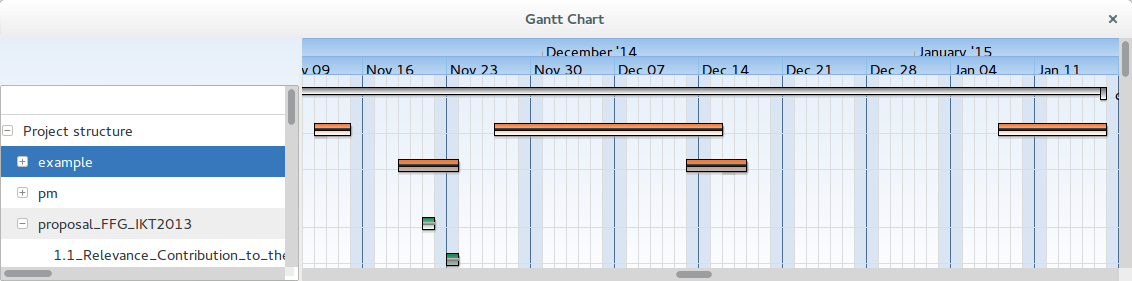
\includegraphics[width=\textwidth]{bpm2015/imgs/aggregation_and_not}
\caption{Data representation from our tool. Atomic events are drawn as dot with a minimal duration and different color per commit. }
\label{fig:example-screenshot}
\end{figure}

Figure~\ref{fig:example-screenshot} is a screenshot of how our tool presents the data. The tree structure on the left represents the \parent relation in the file tree. Events belonging to the same commit have the same color. On the top part of the chart we can see the result of merging events to activities with our aggregation method. Here we have merged the events of the example scenario on their highest abstraction level. The chart shows the three main activities and the idle times between them. %It is possible now to have an overview of the three main active periods in the work package.
On the other hand, in correspondence to expanded directories we show only their status before the aggregation. That is, every time a directory is fully expanded we apply a disaggregation into the corresponding activities. In this way, we can also show the finest granularity of work, i.e. the atomic events.

\subsection{Project Analysis}
Next, we apply our algorithm to the example case from Table~\ref{tab:bpm2015example} and check how it helps to identify work packages. The data is aggregated according to our threshold of seven days. We can observe three groups of events being temporally close to each other according to our threshold. That is, we expect the event data to be grouped into three activities.

The second step of our algorithm takes care of adjusting the starting time of the activities. Furthermore, we vertically order the events and activities in the Gantt chart according to the directory structure to show the mapping from the objects on the Gantt chart to each work package in the tree structure. The last step, computing work package characteristics is done automatically when we collapse a node on of tree.

\begin{figure}
\centering
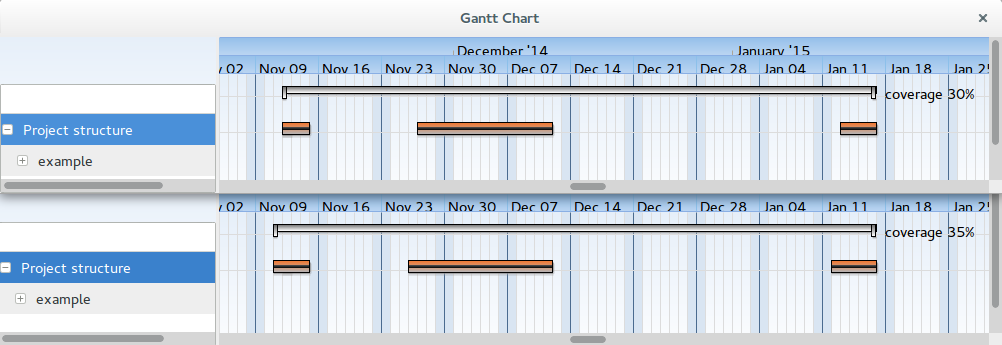
\includegraphics[width=\textwidth]{bpm2015/imgs/coverage_before_and_after}
\caption{Before and after the prepending the expected time before commit. Coverage factor increases when we adjust the starting times of the activities.}
\label{fig:example-collapsed}
\end{figure}

Figure~\ref{fig:example-collapsed} shows a comparison of the case when we do not implement the activity adjustment to the case which adjusts it. In the upper part, activity boundaries are based only on the first commit time that we see in the data. In the lower part, we observe that the start times were adjusted by approximately one day. The tool automatically adjusted the start time of the activities. As a consequence, the coverage factor increases because we expect that there was more work than what we observe by only considering the first commit time.

\subsection{Coverage tests on available open projects}

Finally, we apply our approach on different input data from open source projects. We are interested in exploring how the coverage factor varies in different existing projects. Hence, we take the work package $\workPackage$ as our controlled variable and set it to the highest level of aggregation. Then, we analyze each project of the data set and observe the dependent variable $\coverage(\workPackage)$.
Another variable of interest is the $\expectedActiveTime$ since it gives an idea of the average work speed (commit frequency) during active times.

\begin{table}
\caption{Coverage results for different open source projects}
\label{tab:experiments}
\centering
\begin{tabular}{rcccccc}
%\hline\noalign{\smallskip}
\toprule
\textbf{Log} ~&~ \textbf{Duration} ~&~ \textbf{Idle periods} ~&~ \textbf{Files} ~&~	 \textbf{Commits} ~&~	\textbf{$\expectedActiveTime$} ~&~ \textbf{$\coverage(\workPackage)$}\\
File name ~&~ Days ~&~ Number ~&~ Number ~&~ Number ~&~ Hours ~&~ \% \\ \midrule
%\hline \hline
%\noalign{\medskip}
MiningCVS &	24 & 0 & 89  &	 63 & 9 & 100 \\
%\hline

Whitehall & 1279 & 6 & 6539  &	15566 & 2 & 95 \\
%\hline

Petitions &	834 & 17 & 1562  &	914 & 13 & 59 \\
%\hline

Study &	624 & 13 & 7501  &	736 & 11 & 58 \\
%\hline

The Guardian &	1667 & 59 & 12889  &	 621 & 30 & 44 \\
%\hline

Book &	414 & 15 & 154  & 592 & 5 & 32 \\
%\hline

Papers &	 1859 & 55 & 1791  &	 649 & 20 & 30 \\
%\hline

Requirements & 771 & 22 & 505  &	231 & 17 & 21 \\
%\hline

Yelp &	206 & 6 & 24  &	54 & 20 & 20 \\
%\hline

Adobe &	1076 & 13 & 356  &	237 & 24 & 15 \\ \bottomrule
%\hline

\end{tabular}%\\ \hfill
\end{table}

%We test our tool on log data from open source projects that we find available on the web and data from SHAPE.
The data we used stems from the following projects. \emph{MiningVCS} is our tool. It consists of daily commits and was developed over 24 days.
\emph{Whitehall} is the code name for the Inside Government project, which aims to bring Government departments online in a consistent and user-friendly manner. \emph{Petitions} is a Drupal 7 code base used to build an application on "We The People", the platform to create and sign petitions of the White House.
\emph{Study} is an SVN log about Healthcare domain, taken from SHAPE.
\emph{The guardian} is the log data from the Git repository of the well-known British national daily newspaper.
\emph{Book} is the log data that describes the writing of the book Crypto 101 by Laurens Van Houtven, taken from Git.
\emph{Papers} is taken from SHAPE project for building a paper archive. %Reflects the history of collecting knowledge.
\emph{Requirements} log data is taken from the the Git repository of OpenETCS and belongs to the railway domain.
\emph{Yelp} is the main Github page of Yelp were they showcase all their projects.
\emph{Adobe} is the Adobe Github Homepage v2.0, which is a central hub for Adobe Open sources projects.

Table~\ref{tab:experiments} shows our experiments on the above-mentioned logs and the corresponding coverage factors. Projects that score a high coverage factor are characterized by continuous work. This can be further seen by looking at their average idle times $\avgIdleTime$. Let $n_c$ be the number of commits per work package. We compute the average idle time as follows.
\begin{equation}
\avgIdleTime = \frac{\durationOfWorkPackage  - n_c \cdot \expectedActiveTime }{n}
~,~ n>0
\end{equation}
where $n $ is the number of idle times in the work package. If $n=0$, then we trivially assign $\avgIdleTime = 0$, because there were no break periods over time.

Applying the formula to the above projects, we can observe how projects with a higher coverage factor have actually low values of $\avgIdleTime$. For instance, \emph{Whitehall} scores a $\avgIdleTime$ of 11 days, whereas \emph{Adobe} scores a $\avgIdleTime$ of 36 days.
This supports the usage of the coverage factor $\coverage$ as an indicator for work package time utilization. 
%
%\section{Discussion}
\label{sec:bpm2015discuss}

In this section we compare our method to other alternatives for mining data out of logs and interpret our results.

Well known tools that are used in academia and practice include ProM\cite{van2005prom} and Disco\footnote{http://fluxicon.com/disco/}. Both tools require input data to be in the XES~\cite{Verbeek2011} format. Thus, we convert our data from the $\defineExample$ case into XES. To show events per objects of the project structure, we choose the file path as the \emph{caseId}. To flatten the logs we extract all the file paths and build a mapping from each file to the set of changes done to it.

Figure~\ref{fig:dottedchart} depicts the results of the Dotted chart plugin of ProM applied to our log data. Also here, we observe different changes of each file of the repository. While the files and their corresponding events are shown, the plugin does not allow to rearrange the data in order to understand the file structure, nor does it allow to perform any kind of aggregation or connection between data, to observe them from a higher level perspective.

Figure~\ref{fig:discochart} shows the results from mining our log data with the Disco tool. Here we can see a plot that displays the events that happen over time. The plot has some peeks in correspondence to active times of the \emph{example} work package. They can be grouped in three clusters: an initial cluster with a few amount work, an intermediate cluster with the most significant part of the work, and a final cluster that again is not very active. In this way, clusters can be associated to activities. As a drawback, when the number of work packages and activities increase, the number of peeks grows and generate identifying clusters of activities by look at active (or idle) times becomes unworkable.

\begin{figure}
\centering
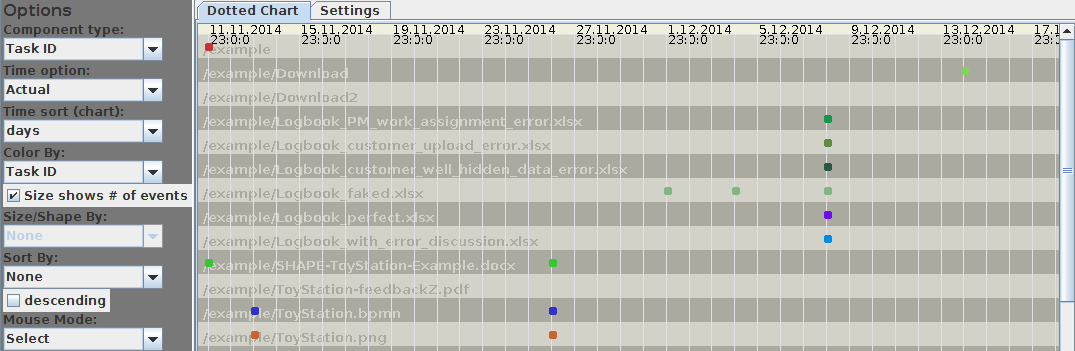
\includegraphics[width=\textwidth]{bpm2015/imgs/dotted_chart_ordered_by_taskID_cut}
\caption{Dotted chart from ProM}
\label{fig:dottedchart}
\end{figure}


\begin{figure}
\centering
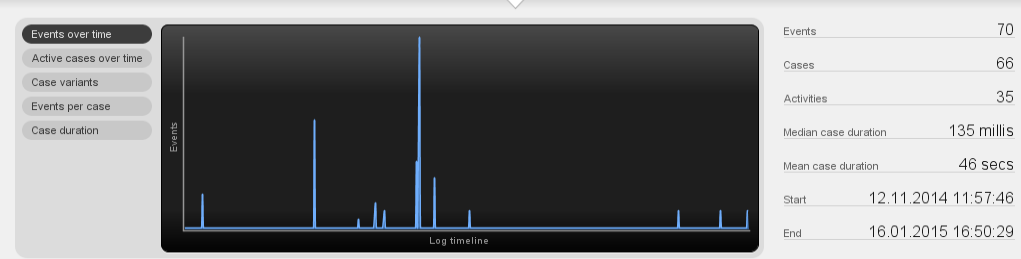
\includegraphics[width=\textwidth]{bpm2015/imgs/disco_screenshot_chart}
\caption{Chart from Disco plotting the events over time.}
\label{fig:discochart}
\end{figure}

Our approach to mining the work progress of project-oriented business processes complements these techniques with metrics and a corresponding visualization that is informative to managers.
%
%\section{Summary}
\label{sec:bpm2015outro}

In this chapter we
%identified a new a class of business processes that are executed according to planned data, resources and time constraints, to achieve predefined goals. We
addressed the problem of mining and visualizing project-oriented business processes in a way that is informative to managers. We define an approach that takes VCS logs as input to generate Gantt charts.
%provided a formal description to capture the project-oriented class of business processes. We presented an approach to mine them as Gantt charts from VCS logs.
Our algorithm works under the assumptions that repositories reflect the hierarchical structure of the project, each work package is contained in a corresponding directory and project members commit their work regularly during active working times.
The approach was implemented as a prototype and evaluated based on real-world data from open source projects.
%We implemented our method as a prototype tool that can visualize the project hierarchy along with events and activities for each level, by aggregation or disaggregation.
%Compared to classical process mining, our method offers a better overview on project structure and on the characteristics of work packages.
%Tests on real-world data, both from open source projects and from SHAPE, show how our metric on work packages can help to better understand work how efficiently they utilize their time.

In future work, we aim to extract further details of the VCS logs in order to calculate metrics that approximate the work effort. %\todo{Point 4 on the reviews: Add a discussion on how the project mining approach can is affected by different projects characteristics: number of commits, number of files, number of activities, duration of the project, number of participants, etc. } 
We plan to investigate on how the project mining approach is affected by project characteristics. Furthermore, we want to utilize statistical methods to better estimate the boundaries of the activities and work packages. Finally, we have already incorporated feedback from managers and plan to extend these to full user studies.

%from a more granular perspective, looking also into the parts of a file that were affected by a change. We also want to investigate ways that help us to better understand the boundaries of activities and work packages. We take into account using natural language processing techniques on the comments associated to commits and analyze their semantics. Furthermore, we want to consider clustering techniques in order to relax our assumptions on the directory structure.


{\bfseries \Large Authors:}

\noindent Saimir Bala, Cristina Cabanillas, Jan Mendling, Andreas Rogge-Solti, and Axel Polleres \hfill

\bigskip

{\noindent\bfseries \Large Published in: \medskip}

\noindent Business Process Management - 13th International Conference, BPM 2015, Innsbruck, Austria, August 31 -- September 3, 2015, Proceedings

\bigskip

{\noindent\bfseries \Large Abstract: \medskip}


\noindent Large engineering processes need to be monitored in detail regarding when what was done in order to prove compliance with rules and regulations. A typical problem of these processes is the lack of control that a central process engine provides, such that it is difficult to track the actual course of work even if data is stored in version control systems (VCS). In this paper, we address this problem by defining a mining technique that helps to generate models that visualize the work history as GANTT charts. To this end, we formally define the notion of a project-oriented business process and a corresponding mining algorithm. Our evaluation based on a prototypical implementation demonstrates the benefits in comparison to existing process mining approaches for this specific class of processes.


\pagebreak

%\todo[inline]{
%	Make cover page. Example:
%	This chapter presents the central research results, which relate to methods and
%	techniques for quantifying inconsistency in business rule bases, pin-pointing elements
%	responsible for the overall inconsistency, and resolving inconsistency. The
%	results and their interrelations are also summarized in a concluding discussion.
%	As stated in the disclaimer, the following results have already been published
%	in various works. Subsequently, the following section includes many materials of
%	these works, which are cited accordingly. All original material was written by
%	myself, except if explicitly stated otherwise.
%}


%\begin{abstract}
Large engineering processes need to be monitored in detail regarding when what was done in order to prove compliance with rules and regulations. A typical problem of these processes is the lack of control that a central process engine provides, such that it is difficult to track the actual course of work even if data is stored in version control systems (VCS). In this paper, we address this problem by defining a mining technique that helps to generate models that visualize the work history as GANTT charts. To this end, we formally define the notion of a project-oriented business process and a corresponding mining algorithm. Our evaluation based on a prototypical implementation demonstrates the benefits in comparison to existing process mining approaches for this specific class of processes.
\keywords{process mining, projects, project mining, version control systems}
\end{abstract} 

\section{Introduction}
Business process management plays an important role for improving the performance and compliance of various types of processes. In practice, many processes are executed with clear guidelines and regulatory rules, but without an explicit centralized control imposed by a process engine. In particular, it is often important to exactly know when which work was done. This is, for instance, the case for complex engineering processes in which different parties are involved. We refer to this class of processes as project-oriented business processes.

Such project-oriented business processes are difficult to control due to the lack of a centralized process engine. However, there are various unstructured pieces of information available to analyze and monitor their progress. One type of data that are often available these processes is event data from version control systems (VCS). While process mining techniques provide a useful perspective on how such event data can be analyzed, they do not produce output that is readily organized according to the project orientation of these processes.

In this paper, we define formal concepts for capturing project-oriented processes. These concepts provide the foundation for us to develop an automatic discovery technique which we refer to as \emph{project mining}. The output of our project mining algorithm is organized according to the specific structure typically encountered in project-oriented business processes. With this work, we extend the field of process mining towards the coverage of this specific type of business process.

The paper is structured as follows. Section~\ref{sec:background} describes the research problem and summarizes insights from prior research upon which our project mining approach is built. Section~\ref{sec:concept} defines the preliminaries of our work and presents an algorithm to mine project-oriented business processes. Section~\ref{sec:evaluation} describes the implementation of this algorithm and discusses the results from its application to VCS logs from a real-world engineering project. Section~\ref{sec:discuss} highlights the implications of this work before Section~\ref{sec:outro} concludes. 
\section{Background}
\label{sec:bpm2015:background}

Here, we describe the addressed problem and related work.


\subsection{Problem Description}\label{sec:bpm2015:problem}
The class of processes that we discuss in this paper are long-term engineering projects. These processes have specific requirements for monitoring. First, they are executed only once according to the specific needs of a particular project, and only partially according to recurring process descriptions. Second, they involve various actors that typically document their work in a semi-structured way using text and tables. Third, work in the project is usually subject to constraints regarding the start and end and the temporal order. Fourth, there is typically no process engine controlling the execution. Fifth, even though these limitations in terms of traceability exist, there are usually strong requirements in terms of tracking when which work was conducted.

%Unlike other types of business processes, the processes we consider here
%representing such projects are specifically tailored to customer needs the specific needs of the project, and there is

In line with these observations, a \textit{project-oriented business process} can be defined as an ad-hoc plan that specifies the tasks to be performed within a limited period of time and with a limited set of resources for achieving a specific goal. Unlike repetitive business processes for which notations such as BPMN~\cite{bpmn2_stable} or EPC~\cite{vanderaalst_formalization_1999} are commonly used, project-oriented business processes may be properly represented with PERT or GANTT models. The concept is illustrated in Fig.~\ref{fig:problem}.


\begin{figure}[tb]
\centering
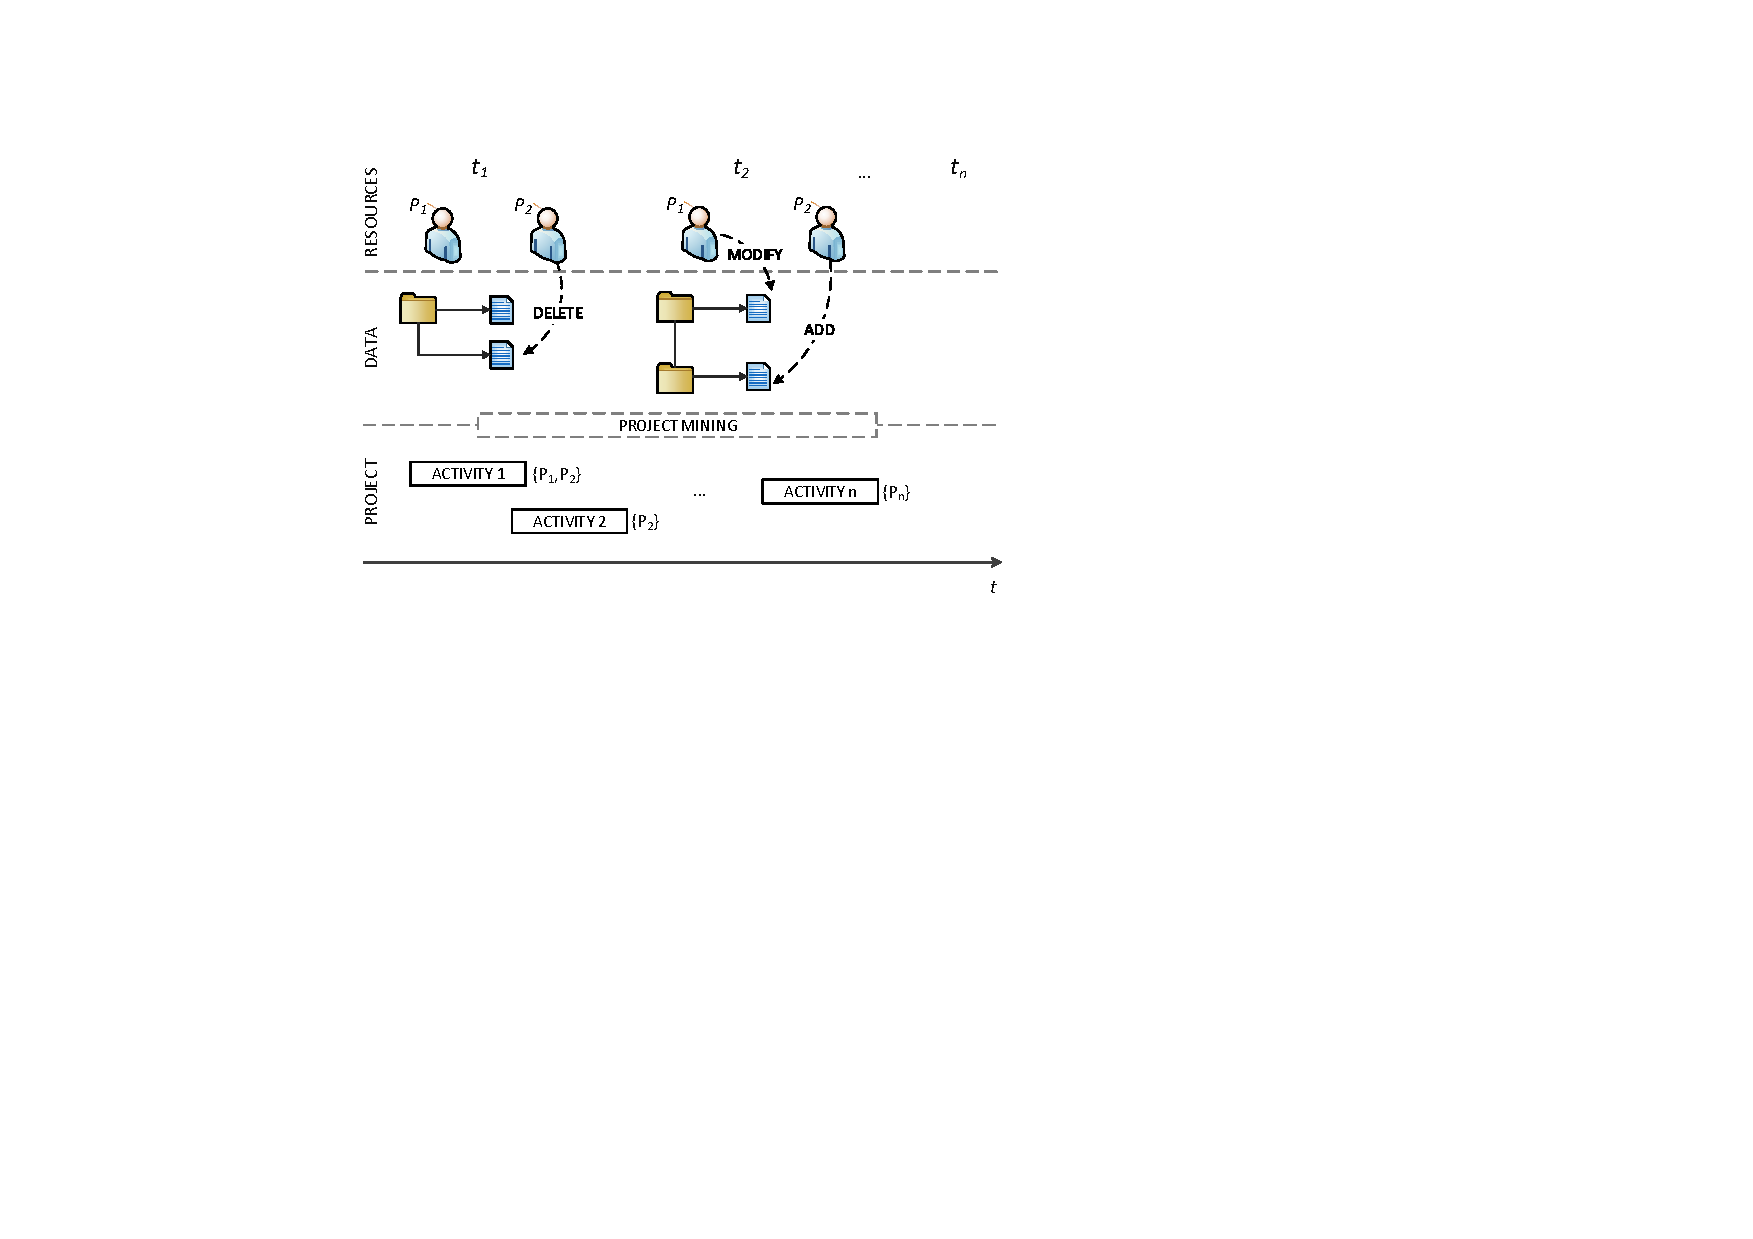
\includegraphics[width=.8\textwidth]{bpm2015/imgs/ProjectMining.pdf}
\caption{Problem illustration}
\label{fig:problem}
\end{figure}

Documentation is required not only explicitly as part of some activities but also to comply with norms and regulations that may require some evidence of the actions being performed in the organization. Documents are usually free of format or contain tables, at best. The unstructuredness of data makes it difficult to monitor processes and check rules on them. A starting point for analysis of project-oriented processes can be data logs %generated for  %usually consist of subversion projects
that are stored in Software Configuration Management (SCM) systems that help tracking the evolution of data and restore information if needed~\cite{voinea_open_2006}.
However, hundreds of versions of thousands of files are common in a single project~\cite{voinea_multiscale_2006}, which makes it impractical to browse this data manually.

%We focus on project mining motivated by a real case scenario in the scope of the SHAPE research project\footnote{\url{http://ai.wu.ac.at/shape-project/}}.
%The data log is provided by a Version Control Systems (VCS) whose information is not subdivided into traces related to process instances but consists of a hierarchy of work streams associated with individual files being added, modified or deleted in a subversion repository.

Let us see an example inspired by a real scenario of a process to write a project proposal that uses a Version Control System (VCS) to store the data. The project history, and hence, the data produced, starts when people begin to work on the proposal, which involves a description of the project goals and milestones, a division of tasks into work packages, an estimation of cost and resources required, etcetera. This information is spread in the repository over several folders containing different documents, which are later merged into a single file. If the proposal is accepted, the first step is to organize a kickoff meeting and assign specific resources to the work packages. A hierarchical set of folders is then created in the repository in order to store the information generated for each work package. As the project evolves over time, resources contribute by adding, removing or modifying information to the VCS repository. %\todo{Should answer point 3 on the review-list: Missing concrete examples of the need to “prove compliance to rules and regulations”. Which important rules and regulations will the analysis help comply with?} 
Project evolution is guided by specific norms that impose the execution of predefined steps. For instance, the European norm EN5016 requires a preliminary \gls{ram} analysis to support targets. 
%Data stored in the VCS can be used to prove compliance to rules and regulations of the domain. For instance, in the railway industry, 

Table~\ref{tab:example} depicts an excerpt of the log data generated, where the first column (on the left hand side) indicates the commit identifier, the second column indicates the person who committed changes, the third column indicates the commit date, %the fourth column shows (optional) descriptive information to clarify the scope of the changes performed
and the fourth column indicates the files affected and the type of action performed among added (A), modified (M) and deleted (D).
For the sake of simplicity, the table shows the log data of a specific time period and the actions related to a specific task, namely, $\defineExample$. That task was assigned to resource X % after a project meeting. %, when a part of project members asked for a toy example to better understand the problem domain.
and was supervised by resource Y and, later on, also by resource Z.
%An extract from the log concerning this period, that shows some crucial steps in the \emph{example} task, is reported on table \ref{tab:example}. Comments were left out from this representation, since at the current state we don't delve into them.

\begin{table}[bt]
\caption{Excerpt from VCS log data for the referenced time period }
\label{tab:example}
\scriptsize
{\renewcommand{\arraystretch}{1.3}
\centering
%\fontfamily{phv}\fontseries{mc}\selectfont
\begin{tabular}{m{.8cm} m{1.5cm} m{3cm} p{5.8cm}}
\hline\noalign{\smallskip}
%\hline
\textbf{CID}	 & \textbf{Resource} & \textbf{Date} & \textbf{List of changes} \\
%\noalign{\smallskip}
\hline
%\noalign{\smallskip}
\hline
\noalign{\smallskip}
\multirow{2}{*}{1} & \multirow{2}{*}{Y} & \multirow{2}{*}{2014-11-12~11:57:46} & A /example \\
& & & A \slash example\slash SHAPE\slash\-ToyStation\-Example.docx \\ \hline %\hdashline

%\multirow{2}{*}{205} & \multirow{2}{*}{X} & \multirow{2}{*}{2014-11-14 16:26:23} & A /example/ToyStation.bpmn \\
%& & & A /example/ToyStation.png \\ \hline %\hdashline

\ldots & \ldots & \ldots & \ldots \\ \hline

\noalign{\smallskip}
\multirow{2}{*}{3} & \multirow{2}{*}{X} & \multirow{2}{*}{2014-11-14 16:34:07} & M /example/ToyStation.bpmn\\
& & & M /example/ToyStation.png \\ \hline %\hdashline

%\multirow{7}{*}{207} & \multirow{7}{*}{X} & \multirow{7}{*}{2014-11-27 14:18:59} & M /example/SHAPE-ToyStation-Example.docx \\
%& & & D /example/ToyStation.bpmn \\
%& & & M /example/ToyStation.png \\
%& & & A /example/ToyStation\_0Loop.bpmn \\
%& & & A /example/ToyStation\_1Loop.bpmn \\
%& & & A /example/ToyStation\_nLoop.bpmn \\
%& & & A/example/ToyStation\_old.bpmn\\ \hline

%\ldots & \ldots & \ldots & \ldots \\ \hline

\noalign{\smallskip}
4 & W & 2014-12-15 13:49:11 & D /example/Download \\ \hline %\hdashline

\noalign{\smallskip}
5 & W & 2015-01-08 16:06:41 & A /example/Download2\\ \hline %\hdashline

\noalign{\smallskip}
\multirow{2}{*}{6} & \multirow{2}{*}{X} & \multirow{2}{*}{2015-01-13 11:47:09} & M /example/ToyStation\_0Loop.bpmn\\
& & & M /example/ToyStation\_nLoop.bpmn \\ \hline %\hdashline

\noalign{\smallskip}
\multirow{2}{*}{7} & \multirow{2}{*}{Z} & \multirow{2}{*}{2015-01-16 16:50:29} & A /example/ToyStation\_0Loop.pdf\\
& & & A /example/ToyStation-feedbackZ.pdf\\ \hline %\hdashline
\end{tabular}\\ \hfill
}
\end{table}

%Process mining techniques can help to discover processes from log data.
%Existing process mining techniques can deal very well with execution logs whose data is subdivided into \textit{traces} representing different process instances in which events are easily identifiable (e.g. through a \textit{caseId}).
%Procedural (e.g. BPMN~\cite{bpmn2_stable}, Petri nets~\cite{aalst_application_1998}, EPC~\cite{vanderaalst_formalization_1999}) as well as declarative (e.g. Declare~\cite{VanderAalst2009}, DPIL~\cite{zeising2014towards}) modeling languages can be used to represent the process discovered.
%Once a process model is discovered, it can be checked whether it is compliant with the existing (already known) process model and enhance the model or the way the process is executed accordingly.
%Performance can also be analyzed and compared to the expected values defined by key performance indicators (KPIs)~\cite{delrioortega_definition_2013}.

%\begin{table}[bt]
%\caption{Process mining vs. project mining}\label{tab:processVSprojectmining}
%\centering
%\begin{tabular}{l c c}
%%\hline\noalign{\smallskip}
%%\hline
% ~&~  Process Mining~&~Project Mining\\
%%\noalign{\smallskip}
%\hline
%%\noalign{\smallskip}
%Defined goals~&~  \cmark ~&~ \cmark \\
%Resource~&~ \cmark ~&~ \cmark \\
%Activities/Tasks~&~ \cmark ~&~ \cmark \\
%One time~&~ \xmark ~&~ \cmark \\
%Repetitive~&~ \cmark ~&~ \xmark \\
%\hline \\
%\end{tabular}
%\end{table}

%However, due to the ad-hoc nature of project-oriented business processes, the event logs for these processes look different.
%Therefore, mining of project-oriented business processes needs to be done in a different way.
%Whereas in traditional process mining the main goal is to discover the execution order and relation among activities, project mining aims at discovering the structure of the project along with its temporal progress and information about the actors involved.

% Deviations from the designed plan can then be measured, as well as the fulfillment of milestones, deadlines, resource usage constraints, cost expense, etcetera. Table~\ref{tab:processVSprojectmining} illustrates the main differences between process mining and project mining concepts\todo{CC: I'm not sure whether this table is representative and/or necessary}.


%\begin{table}[bt]
%\centering \begin{tabular}{m{1cm} m{2cm} m{2.8cm} m{3cm} l}
%%\hline\noalign{\smallskip
%\hline
%CID	&	Resource	&	Date	&	Message	&	List of changes \\
%%\noalign{\smallskip}
%\hline
%%\noalign{\smallskip}
%\hline
%\multirow{3}{*}{1} & \multirow{3}{*}{pol@uni.edu} & \multirow{3}{*}{2006-02-17 15:30} & \multirow{3}{*}{} & A /templates \\
%& & & & A /temp/costsplan.doc \\
%& & & & A /temp/proposal.pdf \\ \hline %\hdashline
%\multirow{3}{*}{2} & \multirow{3}{*}{al@co.com} & \multirow{3}{*}{2006-02-19 12:00} & \multirow{3}{*}{Reviewed proposal} & A /slides \\
%& & & & A /slides/review.doc \\
%& & & & M /temp/proposal.pdf \\ \hline %\hdashline
%\multirow{2}{*}{3} & \multirow{2}{*}{al@co.com} & \multirow{2}{*}{2006-02-19 17:05} & \multirow{2}{*}{Renamed a file} & D /temp/proposal.pdf \\
%& & & & A /temp/proposal\_final.pdf \\ \hline %\hdashline
%\multirow{2}{*}{4} & \multirow{2}{*}{jb@uni.edu} & \multirow{2}{*}{2006-02-23 11:05} & \multirow{2}{*}{Added CV} & \multirow{2}{*}{A /skills/CV.pdf} \\
%& & & & \\ \hline %\hdashline
%\multirow{2}{*}{5} & \multirow{2}{*}{ccm@uni.edu} & \multirow{2}{*}{2006-02-19 17:05} & \multirow{2}{*}{WPs description} & A /goals/WPS\_description.doc \\
%& & & & M /temp/costsplan.doc \\ \hline %\hdashline
%\multirow{2}{*}{\ldots} & \multirow{2}{*}{\ldots} & \multirow{2}{*}{\ldots} & \multirow{2}{*}{\ldots} & \multirow{2}{*}{\ldots} \\
%& & & & \\ \hline
%\end{tabular}\\ \hfill
%\caption{A representation of VCS log data}
%\label{tab:VCSlog}
%\end{table}

%\begin{figure}
%\centering
%\includegraphics[height=6.2cm]{imgs/pm-pic}
%\caption{Problem illustration,}
%\label{fig:example}
%\end{figure}

Existing frameworks, such as Subversion or Git, allow to access their logs in different ways. However, the covered information is limited to (roughly) that depicted in Table~\ref{tab:example}. Especially for big projects that are frequently updated over a large period of time, these logs are complex to analyze.
Therefore, the problem to address is how to analyze and visualize the information produced in project-oriented business processes such that it can be represented in an understandable and manageable way by project experts and
enable, a.o., the automation of mechanisms for compliance checking.
The following properties of project-oriented process logs must be taken into account to achieve this goal: (i) VCS repositories consist of a hierarchy of folders and files which are logically organized such that work is grouped in a specific way; (ii) process activities are not registered in VCS log entries. Therefore, such information must be inferred by reasoning on the repository structure and/or the content of the log entries; (iii) the granularity of the events is unknown a priori and it needs to be defined before analyzing the data.
%Therefore, the goal of project mining is to represent that data in a way that is natural to the project (i.e., by deriving the project structure and its progress over time) taking into consideration the aforementioned properties of VCS logs.

%\begin{itemize}
%\item we cannot see activities, but we can see that work was done
%\item hierarchical work structure (requirements)
%\item names of activities are not directly explicit
%\item granularity of events (e.g. in our case is on the file level)
%\end{itemize}

%We need to retrospect that the things that we did in the project were complete and correct. Answer to questions like: Did we do all the stuff?\\ \hfill

%Logs carry much more information (such as the number of lines or bytes modified in a file) but for the moment let's treat only this level of granularity.

%\todo[inline]{CC: Some further work is required on sections 2.1 and 2.2 so that the transition from the former to the latter is smooth and the last part of section 2.2 makes sense}


\subsection{Related Work}\label{sec:bpm2015:related}

The problem described has been addressed in the literature from different perspectives. The first category of related work tackles the problem by transforming it into a process mining problem. Consequently, approaches have been developed to preprocess VCS data such that process mining techniques can be applied, and hence, a business process can be derived from the log data.
In this group, Kindler et al. \cite{kindler2006activity,kindler2006incremental} developed an algorithm for extracting software processes that are mapped to Petri Nets. Activities, which are not explicit in the logs, are discovered from their input and output artifacts. However, strong assumptions are made on the filenames as well as on the software process lifecycle. %(always design, code, review, testres). Activities (which are not explicit in the logs, like in our case) are discovered from their input and output artifacts. Here defined as triples $<I,O,R>$ where I=input, O=Output, R=resouce who perfomed it.
Rubin et al. in \cite{rubin2007process} addressed the problem of engineering processes that are not well documented and are usually unstructured. They provided a bridge from Kindler et al.'s approach to ProM \cite{van2005prom} in order to mine different process perspectives, such as performance social network analyses. %but not from a project point of view.
Rubin et al. \cite{rubin2014agile} applied process mining to the touristic industry and obtained user processes from web client logs pursuing the goal of improving the software system by analyzing the underlying process.
Poncin et al. \cite{poncin2011process} developed the FRASR framework for preprocessing software repositories to transform the VCS data to logs that conform to the process mining event log meta model~\cite{van2005meta} as utilized in ProM \cite{van2005prom}.
However, these approaches disregard the single-instance nature of project-oriented business processes and treat them as procedures that can be repeated over time.

The second category of related work focuses on the visualization of VCS data %by defining measurements such as things that can be plotted into a chart.
for different purposes.
%There are two main lines of how this problem was approached in literature.
%\paragraph*{visualization perspective} defining measurements such as things that can be plotted into a chart. But, they haven't any explicit notion of work structure.
%\paragraph*{preprocessing} - VCS data is transformed in order to comply to the process mining meta model from van Dongen and van der Aalst \cite{van2005meta}. This means that they are oriented to discover "classical" processing (i.e. repeated many times in the logs).
Several approaches study the interaction among developers over time from a visualization point of view. For instance, Ogawa and Ma \cite{ogawa2010software} drew storyline pathways to show the story of each developer's contribution. Other approaches analyze and visualize VCS data at file level in order to discover file version evolution. Voinea and Telea~\cite{voinea_multiscale_2006} introduced an interactive navigation method to surf file version evolution as well as two methods to cluster versions of the same file in an abstraction layer. Wu et al.~\cite{jingwei_evolution_2004} also visualized the evolutions of entire projects at file level, emphasizing the evolution moments.
Finally, several approaches study change prediction with the aim of discovering prediction patterns that can help in the process of software development~\cite{zimmermann_mining_2004,ying_predicting_2004}.
%Feld et al. \cite{feldt2013supporting} used software project data to \emph{predict} potential problems during development. Heatmaps, used to visualize source code changes in a two dimensional space, showed to be easily readable also by non experts.
The approaches mentioned in this category as well as others that apply similar techniques~\cite{feldt2013supporting,kagdi_mining_2006,dambros_flexible_2008} focus on studying software evolution from different standpoints. However, the goal pursued differs in all cases from our goal in that they are not interested in discovering projects tasks out of the log data, and hence, they lack an explicit notion of work structure that we need to consider for our purpose.

Our approach combines ideas from both areas, as we aim at identifying tasks like in the approaches that rely on process mining, but we must cluster the data in an appropriate way, for which techniques developed in the approaches that pursue visualization may be adapted or extended.

%----------------
%
%Then explain that, in our work, we don't only want to see what's happening. We want also compliance (which means: did things happen in the right way (as they were allowed to)? Compliance can be provided by Process Mining algorithms... but we cannot apply process mining techniques directly (because they need logs structured in different ways - not svn/git logs). Thus, we need to adopt this strategy. 
\section{Mining VCS Event Data}
\label{sec:bpm2015:concept}
Here, we first formalize the notions encountered in the project mining setting. Then we develop an approach to acquire a hierarchical overview on the project from a repository perspective.

\subsection{Preliminaries}
\Glsfirst{vcs} are used in projects to ensure reliable collaboration. We build our approach on \gls{vcs}. Typically, the workflow in \gls{vcs} is that people work on files (e.g., text, source code, spread sheets) and commit them to the central repository. Project participants comment on their commits so that other participants can better understand the nature of the changes to the files.

Let \Files be the universe of files. Files are organized in a file tree. Therefore, each file $\file \in \Files$ has one parent file. The only file without a parent file is the root file. We capture this information in the parent relation $\parent : \Files \times \Files$. For example, let $\file_p \in \Files$ be the parent of file $\file_c \in \Files$, then $(\file_p, \file_c) \in \parent$.
The transitive closure on the parent files is given by the function $\ancestor : \Files \rightarrow 2^{\Files}$ that returns the set of files along the path to the root.

When project members did a certain amount of work and want to save their current progress, they commit the changes to the \gls{vcs}.
We define changes on files as the events of interest on the lowest granularity.
\begin{definition}[Event] \label{def:events}
Let $\Events$ %  = \Files \times \ChangeOperations \times \Timestamps \times \Comments \times \ChangedAmount$
be the set of events. An event $\event \in \Events$ is a four-tuple $(\file, \changeOperation, \timestamp, \comment)$, where
\begin{compactitem}
  \item $\file \in \Files$ is the affected file of the event.
  \item $\changeOperation \in \ChangeOperations =\lbrace\added$, $\modified$, $\deleted \rbrace$ is the change operation on the file with obvious meaning.
  \item $\timestamp \in \Timestamps = \mathbb{N}_0$ represents a unix time stamp marking the time of the event occurrence.
  \item $\comment \in \Sigma^*$ is a comment in natural language text.
%  \item $\changedAmount \in \ChangedAmount$ is the absolute number of changed bytes in comparison to the previous version of the file.
\end{compactitem}
% Let $\ChangeOperations = \lbrace \added$, $\modified$, $\deleted \rbrace$ be the set of change operations on files, \Timestamps represent unix time stamps, and $\Comments \subseteq \Sigma^*$ be comments in natural language text.
% Events $\event \in \Events$ are tuples of the form .
% \todo{TODO: decide, if we need weights on how much of the files changed.
% Also: what about resources?}
%$\file \in \Files$ is a file, $\changeOperation \in \ChangeOperations$ is a change operation, $\timestamp \in \Timestamps$ is a timestamp, and $\comment \subset \Sigma^*$ is a comment in natural language text.
\end{definition}

For events $\event = (\file, \changeOperation, \timestamp, \comment%, \changedAmount
)$ we overload $\file, \changeOperation, \timestamp$, and $\comment$
%,$ and $\changedAmount$ 
to be used as accessor functions. For example, \file is the function $\file : \Events \rightarrow \Files$ mapping an event to its affected file.

Project participants can commit a number of changes to different files at one step. Therefore, we define the notion of commits as follows.
%\todo{Maybe instead use a reduction of an event like $\event_{|\timestamp}$}

\begin{definition}[Commit]
A commit $\commit$ is a set of events sharing the same time stamp and comment, i.e., $\forall \event, \event' \in \commit: \timestamp(\event) = \timestamp(\event') \wedge \comment(\event) = \comment(\event')$. Additionally, each event in a commit affects different files, i.e., $\forall \event, \event' \in \commit : \event \neq \event' \rightarrow \file(\event) \neq \file(\event')$.
\end{definition}
%\todo{Decide: Do we need the definition Commits at all?}

Usually, it is in the hands of project participants, when they decide to commit changes to the \gls{vcs}. In the extreme case, there could be only a single commit made in a project that adds all files to the repository.
Note that this extreme practice would render the use of a \gls{vcs} obsolete. On the contrary, it is common practice to regularly perform commits in order to securely store work progress and to reduce the chance of conflicts~\cite{pilato2008version,DBLP:conf/seke/HouMCX14}. Conflicts occur, when another participant committed changes to a file that is being committed and can cause extra work.
Based on these insights, we make the assumption that commits are regularly made during work.

Projects are decomposed into work packages. We assume a hierarchical work package structure of a project, such that a work package can have sub work packages. Further, the amount of work in a single work package need not be done in one single time span, but it can be split into several activities. Activities have a start and end time, and subsequent activities can have idle periods in between. Thus, we define projects as follows.
\begin{definition}[Project]\label{def:project}
A project \Project is a tuple $(\WorkPackages, \Structure, \Activities, \startTimeFunction, \finishTimeFunction, \MappingFunction)$, where
\begin{compactitem}
  \item $\WorkPackages$ is the set of work packages in the project.
  \item $\Structure \subseteq \WorkPackages \times \WorkPackages$ is the relation that hierarchically decomposes work packages into a tree structure.
  \item $\Activities$ is the set of activities that are conducted in the work packages.
  \item $\startTimeFunction : \Activities \rightarrow \Timestamps$ is the function that assigns a start time to activities. Activities are ordered by their start times.
  \item $\finishTimeFunction : \Activities \rightarrow \Timestamps$ is the function that assigns an end time to activities.
  \item $\MappingFunction : \Activities \rightarrow \WorkPackages$ is the mapping function that maps activities to their corresponding work packages.
\end{compactitem}
\end{definition}

Note that this definition reflects an activity centric view on projects. The definition deliberately omits further dimensions, e.g., costs, resources, risks. The idea is not to capture projects in every detail, but to focus on the work packages of a project to obtain an overview of the work that is being done. %\todo{Question: do we want a full-blown definition on projects? with risks, resources, milestones, stakeholders, \ldots?}
We are interested in when work has been started in a work package, and when work packages have been done. This information can be derived from the activities associated to the workpackages. An obvious assumption is that the work package starts with its first activity, and ends when its last activity is completed.

Based on these notions, we can define the task of \emph{project discovery} as reconstructing the project \Project from a set of low level event data \Events.
In the following, we present an approach to this problem.

% \begin{definition}[Project mining]
% 	Given a set of events \Events, the objective of project mining is to identify:
% 	\begin{compactitem}
% 		\item the set of work packages \WorkPackages in the project.
% 		\item the start \startTimeFunction, and end \finishTimeFunction of the workpackages in \WorkPackages.
% 		\item the hierarchical relation \Structure between work packages.
% 		\item the mapping function \MappingFunction that assigns assigns events to a work package.
% 	\end{compactitem}
% \end{definition}


% Inital definition which we have to align to the current \\
% A commit is a set of change operations. $\commit \equiv \lbrace c \in \changeOperation \rbrace \times \comment$ \\
% A change operation is a set of triples $\changeOperation \equiv \lbrace F, W, O \rbrace $ where $F, W, O$ are respectively the file, the weight (how much a change affected the file), and the operation type ($O={modified,added,deleted}$)\\
% Upon the above sets we can define functions such as a modification function (that, for instance, maps the set of files to their weight), or distance(f1, f2) (but for the moment we don't use it).\\ \vfill

% After the last discussion I identified the following concepts to be formalized. So basically we would need to align the initial definition to was follows.
%
% Definitions: \\
% \begin{definition}[Event]
% Event: something that happens at some point in time. Generally in the past. (Primitive concept: can't be derived from any other concepts? Can it be defined?!)
% Event data: data regarding events. An event over a dataset A is the minimum amount of modification made to the minimum part of A at some point in time. i.e. the smallest possible change.
% \end{definition}
%
% \begin{definition}[Project]
% D2. Project (hierarchy) \\
% a project has a hierarchy. It is a set of event streams. An event stream is an object of the hierarchical structure. (that relates to events).
% \end{definition}
%
% We define a mapping function $f$ from the set of events to objects which is:
% \begin{itemize}
% \item surjective and not injective (i.e. every element in the codomain has a corresponding element if the domain, and it doesn't hold that for two different elements $a, b$ of the domain there exist two different mappings $f(a), f(b)$ in the codomain.
% \item total
% \end{itemize}
%
% Function $f$ partitions the set of events...
% \begin{definition}[Commit]
% A commit is a "bundle" of events.\\
% \end{definition}

% \begin{definition}[Drill]
% Here we formally define the agglomeration feature. We can drill-up and drill-down on the data. E.g. show grouped events for folders at different levels.
% \end{definition}

\subsection{Project Discovery Technique}\label{sec:bpm2015:subsec:bpm2015:discovery_technique}
\begin{figure}[b]
\centering
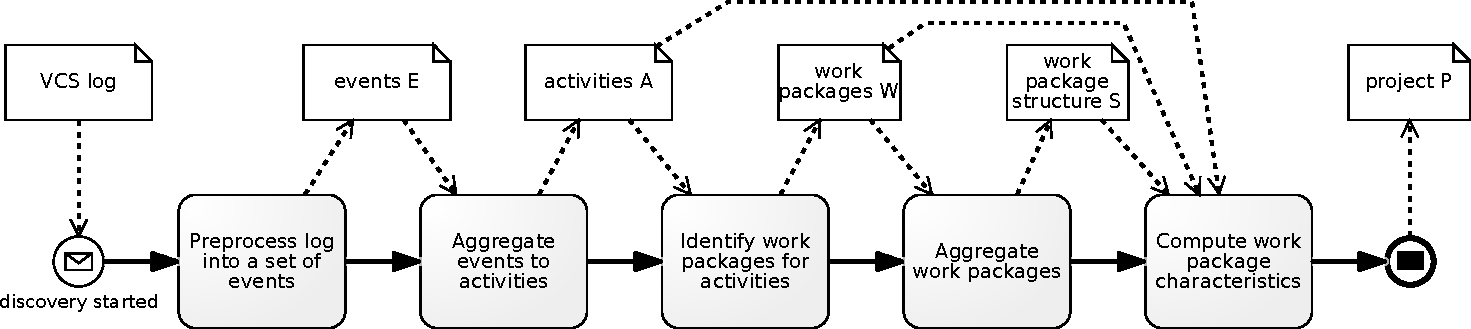
\includegraphics[width=\textwidth]{bpm2015/imgs/Project_discovery}
\caption{Project discovery technique overview as BPMN process model.}
\label{fig:bpm2015:project_discovery_technique}
\end{figure}
For project discovery from the \gls{vcs} commit history, we need to identify activities that are performed, associate the activities to work packages and recreate the work package structure of the project.
Our aim is to create a hierarchical model that provides an overview of the project work.
Therefore, we have to identify the start and end times of activities and of work packages before we can visualize the project work. The input to the technique is the log that is stored in the \gls{vcs}. The challenge is that the raw log only records commits on the file system level and information on activity level is missing. However, we can deduce activity information from events based on the following assumptions.

\begin{description}
  \item[A1: Meaningful file tree structure.] The file tree structure in a project represents its work package structure. That is, the knowledge workers organize their work in a file hierarchy that reflects the project structure.
  \item[A2: Local changes.] Activities in a work package affect only files of the work package folder, or in the corresponding sub-tree in the file tree structure.
  \item[A3: Frequent commits.] Commits to the \gls{vcs} are regularly performed, when conducting work in an activity.
\end{description}

Note that assumption A1 can be seen as a strong assumption on the file tree structure. Nevertheless, we argue that even if A1 is not entirely met, the aggregation of work information on the file tree hierarchy provides a valuable view on the project.
Figure~\ref{fig:bpm2015:project_discovery_technique} shows the different steps of the technique. We describe each of them in detail.

\subsubsection{Step 1: Preprocessing.} The first step is to transform raw logs of version control systems (which might be grouped by commits) into a list of events as specified in Definition~\ref{def:events}. This step is easily done by replicating the information on commit level to be contained in the events. The output is a set of events \Events.

\subsubsection{Step 2: Aggregating events to activities.}
Given the set of events \Events that we gathered from a version control system, the next step is to identify the activities to which the events belong. Note that we do not know the activities of the project in advance, but need to infer them based on the events. Each event affects a single file in the file hierarchy.

\begin{figure}
\centering
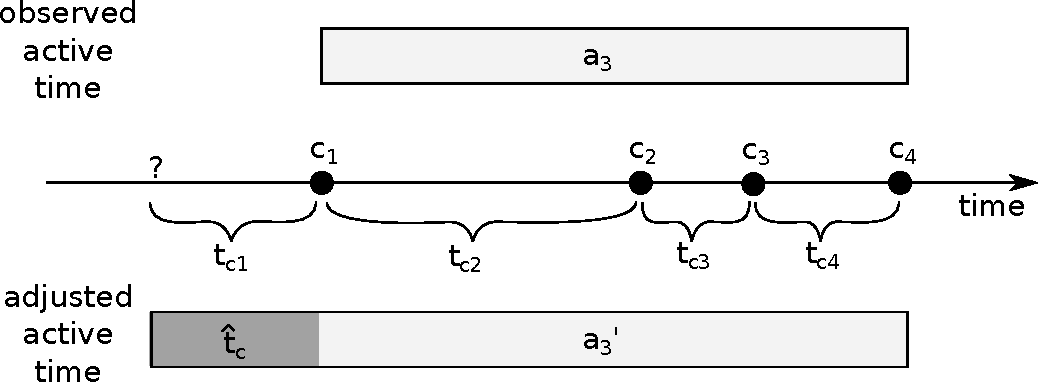
\includegraphics[width=.7\textwidth]{bpm2015/imgs/activity_adjustment.pdf}
\caption{Adjustment of activity start time \startTimeFunction. }
\label{fig:bpm2015:activity_adjustment}
\end{figure}

Based on assumption A2, we are interested in activities conducted in a work package, that is, we filter for the events that are contained in the given file or its children. For every file $\file$ of interest, we select the set of events affecting the file or its children as $\Events_{\file} = \lbrace \event \in \Events \mid \file = \file(\event) \vee \file \in \ancestor(\file(\event))  \rbrace$. The task is then to find the activities which emitted the set of events $\Events_{\file}$. We rely on assumption A3, which states that during an activity, we expect multiple commits. Assumption A3 allows us to conclude that if we do not observe commits for a longer period of time, there is no activity being performed in the work package.

%To derive coarse grained activities from low level events, clustering techniques~\cite{Berkhin2006ClusteringSurvey}, or abstraction functions~\cite{baier2014bridging} can be used.
%Former assume that a distance function measures the distance between events, and partitions the set of events into groups. Well-known examples are the k-means clustering~\cite{Berkhin2006ClusteringSurvey}, or hierarchical agglomerative clustering.
To this end, we adopt the abstraction technique by Baier et al.~\cite{baier2014bridging} and allow the domain expert to formulate rules for aggregating events to activities based on boundary conditions. Assuming that people frequently commit their progress (A3), we can specify a boundary condition based on the temporal distance to previous events. For example, we can specify that a time period of seven days without a commit is a boundary condition. %But also other boundary conditions can be selected, e.g., based on resources.
As the result, we obtain the mapping from events to these activities, which we call $\eventMapping_{\file} : \Events_{\file} \rightarrow \Activities_{\file}$ in the remainder of the paper. The set of discovered activities identified for the work package based on given boundary conditions is then $\Activities_{\file} = \lbrace \activity \mid \event \in \Events_{\file}, \eventMapping_{\file}(\event) = \activity \rbrace$. We also define the inverse mapping, that is, the mapping from an activity to its events as $\eventMapping_{\file}^{-1} : \Activities_{\file} \rightarrow 2^{\Events_{\file}}$.

With the events mapped to activities, we need to find the temporal boundaries of the target activities. That is, we define the functions $\startTimeFunction$ and $\finishTimeFunction$ for each activity. The challenge here is that we do not know when an activity actually started, because the start of the activity is not recorded in the \gls{vcs}. We can only observe the time of the first commit in that activity, but commits usually mark progress of an already running activity.

To address the challenge of missing start times, we impute the missing start time by prepending the expected active time $\expectedActiveTime$ before a commit, as illustrated by Figure~\ref{fig:bpm2015:activity_adjustment}. This notion assumes that project participants commit their work progress after a certain amount of time. However, we cannot compute \expectedActiveTime by looking at the average commit rate in a work package, because this average is based on busy periods and idle periods. We need to factor out the idle periods in the computation of this measure.
%Therefore, we use the following formula.
%Let $\file$ be a file in the file tree that represents a work package, and let $\Events_{\file}$ be the corresponding events for all the children of $\file$. Let further $\Activities$ be the activities identified for the work package based on given boundary conditions.
We know the end time of the activities, as the last commit marks the completion of work. Therefore, each activity \activity based on given boundary conditions has the associated end time $\finishTimeFunction(\activity) = \max(\lbrace \timestamp(\event) \mid \event \in \eventMapping_{\file}^{-1}(\activity)  \rbrace)$. Further, we write the first event's timestamp of an activity as the function $\startTimeFunction'(\activity) = \min(\lbrace \timestamp(\event) \mid \event \in \eventMapping_{\file}^{-1}(\activity)  \rbrace)$.
Then, we define $\numCommits:\Activities_{\file} \rightarrow \naturalNumbers$ as the number of commits in one activity, formally $\numCommits(a)=|\lbrace \commit \mid \event \in \commit \wedge \eventMapping_{\file}(\event)=a\rbrace |$.

With this information the expected active time between commits \expectedActiveTime is given as follows.

\begin{equation}
	\expectedActiveTime = \frac{\sum_{\activity \in \Activities_{\file}} \left(\finishTimeFunction(a) - \startTimeFunction'(a)\right)}{\sum_{\activity \in \Activities_{\file}} (\numCommits(\activity)-1) }
\end{equation}

We assume that there is at least one activity spanning over at least two commits, i.e., $\exists \activity \in \Activities_{\file} \mid \numCommits(\activity) > 1 $. Translated to our boundary condition, this assumption is that there is at least one week in each work package, in which there were at least two commits made. Otherwise, we set $\expectedActiveTime$ to 0 for the current file \file due to lack of information.

Given the expected active time between commits $\expectedActiveTime$, we can finally adjust the start time of each activity. Therefore, we set the associated start time for each activity as $\startTimeFunction(\activity) = \startTimeFunction'(\activity) - \expectedActiveTime$. That is, we subtract the expected active time from the first commit's timestamp.

We apply Step 2 to all files $\file$ in the file tree to get $\Activities_\file$. For the remainder of this paper, we define the function $\fileToActivity : \Activities \rightarrow \Files$ that contains the mapping information of the discovered activities to their originating files. Finally, we set the activities \Activities in the project to be the union of the activity sets per file $\bigcup_{\file \in \Files} \Activities_\file$.

% \begin{definition}[Abstraction Function]
% Formally, we rely on an abstraction function $\abstractionFunction : 2^{\Events} \rightarrow 2^\Activities$ that maps a set of events to a set of activities.
% \end{definition}
%
% The abstraction function \abstractionFunction operates on a set of events


\subsubsection{Steps 3 and 4: Mapping activities to work packages and aggregating.}
Once activities have been identified, we want to climb to the next abstraction layer: the work packages. Assumption A1 allows us to specify a one-to-one mapping $\kappa : \Files \rightarrow \WorkPackages$ between files in the file tree structure and work packages. More precisely, we construct the set of work packages $\WorkPackages$ isomorphic to the set of files $\Files$, such that the $\parent$ relation is preserved in the work package structure \Structure relationship. %This way, we assign the discovered activities of a selected file $\file'$ to the work package corresponding to $\file'$.

The mapping $\MappingFunction$ of activities to work packages is simply $\MappingFunction(\activity) = \kappa (\fileToActivity(\activity))$. That is, the corresponding work package of the activity that was discovered for a file.
%The aggregation of work packages is done according to the hierarchy obtained from the file tree structure.
In this way, we provide an activity based view on work packages, and we can aggregate on each level in the file system to see active periods of the corresponding hierarchy level.


\subsubsection{Step 5: Computing work package characteristics.} In this final step, we compute measures of interest for the discovered work packages. First, we obtain the temporal boundaries of a work package by the functions $\startTimeFunction$ and $\finishTimeFunction$ of the associated activities.

Let $\MappingFunction^{-1} : \WorkPackages \rightarrow 2^{\Activities}$ be the inverse of the mapping function $\MappingFunction$ of the project.
The start and end time of a work package ($\startTimeFunction_{\WorkPackages}$ and $\finishTimeFunction_{\WorkPackages}$) are functions from work packages to timestamps. The start time is defined as $\startTimeFunction_{\WorkPackages}(\workPackage) = \min(\lbrace \startTimeFunction(\activity) \mid \activity \in \MappingFunction^{-1}(\workPackage)\rbrace )$, and the end time function of work packages $\finishTimeFunction_{\WorkPackages}$ is analogously defined using the maximum of the end times $\finishTimeFunction(\activity)$ of the activities.
We call the duration of a work package $\durationOfWorkPackage$ that is the difference between $\finishTimeFunction_{\WorkPackages}$ and $\startTimeFunction_{\WorkPackages}$.

Moreover, we are interested in the ratio of active working periods (i.e., the time spans of activities) to the total work package duration. This quantity helps to estimate the average work intensity in a work package.

\begin{definition}[Coverage]
The coverage \coverage of work packages by activities is a function $\coverage : \WorkPackages \rightarrow [0,1]$ and is defined as follows.
\begin{equation}
\coverage(\workPackage) = \frac{\sum_{\activity \in \MappingFunction^{-1}(\workPackage)}  \left(\finishTimeFunction(a) - \startTimeFunction(a)\right)}{\durationOfWorkPackage(\workPackage)}
\end{equation}

\end{definition}

With this final step, we lifted the information hidden in low level events to a high-level Gantt chart perspective, with which project managers are familiar. In the following, we compare our technique to existing process mining approaches.


% Here, we present a first approach to project mining that serves to offer a rough estimation on the work packages and their structure in a project.
% The proposed approach in this paper builds on the assumption that the file structure in the project repository is meaningful.
%
% %We acknowledge that this assumption might not be valid in all cases, but we shall demonstrate the usefulness of the approach
%
% Based on this assumption, the main task of project mining is to identify activities that are performed and map them to the work packages of the project.
%
%
%
% The approach is based on the general assumption that there is a \emph{distance} between events and we can algorithmically measure it.



% Technique: \\
%
% Algorithm (from VCS to project) \\
% \begin{verbatim}
% pseudocode of the algorithm
% \end{verbatim} 
\section{Evaluation}\label{sec:bpm15:evaluation}

In this section we evaluate our solution to the project mining problem, and show results for the example presented in Section~\ref{sec:background}.

\subsection{Experimental setup}

%
%This section should clarify the objective of the evaluation. What do we try to study with the evaluation (which quality characteristics)? This also relates to the question whether we let the result speak for itself or if we benchmark with competing approaches. here, you should also mention that the technique was implemented as a prototype.

We evaluate our technique by a visual perspective and by comparison to possible different approaches. To this end we implemented our technique as a prototype. We used JAVA as a programming language to code the logic of our technique. For the visualization part we made use of custom SWT widgets provided by the Nebula Project\footnote{https://www.eclipse.org/nebula/}. Our program can deal with logs from Subversion (SVN) \citep{pilato2008version} and Git \citep{torvalds2010git}, but it can be extended to other version control systems by providing an implementation of the preprocessing step discussed in Section~\ref{sec:bpm2015:subsec:bpm2015:discovery_technique}.
We ran the software in an Intel\textregistered Core \texttrademark~i5-4570 CPU @ 3.20 GHz x 4 machine with 15.6 GiB of RAM and Linux kernel 3.13.0-46-generic 64-bit version.

\subsection{Input data description}

We tested our prototype with real-world log data taken from the SHAPE project. Logs were exported from the SVN and Git repositories of different projects. They come from the railway domain and describe engineering processes. Documentation stored in the repositories consists of manually produced text files, diagrams, and files coming from proprietary tools that are typically used in the domain.

We will display results for the SVN log that describes the process oriented project for SHAPE. Data span over one year, going from January 2014 to January 2015. This time window covers the phases of project definition and planning, and a part of the project execution. In the first phase, feasibility of the project was studied and budget, schedule and resources were determined. Proposal submission marked the end of this phase. The second phase started with a kickoff meeting in October 2014 and is still ongoing.

The total number of participants who actively contributed to the work packages stored in the SVN repository was 8 people in the beginning, with new resources joining the project after the kickoff date. The total number of files and directories counts up to 156 objects and 226 overall commit events. The total number of extracted change events after preprocessing (i.e. atomic changes on all the files) was 453.

The last part of the log data contains the task \defineExample, introduced in Section~\ref{sec:problem}. For our showcase we assume that this task is contained in a work package named \emph{example}.

\subsection{Output data}

To monitor the project execution, we visualize the work progress that was done for each work package. Monitoring is performed by managers who want to have an overview on the project (which work packages are done, when and for how long, and where idleness or congestion occurs). Gantt charts offer a graphical representation for displaying schedules and jobs that were done on the various work packages \citep{wilson2003gantt} in a way that can easily be communicated to managers.

\begin{figure}
\centering
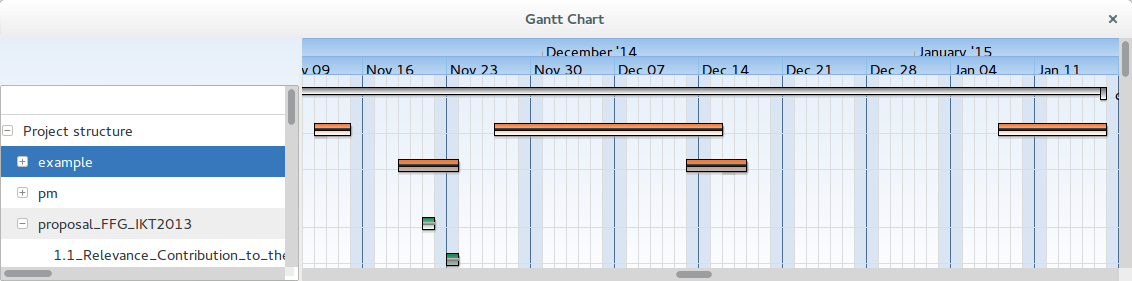
\includegraphics[width=\textwidth]{bpm2015/imgs/aggregation_and_not}
\caption{Data representation from our tool. Atomic events are drawn as dot with a minimal duration and different color per commit. }
\label{fig:example-screenshot}
\end{figure}

Figure~\ref{fig:example-screenshot} is a screenshot of how our tool presents the data. The tree structure on the left represents the \parent relation in the file tree. Events belonging to the same commit have the same color. On the top part of the chart we can see the result of merging events to activities with our aggregation method. Here we have merged the events of the example scenario on their highest abstraction level. The chart shows the three main activities and the idle times between them. %It is possible now to have an overview of the three main active periods in the work package.
On the other hand, in correspondence to expanded directories we show only their status before the aggregation. That is, every time a directory is fully expanded we apply a disaggregation into the corresponding activities. In this way, we can also show the finest granularity of work, i.e. the atomic events.

\subsection{Project Analysis}
Next, we apply our algorithm to the example case from Table~\ref{tab:example} and check how it helps to identify work packages. The data is aggregated according to our threshold of seven days. We can observe three groups of events being temporally close to each other according to our threshold. That is, we expect the event data to be grouped into three activities.

The second step of our algorithm takes care of adjusting the starting time of the activities. Furthermore, we vertically order the events and activities in the Gantt chart according to the directory structure to show the mapping from the objects on the Gantt chart to each work package in the tree structure. The last step, computing work package characteristics is done automatically when we collapse a node on of tree.

\begin{figure}
\centering
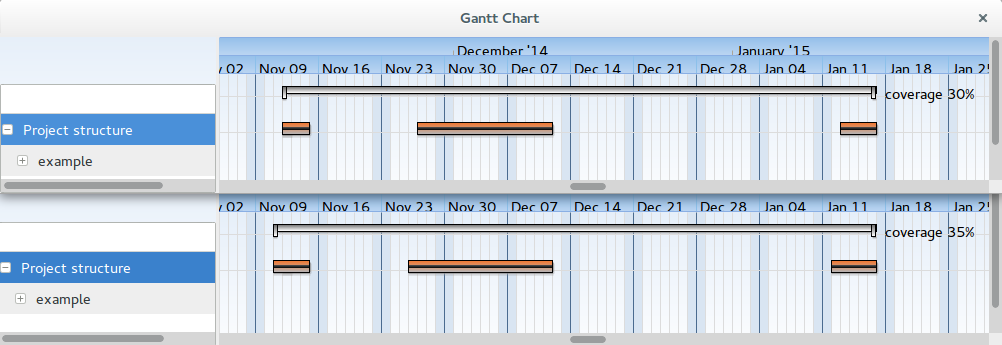
\includegraphics[width=\textwidth]{bpm2015/imgs/coverage_before_and_after}
\caption{Before and after the prepending the expected time before commit. Coverage factor increases when we adjust the starting times of the activities.}
\label{fig:example-collapsed}
\end{figure}

Figure~\ref{fig:example-collapsed} shows a comparison of the case when we do not implement the activity adjustment to the case which adjusts it. In the upper part, activity boundaries are based only on the first commit time that we see in the data. In the lower part, we observe that the start times were adjusted by approximately one day. The tool automatically adjusted the start time of the activities. As a consequence, the coverage factor increases because we expect that there was more work than what we observe by only considering the first commit time.

\subsection{Coverage tests on available open projects}

Finally, we apply our approach on different input data from open source projects. We are interested in exploring how the coverage factor varies in different existing projects. Hence, we take the work package $\workPackage$ as our controlled variable and set it to the highest level of aggregation. Then, we analyze each project of the data set and observe the dependent variable $\coverage(\workPackage)$.
Another variable of interest is the $\expectedActiveTime$ since it gives an idea of the average work speed (commit frequency) during active times.

\begin{table}
\caption{Coverage results for different open source projects}
\label{tab:experiments}
\centering
\begin{tabular}{rcccccc}
\hline\noalign{\smallskip}
\textbf{Log} ~&~ \textbf{Duration} ~&~ \textbf{Idle periods} ~&~ \textbf{Files} ~&~	 \textbf{Commits} ~&~	\textbf{$\expectedActiveTime$} ~&~ \textbf{$\coverage(\workPackage)$}\\
File name ~&~ Days ~&~ Number ~&~ Number ~&~ Number ~&~ Hours ~&~ \% \\
\hline \hline
\noalign{\medskip}
MiningCVS &	24 & 0 & 89  &	 63 & 9 & 100 \\
%\hline

Whitehall & 1279 & 6 & 6539  &	15566 & 2 & 95 \\
%\hline

Petitions &	834 & 17 & 1562  &	914 & 13 & 59 \\
%\hline

Study &	624 & 13 & 7501  &	736 & 11 & 58 \\
%\hline

The Guardian &	1667 & 59 & 12889  &	 621 & 30 & 44 \\
%\hline

Book &	414 & 15 & 154  & 592 & 5 & 32 \\
%\hline

Papers &	 1859 & 55 & 1791  &	 649 & 20 & 30 \\
%\hline

Requirements & 771 & 22 & 505  &	231 & 17 & 21 \\
%\hline

Yelp &	206 & 6 & 24  &	54 & 20 & 20 \\
%\hline

Adobe &	1076 & 13 & 356  &	237 & 24 & 15 \\
%\hline

\hline
\end{tabular}%\\ \hfill
\end{table}

%We test our tool on log data from open source projects that we find available on the web and data from SHAPE.
The data we used stems from the following projects. \emph{MiningVCS} is our tool. It consists of daily commits and was developed over 24 days.
\emph{Whitehall} is the code name for the Inside Government project, which aims to bring Government departments online in a consistent and user-friendly manner. \emph{Petitions} is a Drupal 7 code base used to build an application on "We The People", the platform to create and sign petitions of the White House.
\emph{Study} is an SVN log about Healthcare domain, taken from SHAPE.
\emph{The guardian} is the log data from the Git repository of the well-known British national daily newspaper.
\emph{Book} is the log data that describes the writing of the book Crypto 101 by Laurens Van Houtven, taken from Git.
\emph{Papers} is taken from SHAPE project for building a paper archive. %Reflects the history of collecting knowledge.
\emph{Requirements} log data is taken from the the Git repository of OpenETCS and belongs to the railway domain.
\emph{Yelp} is the main Github page of Yelp were they showcase all their projects.
\emph{Adobe} is the Adobe Github Homepage v2.0, which is a central hub for Adobe Open sources projects.

Table~\ref{tab:experiments} shows our experiments on the above-mentioned logs and the corresponding coverage factors. Projects that score a high coverage factor are characterized by continuous work. This can be further seen by looking at their average idle times $\avgIdleTime$. Let $n_c$ be the number of commits per work package. We compute the average idle time as follows.
\begin{equation}
\avgIdleTime = \frac{\durationOfWorkPackage  - n_c \cdot \expectedActiveTime }{n}
~,~ n>0
\end{equation}
where $n $ is the number of idle times in the work package. If $n=0$, then we trivially assign $\avgIdleTime = 0$, because there were no break periods over time.

Applying the formula to the above projects, we can observe how projects with a higher coverage factor have actually low values of $\avgIdleTime$. For instance, \emph{Whitehall} scores a $\avgIdleTime$ of 11 days, whereas \emph{Adobe} scores a $\avgIdleTime$ of 36 days.
This supports the usage of the coverage factor $\coverage$ as an indicator for work package time utilization. 
\section{Discussion}\label{sec:discuss}

In this section we compare our method to other alternatives for mining data out of logs and interpret our results.

Well known tools that are used in academia and practice include ProM\cite{van2005prom} and Disco\footnote{http://fluxicon.com/disco/}. Both tools require input data to be in the XES~\cite{verbeek2011xes} format. Thus, we convert our data from the $\defineExample$ case into XES. To show events per objects of the project structure, we choose the file path as the \emph{caseId}. To flatten the logs we extract all the file paths and build a mapping from each file to the set of changes done to it.

Figure~\ref{fig:dottedchart} depicts the results of the Dotted chart plugin of ProM applied to our log data. Also here, we observe different changes of each file of the repository. While the files and their corresponding events are shown, the plugin does not allow to rearrange the data in order to understand the file structure, nor does it allow to perform any kind of aggregation or connection between data, to observe them from a higher level perspective.

Figure~\ref{fig:discochart} shows the results from mining our log data with the Disco tool. Here we can see a plot that displays the events that happen over time. The plot has some peeks in correspondence to active times of the \emph{example} work package. They can be grouped in three clusters: an initial cluster with a few amount work, an intermediate cluster with the most significant part of the work, and a final cluster that again is not very active. In this way, clusters can be associated to activities. As a drawback, when the number of work packages and activities increase, the number of peeks grows and generate identifying clusters of activities by look at active (or idle) times becomes unworkable.

\begin{figure}
\centering
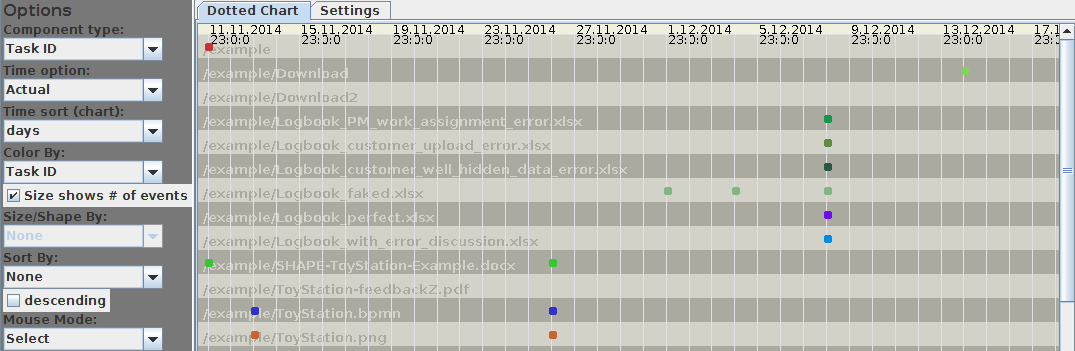
\includegraphics[width=\textwidth]{bpm2015/imgs/dotted_chart_ordered_by_taskID_cut}
\caption{Dotted chart from ProM}
\label{fig:dottedchart}
\end{figure}


\begin{figure}
\centering
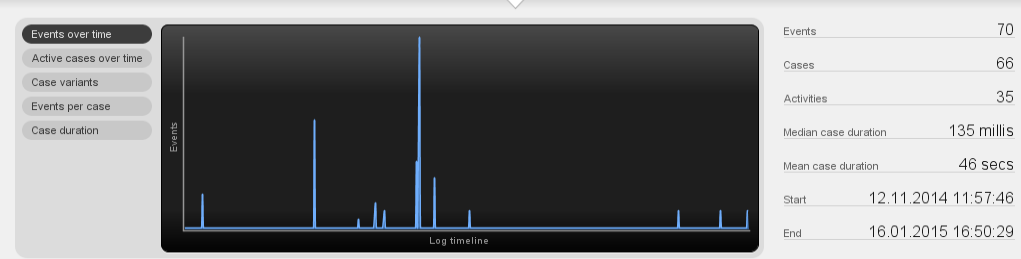
\includegraphics[width=\textwidth]{bpm2015/imgs/disco_screenshot_chart}
\caption{Chart from Disco plotting the events over time.}
\label{fig:discochart}
\end{figure}

Our approach to mining the work progress of project-oriented business processes complements these techniques with metrics and a corresponding visualization that is informative to managers.
\section{Conclusion}\label{sec:outro}

In this paper we
%identified a new a class of business processes that are executed according to planned data, resources and time constraints, to achieve predefined goals. We
addressed the problem of mining and visualizing project-oriented business processes in a way that is informative to managers. We define an approach that takes VCS logs as input to generate Gantt charts.
%provided a formal description to capture the project-oriented class of business processes. We presented an approach to mine them as Gantt charts from VCS logs.
Our algorithm works under the assumptions that repositories reflect the hierarchical structure of the project, each work package is contained in a corresponding directory and project members commit their work regularly during active working times.
The approach was implemented as a prototype and evaluated based on real-world data from open source projects.
%We implemented our method as a prototype tool that can visualize the project hierarchy along with events and activities for each level, by aggregation or disaggregation.
%Compared to classical process mining, our method offers a better overview on project structure and on the characteristics of work packages.
%Tests on real-world data, both from open source projects and from SHAPE, show how our metric on work packages can help to better understand work how efficiently they utilize their time.

In future work, we aim to extract further details of the VCS logs in order to calculate metrics that approximate the work effort. %\todo{Point 4 on the reviews: Add a discussion on how the project mining approach can is affected by different projects characteristics: number of commits, number of files, number of activities, duration of the project, number of participants, etc. } 
We plan to investigate on how the project mining approach is affected by project characteristics. Furthermore, we want to utilize statistical methods to better estimate the boundaries of the activities and work packages. Finally, we have already incorporated feedback from managers and plan to extend these to full user studies.

%from a more granular perspective, looking also into the parts of a file that were affected by a change. We also want to investigate ways that help us to better understand the boundaries of activities and work packages. We take into account using natural language processing techniques on the comments associated to commits and analyze their semantics. Furthermore, we want to consider clustering techniques in order to relax our assumptions on the directory structure.




\chapter{Uncovering the Hidden Co-Evolution in the Work History of Software Projects}

\todo[inline]{Link this solution to the existing problem. Say e.g. that the previous solution still lacks information about dependency. We would like to know what is inside a specific square in the BPM1 solution. As well, why some squares are connected.}

\todo[inline]{rephrase}

\abstract*{The monitoring of project-oriented business processes is difficult because their state is fragmented and represented by the progress
	of different documents and artifacts being worked on. This observation
	holds in particular for software development projects in which various
	developers work on different parts of the software concurrently. Prior contributions in this area have proposed a plethora of techniques to analyze
	and visualize the current state of the software artifact as a product. It is
	surprising that these techniques are missing to provide insights into what
	types of work are conducted at different stages of the project and how
	they are dependent upon another. In this paper, we address this research
	gap and present a technique for mining the software process including
	dependencies between artifacts. Our evaluation of various open-source
	projects demonstrates the applicability of our technique.}

The monitoring of project-oriented business processes is difficult because their state is fragmented and represented by the progress
	of different documents and artifacts being worked on. This observation
	holds in particular for software development projects in which various
	developers work on different parts of the software concurrently. Prior contributions in this area have proposed a plethora of techniques to analyze
	and visualize the current state of the software artifact as a product. It is
	surprising that these techniques are missing to provide insights into what
	types of work are conducted at different stages of the project and how
	they are dependent upon another. In this paper, we address this research
	gap and present a technique for mining the software process including
	dependencies between artifacts. Our evaluation of various open-source
	projects demonstrates the applicability of our technique.


\section{Monitoring the Work History of Software Projects}

\todo[inline]{rephrase}

In this section, we focus on a specific class of project-oriented business processes,
namely software development processes. These processes share some common
characteristics. First, they involve various resources with different roles. In the
simplest case, we can distinguish project managers and project participants.
Project managers are responsible for managing the development process and
supervising the work of the project participants, who in turn are responsible for
specific work tasks. Second, such processes are usually subject to constraints in
terms of cost, time and quality, which is mostly associated with the performance
of each of the work tasks. Third, the project participants work on a plethora of
artifacts, which are logically organized in a hierarchical structure, with complex
interdependencies among them. Given these characteristics, it is the goal of theproject manager to organize the software development process in such a way
that the work on different files and tasks reflects the complex interdependencies,
the constraints and the available participants. Therefore, it is important for the
manager to understand the work history of the process in order to monitor the
progress systematically.

This chapter is structured as follows. Section~\ref{sec:bpm2017background} describes the research problem along with its requirements and summarizes insights from prior research. Section~\ref{sec:bpm2017approach} presents our approach in detail. Section~\ref{sec:bpm2017evaluation} shows a prototypical implementation and evaluates its applicability both in a use case scenario and on real world projects from GitHub. Section~\ref{sec:bpm2017conclusion} concludes the paper.

\section{Approach to Monitoring Software Projects}

\todo[inline]{What has the state of the art done.}

\section{Related Work }
\label{sec:bpm2017background}
This thesis follows the \gls{dsr} paradigm~\cite{Peffers2008}. In this section, we describe the research problem in more detail and define requirements for a solution. Against these requirements, we analyze related work.
%and some background knowledge important for the understanding of our proposal.

%\subsection{Problem Description}
\label{subsec:prob-desc}
In this work, we focus on a specific class of project-oriented business processes, namely software development processes. These processes share some common characteristics. First, they involve various resources with different roles. In the simplest case, we can distinguish \emph{project managers} and \emph{project participants}. Project managers are responsible for managing the development process and supervising the work of the project participants, who in turn are responsible for specific work tasks. Second, such processes are usually subject to constraints in terms of cost, time and quality, which is mostly associated with the performance of each of the work tasks. Third, the project participants work on a plethora of artifacts, which are logically organized in a hierarchical structure, with complex interdependencies among them.
Given these characteristics, it is the goal of the project manager to organize the software development process in such a way that the work on different files and tasks reflects the complex interdependencies, the constraints and the available participants. Therefore, it is important for the manager to understand the \emph{work history} of the process in order to monitor the progress systematically.

%project specifies the tasks to be performed considering a hierarchy of files, within a limited period of time, and with a limited set of project participants, for achieving a specific goal, typically the release of a new version of a software. Best practices are often used to properly organize the work according, for instance, to good modularization principles. However, monitoring whether this or other guidelines are followed in the actual development process is not easy, due to the lack of an overarching process that defines the work.

%Project managers are interested in an understanding of the running project from a macro level. Useful information is concerns:
%\begin{inparaenum}[\itshape i)]
%	\item project structure;
%	\item profiles of users;
%	\item and the work history.
%\end{inparaenum} Existing tools in software development can help project managers to monitor and control these perspectives individually. For instance, CVS

%Nevertheless, these tools lack on information considering the work process reflected in the artifacts, i.e. artifact evolution, and a dependency among them beyond the structural provided by the hierarchy. Moreover, it is common to have hundreds of versions of thousands of files in a single project, which makes it impractical to browse this data manually.

\input{bpm2017/tables/vcs-data2}

Software tools like \glspl{vcs} do not provide direct support for monitoring work histories, but they provide a good starting point by continuously collecting event data on successive versions of artifacts.
%A starting point for analyzing software projects is represented by events that are stored in \glspl{vcs}, which help keeping track of successive versions of artifacts.
Table \ref{tab:vcs-log-data} shows an excerpt of log data, where the columns, from left to right, indicate the commit identifier, the project participant who committed the changes, the commit date, the comment written by the project participant and the files affected and the change performed\footnote{cf. unified diff format  \url{https://git-scm.com/docs/git-diff}}. In order to understand the work history and dependencies based upon such data, we identify three major requirements:

\begin{description}
	\item [R1 (Extract the work history):] Discover the process of how artifacts evolve in the project as a \emph{labeled} set of steps. This requirement is difficult because the version changes of a commit in relation to a single file do not directly reveal which type of work has been done. Both commit messages and edit characteristics might inform the labeling.	
	\item [R2 (Uncover Work-Related Dependencies):] Identify that certain work in one part of the project is connected with work in another part. This requirement is difficult because such dependencies might not only exist between files that reside in the same directory. For example, a change in a source code file might have the side effect of triggering work on a configuration file. We refer to this as \emph{co-evolution} of these files.
	\item [R3 (Measure Dependencies):] Determine how strong the co-evolution of different artifacts is. This requirement is difficult because measures of \emph{strength} of dependencies and on the \emph{distance} of   dependent artifacts have to be devised.
\end{description}


\subsection{Related Work}
\label{subsec:related}
A solution addressing these requirements can partially build upon research in three main areas:
\begin{inparaenum}[\itshape i)]
	\item work on \gls{msr};
	\item \gls{pm};
	\item and software visualization.
\end{inparaenum}

\input{bpm2017/tables/related-work-table}

Table~\ref{table:related-work} shows that these streams of research have mutual strengths, but no contribution covers the full spectrum. In general, methods from \gls{msr} have a strength in analyzing dependencies in the structure of the software artifact, but an explicit consideration of the type of work is missing. Contributions in this area focus on the users and the artifacts, mining co-evolution or co-change of project parts~\cite{zaidman2008mining,DAmbros2009} and network analysis of file dependency graph based on commit distance~\cite{Zimmermann2008,Abate2009,Weicheng2013}. Hidden work dependencies are mentioned as \emph{logical dependencies}~\cite{Oliva2011}. Also techniques for trend analysis~\cite{Ruohonen2015} and inter-dependencies between developers~\cite{lindberg2016coordinating} are proposed. However, none of these works considers the type of work being done in the process.

In the area of \gls{pm}, research gives more emphasis to the different tasks of the process. Some works focus on applying process mining for software repositories~\cite{Poncin2011a,Mittal2014,Bala2015}. In this context, approaches have been defined that use various queries to extract artifact evolution and resources~\cite{Beheshti2016,Beheshti2013}. There is research on identifying the tasks of the process by elicitation from unstructured data of user comments~\cite{Goncalves2011}. There are also process mining applications that focus on repetitive steps in software engineering, but not on singular project-oriented processes, such as \cite{Kindler2006}. All these works only consider the dependencies between work tasks to a limited extend.

%, but they lack a concept of work dependency. On the other hand, \gls{pm} contributions can help understand the work reflected by the artifacts, although to the best of our knowledge, a solution for hidden artifact dependencies is not existing yet. Moreover, \gls{pm} techniques are limited to recurrent work patterns (e.g., the process of bug fixing) and do not generally apply to the whole software project.

%In the area of \gls{msr}, many works analyze collaborative software development by mining \gls{vcs} log data.

There is also work in the area of software visualization. 
Visualization tools have been proposed in order to allow project managers to have a detailed overview of the software artifact being developed. These tools help to visually inspect artifacts similarities on different levels of granularity~\cite{Voinea2006b}, observe artifacts evolution or project members contribution~\cite{Ripley2007,Greene2015}. In general, they can be characterized as artifact-centric, and largely agnostic to the type of work being done.

%\Cref{table:related-work} summarizes how literature addresses the defined requirements. In general, methods from \gls{msr} are robust on analyzing dependencies in projects, but they lack a concept of work dependency. On the other hand, \gls{pm} contributions can help understand the work reflected by the artifacts, although to the best of our knowledge, a solution for hidden artifact dependencies is not existing yet. Moreover, \gls{pm} techniques are limited to recurrent work patterns (e.g., the process of bug fixing) and do not generally apply to the whole software project.

In the following, we develop a technique that addresses the three requirements and informs prior research on how to extract work histories and to identify the co-evolution of certain parts of a project-oriented software process.



%In this Section, we present closely related work to the approach proposed in this paper. We characterize closely related work as formal studies on providing method to extract or representing software development process. 
%
%Salameh et al. \cite{10.1109/CSIT.2016.7549475}  made a systematic review of literature to discuss Software Visualization and Evolution (SVE) tools and techniques. They analyzed 29 out of 55 papers. They concluded that the main source of information used by such tools is information extracted from software repositories. SVE tools can be classified into five different groups: graph-based, notation-based, matrix-based, metaphor-based and others. Graph-based are the most popular while notation-based are the least. SVEs focus can be either Artifact-centric visualization, Metric-centric visualization, Feature-centric visualization, or Architecture-centric visualization. The authors also identified generic functional requirements for software visualization tools: (i) views \cite{bani2016software}: show different representations; (ii) details-on demand: show more information/details; (iii) filter and search: show something conditionally; (iv) select: mark something as point of interest; (v) re-arrangement: show different arrangements of the data sets (e.g. sort, cluster, and aggregate); (vi) comparison: show the differences between different data sets.
%
%
%In \cite{Mittal:2014:PMS:2591062.2591152}, data achieved from four sources was evaluated: team wiki (used during requirement engineering), version control system (development and maintenance), issue tracking system (corrective and adaptive maintenance) and data generated as a result of constructing software by student teams in an educational setting. The main goal of the paper was to provide metrics and visualizations that better describe the work developed by the students in the discipline. From this analysis, it was possible to observe task distribution among the students in a project or commits behavior. 
%
%% Elsen \cite{DBLP:conf/vissoft/Elsen13} presents the prototype VisGi and a set of strategies for mining and displaying Git repositories. VisGi intends to abstract and visualize the branch structure of a Git, as well as its folder trees. By interpreting branches as groups of aggregated commits, their dependencies are condensed into a directed acyclic graph, and displayed using graph layout strategies. Tagging mechanisms are used to aggregate commits into compact nodes of a group graph. Sunburst diagrams are also proposed to display the content of the branches, the differences between each two branches, and the evolution of a particular selected path. Since the extraction is limited to the last commit of each group, it creates holes in older sections of most repositories. 
%
%%Greene and Fisher \cite{DBLP:conf/vissoft/Greene015} describe ConceptCloud, an interactive browser for SVN and Git repositories which combines an intuitive tag cloud visualization with an underlying concept lattice providing a formal structure for navigation. The authors claim that this solution can be used to answer questions such as \emph{What has happened in this project while I was away/?}, \emph{Which developers collaborate/?}, or \emph{What are the co-changed methods/?}. 
%
%In \cite{DBLP:conf/msr/RayNBNZ15}, Ray et al worry about improving risk analysis, recommendation and program repair techniques by automatic detecting unique changes in a software project history. They argue that unique changes require more expertise or represent code that is more complex or prone to mistakes than the more common similar (or non-unique) changes. Their contribution provides a valuable amount of information to support managers on the monitoring and managing software development processes; %however, they do not focus on visualization issues.
%
%Lehtonen et al.~\cite{DBLP:conf/ejc/LehtonenAKM16} proposed a visualization tool for collecting insights based on data collected through a tracking tool. The authors argue that analysis of this data helped the managers to understand the process more deeply showing what kind of spring lenghts and common deployment times actually exist and the identification of uncommonly long delivery times for some features. %Although the paper is related to ours in the sense that a visualization is proposed to help managers in a better decision making, in our work we focus on explicitin how the work is performed and how dependencies between artifacts combined with containments information can help understand how the development of the software can be improved.
%
%In \cite{Bala2015} a mining approach to help generate GANTT charts was proposed. They allow project managers to visualize work history from the perspective of activities performed inside a workpackage and the resource allocated to the activity.  Data from VCS logs are used for the mining and visualization. 
%
%Based on the literature proposals analyzed, we observed that solutions that deal with monitoring and managing software development process propose visualization tools that use data available from software repositories, version control systems, and IDEs [7]. Many tools have been proposed in order to support managers on the evolution of the software; They have similarities to ours, since it aims to provide insights about the project development to managers, however, they do not consider the files perspective. They do not analyses the evolution of each file over time and their relation, crossing information with structural information, like containments. Moreover, we also contribute presenting a story mining approach for automatically extracting the file evolution and provide representations of the knowledge extracted, thus facilitating the analysis of the managers, and crossing the gathered information.

%\subsection{Story Mining}
\label{subsec:story-mining}

%What is story mining and how we use it in our work
Gon\c{c}alves et al.~\cite{Goncalves2011} proposed a story mining approach to extract process elements from stories, i.e. text descriptions written collaboratively by the process participants. A story is a natural way to transmit and share knowledge. Using both natural language (text) and contextual elements (categorization of parts of the story), storytellers can express their experience and viewpoints about the work processes they participate, interact with and/or perceive. Stories have the advantage of reproducing the situations associated with their contexts - the knowledge that is difficult to capture in interviews or mining from Information Systems logs. Since collectively told, a story incorporates a range of perspectives. Business processes instances can also be viewed as stories played by individuals who perform specific roles depending on the circumstances.

Story Mining  \cite{Goncalves2011} receives as input a story freely written by the participants, describing their work in a particular business process. As an output, the \emph{actors} and the process \emph{activities} executed by them are extracted. To illustrate the approach consider the following story. The terms highlighted in {\bf bold} are the actors of the processes and the terms highlighted in {\color{gray} gray} the activities. 

\begin{figure}[!h]
{ \bf The system} {\color{gray} generates an estimating template consisting of the phases, activities and tasks} selected
for the project or project phase. When planning complete projects the estimating is typically done at the activity level, using the
list of tasks in the work breakdown as input to the estimating process. However {\bf estimators} will likely {\color{gray}add an itemized list of system functions and other deliverables}, to facilitate estimating the construction phase. {\bf Multiple estimators} {\color{gray} prepare estimates for each component}, {\color{gray}compare their estimates}, and {\color{gray}arrive at a final estimate} for each item.
  \label{RB}
\end{figure}

A further step that we developed in our approach is the identification of the relationship between the activities, therefore defining the flow.

\section{Conceptual Approach}
\label{sec:bpm2017approach}

%In this section, we describe our approach for mining software development projects. First, we give an overview of the approach itself, then we formally define concepts required by our technique.

%Version control systems (VCSs) are used in projects to ensure reliable collaboration.
%We build our technique on \gls{vcs}. In this context, project participants work on files (e.g., text, source code, spread sheets) and commit their changes to a central repository, which maintains information on the work history.

We propose a technique to extract and represent the work history and the dependencies among artifacts of a project-oriented business process. The technique takes as input a \gls{vcs} log and produces analysis data that describe the evolution of the artifacts, along with metrics about their distance and their similarity in terms of work.
The process is depicted in \Cref{fig:visualization-process} and consists of three successive steps towards extracting hidden work dependencies from \gls{vcs} event data. The method works under three main assumptions. First, we assume a \emph{meaningful tree structure}, i.e. the project participants organize the files in a representative hierarchy (e.g., spatially separating documentation from testing into different folders). Second, project participants perform \emph{regular commits} in the \gls{vcs}. Third, project participants write \emph{descriptive comments} that allow other members to understand the changes.

%\begin{itemize}
%	\item [A1:] {\bf Meaningful file tree structure.} The file tree structure in a project represents the structure of work of the project participants.
%	\item [A2:] {\bf Frequent commits.} Commits to the VCS are regularly performed.
%	\item [A3:] {\bf Meaningful comments.} The comments included by project participant when committing their work represent the changes done to the file being commit.
%\end{itemize}
%\vspace*{-.5cm}
\begin{figure}[h]
	\centering
	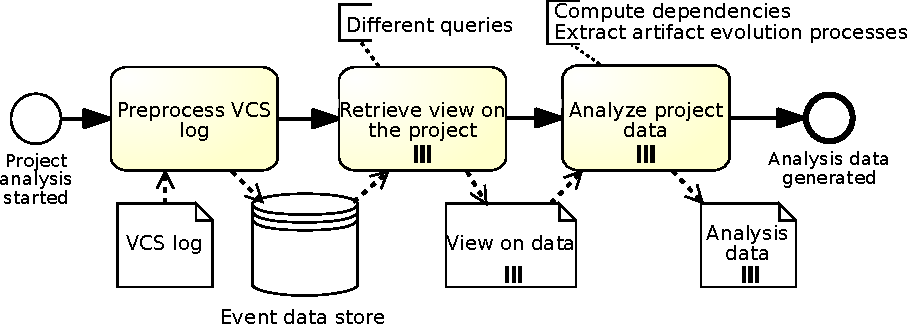
\includegraphics[width=.7\textwidth]{bpm2017/figures/visualization-process-crop}
	\caption[Approach for generating analysis data from VCS logs]{Approach for generating analysis data from VCS logs}
	\label{fig:visualization-process}
\end{figure}

The first step of the technique is the preprocessing of the \gls{vcs} log received as input. The main goal of this phase is to generate a set of events and store them into a database. Second, we obtain different views on the stored events. In particular, we are interested in observing
\begin{inparaenum}[\itshape i)]
	\item all the commits that affected the files over time;
	\item the amount of change brought by the commits to the files; and
	\item the users who issued such commits.
\end{inparaenum}
The third phase is responsible for considering the different perspectives defined by the project manager and through the generated views extract the necessary knowledge. In the following, we detail the formal concepts and the algorithm of our technique.



%We propose a techniques to extract and represent the work history and the dependencies among artifacts. The process is depicted in \Cref{fig:visualization-process} and consists of three successive steps towards extracting hidden work dependencies from \gls{vcs} event data. The method works under the following assumptions.

\begin{itemize}
\item [A1:] {\bf Meaningful file tree structure.} The file tree structure in a project represents the structure of work of the project participants.
\item [A2:] {\bf Frequent commits.} Commits to the VCS are regularly performed.  
\item [A3:] {\bf Meaningful comments.} The comments included by project participant when commiting their work represent the changes done to the file being commit.
\end{itemize}

\begin{figure}[h]
\centering
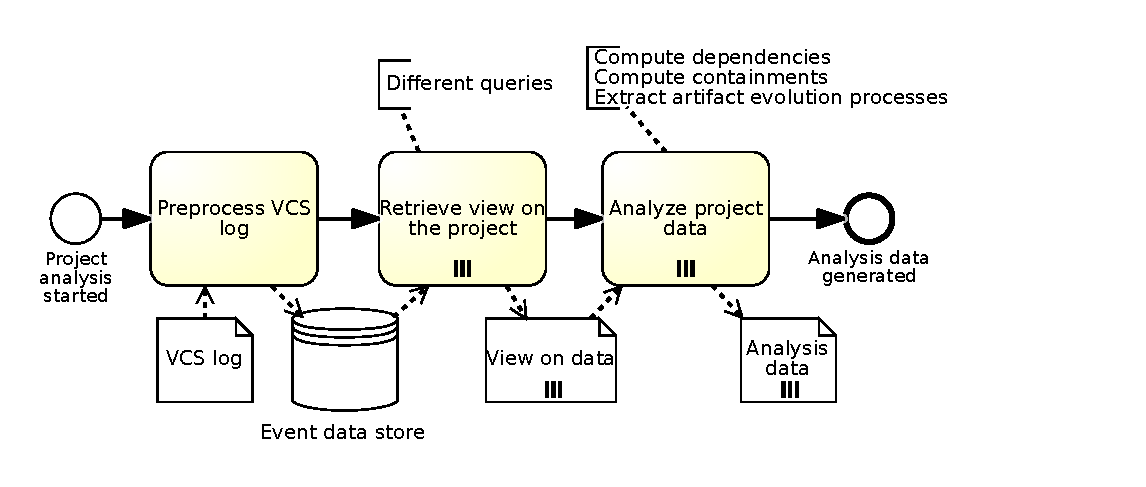
\includegraphics[width=.8\textwidth]{figures/visualization-process}
\caption[Generation of a process visualization from VCS logs]{Generation of a process visualization from VCS logs}
\label{fig:visualization-process}
\end{figure}

The first step of the approach is the preprocessing of the \gls{vcs} log received as input. The main goal of this phase is generate a set of events and store them into a database. Second, we obtain different views on the stored events. In particular, we are interested in observing
\begin{inparaenum}[\itshape i)]
	\item all the commits that affected the files over time;
	\item the amount of change brought by the commits to the files; and
	\item the users who issued such commits.
\end{inparaenum}
The third phase is responsible for considering the different perspectives defined by the project manager and through the generated views extract the necessary knowledge. The last phase is responsible for providing the visualization combining the different perspectives considered. In the following, we detail the formal concepts and the algorithm of our technique.

%\subsubsection{Preprocessing VCS Logs.}
%Version control system logs hold rich information about the artifacts and their evolution. Therefore, our process starts by extracting the elements \emph{Artifact}, \emph{Commit} and \emph{Event} from the log.
%
%First, the tree file is analyzed so the \emph{Parent} relation is defined. For that, the artifacts names appearing in the log are used. They provide the whole path from the root file until the leave file, which is the artifact in question. Thus, a parser can analyses the path and create the relation between the files. For instance, suppose we have the artifact \texttt{running example/software/model.java}. Three files are observed from this name: $f_1 = running \quad example$, $f_2 = software$ and $f_3 = model.java$. The following pairs will be included in the \emph{Parent} relation $\{(f_1,f_2),(f_2,f_3)\}$. 
%%are in the same containment if they share a common prefix that is maximal, i.e. they differ only by the name. For example, the files 
%%and \texttt{running example/software/test.java} . belong to the same containment, whereas the files  \texttt{running example/software/model.java} and \texttt{README.md} belong to two different containments. Note that containments can be contained in other containments, therefore every two files with eventually belong to the same containment. 
%
%Second, artifacts are extracted, as specified in Definition \ref{def_artifact}. Then the commits, following Definition \ref{def_commit}, are extracted. At last, the VCS raw log is transformed into a list of events for the extracted artifacts and commits, as specified in Definition \ref{def_event}. This step is easily done by replicating the information on commit level to be contained in the events. The amount of change is determined analyzing the attribute Diff of the VCS log. For instance, commit ID 2 in Table \ref{tab:vcs-log-data} indicates a commit with amount of change equals 3. The output of this phase is a set of events $E$, a set of artifacts $A$ and a set of commits $Com$.
%
%\subsubsection{Obtain View on Project.}
%The main goal of this phase is to extract the data that will be analyzed. The focus of this paper is in the artifacts, therefore the views generated gather information about events related to artifacts.  
%
%The project manager must determine the level of detail for the analyzes, thus, specifying the time windows. Input parameters of this phase are the interval of analysis ($ia$) and the time window for aggregation ($tw_{agg}$). Considering the specified $tw_{agg}$, the events generated in the previous phase are aggregated. For each artifact in a particular aggregate time an \emph{Aggregate Event} is generated as defined in Definition \ref{def_aggregateEvent}.
%
%\subsubsection{Analyze project data.}
%In this phase, the project is analyzed considering the different perspectives the project manager is interested in. In this paper, we considered three perspectives: dependency between artifacts, containments and artifact evolution.
%
%\paragraph{Dependency.} As stated in \Cref{def_dependency}, a dependency between two artifacts exists if both artifacts require a similar effort to be maintained, i.e. if they have a similar behavior considering the amount of changes.  The amount of change of an artifact over time defines  a time series. Therefore, for each artifact its aggregate events are analyzed in order to extract the amount of change for each aggregated time towards defining a time series for this artifact. 
%
%Let $AE$ be the set of aggregate events within $ia$. We build the time series for the \emph{i}-th artifact, namely $X_{f_i} = \lbrace (t, c) ~|~ e_a \in AE,~ t = ats(e_a),~ c = aac(e_a),~ f(e_a) = {f_i} \rbrace $. 
%
%%\todo[inline]{
%%Dependencies are obtained from the aggregated events. Considering the time window $tw$ and the aggregated event set in that time window ($AE_{tw}$), %$AE' = \lbrace e~|~ e \in AE,~ ts(e) \in tw \rbrace$,
%%we build the time series for the \emph{i}-th artifact, namely $X_{f_i} = \lbrace (t, c) ~|~ e_a \in AE_{tw},~ t = ats(e_a),~ t \in tw,~ c = aac(e_a),~ f(e_a) = {f_i} \rbrace $. As a result, the dependency between \emph{i}-th and the \emph{j}-th artifact is the correlation across time series $\sigma(i,j) = {corr(X_i, X_j)}$.
%%}
%
%After the time serie for each artifact is defined, the correlation function is used to calculate the correlation between the two time series. Considering artifacts $f_i$ and $f_j$ and the time series correspondent $X_{f_i}$ and $X_{f_j}$, $\sigma(f_i,f_j) = {corr(X_{f_i}, X_{f_j})}$ is the correlation value found when applying correlation function $corr$.
%
%If $\sigma(f_i,f_j)$ overcomes a threshold defined by the project manager (input parameter of this phase), then a dependency between the correspondent artifacts is established. The strength of the dependency is defined by $\sigma(f_i,f_j)$. 
%
%\paragraph{Containments.}
%For the containments extraction, the $Parent$ relation is analyzed and the set $C$ of containments defined.
%Containments reflect the hierarchical nature of the file structure in a repository. That is, \emph{composite containments} can be recursively decomposed into smaller containments until an \emph{atomic containment} is reached, following the tree structure of the file system top down. Conversely, from navigating the file structure bottom up, containments can be part of other containments until the root containment is reached. 
%
%
%\paragraph{Artifact evolution.}
%%For the artifact evolution definition, we propose to apply story mining techniques as follows.
%
%\input{sections/file-mining}

 %\hfill\\
%1. Compute correlation - dependency
%2. Compute containments 
%3. Apply story mining to obtain the process  - artifact evolution \\\hfill

%\subsubsection{Generate visualization.}
%%The approach is flexible making possible to generate different visualizations 
%In this section, we define the graphical elements of the visualization and their semantic. 
%
%%\input{table/visual-symbols}
%\paragraph{Project Participant.}
%%\todo[inline]{Task was not defined before. I think in our case workload will be in how many changes the project participant is involved within a period of time. I change to this idea. See what do you think. \\[2pt] I also consider project participant instead of resource following what was defined in section II.A. But I am ok with both. We just need to decide and change the whole paper. \\[2pt] The symbols have different faces and the semantic was not provided. I know they align with the color, but I think it is better to have the same face (not all people with high workload are sad or with low workload are happy). On the other hand, we lost the representation of a participant in the process, i.e. we are not able to visualize how many different participant worked in the same process (artifact). If we are still interested in that, I suggest to leave the faces as symbolizing the workload and the colors to symbolize different participants}
%
%Project Participants are displayed through a face symbol with its identification in the top, as depicted in  \Cref{fig:resources}. We use a color code to denote their level of workload, i.e. in how many changes the project participant is involved in the project within $ia$. \emph{Red}, \emph{yellow} and \emph{green} color indicate \emph{high}, \emph{medium} and \emph{low} project workload respectively. The project workload for a project participant ($wl_u$) is computed from the set of events in which the project participant was responsible for the change within $ia$, i.e. $wl_u(t_1,t_2) = |\lbrace e \in E ~|~  u(e)= u, t_1 \leq ts(e) \leq t_2 \rbrace|$, where $ia=[t_1 , t_2]$. These interval of analysis can be fine tuned to visualize the project participant occupancy over time. 
%
%%\begin{figure}[h]
%%	\centering
%%	\begin{subfigure}{.3\linewidth}
%%		\centering
%%		\begin{tikzpicture}[scale=.2]
%%		\node[text width=3cm] at (2,2.3) {resource};
%%		
%%		\filldraw [color=black, fill=green!50] (0,0) circle (2);
%%		\filldraw [color=black, fill=white] (-0.5,.6) ellipse (0.2 and 0.6);
%%		\filldraw [color=black, fill=white] (0.5,.6) ellipse (0.2 and 0.6);
%%		\filldraw [color=black, fill=black] (-0.5,.4) ellipse (0.2 and 0.3);
%%		\filldraw [color=black, fill=black] (0.5,.4) ellipse (0.2 and 0.3);
%%		\draw  (-1,-0.5) .. controls (-0.5,-1) and (0.5,-1) .. (1,-0.5);
%%		\draw  (-1,-0.5) .. controls (-0.5,-1.3) and (0.5,-1.3) .. (1,-0.5);
%%		\fill[fill=white, draw=black, opacity=1] (-1,-0.5) .. controls (-0.5,-1) and (0.5,-1) .. (1,-0.5) .. controls (0.5,-1.3) and (-0.5,-1.3) .. (-1,-0.5) --cycle;
%%		\end{tikzpicture}
%%		%		
\includegraphics[width=.3\linewidth]{figures/visualization-elements/green-face}
%%		\caption{}
%%		\label{fig:green}
%%	\end{subfigure}%
%%	\begin{subfigure}{.3\linewidth}
%%		\centering
%%		%		
\includegraphics[width=.3\linewidth]{figures/visualization-elements/yellow-face}
%%		\begin{tikzpicture}[scale=.2]
%%		\filldraw [color=black, fill=yellow!50] (0,0) circle (2);
%%		\filldraw [color=black, fill=white] (-0.5,.6) ellipse (0.2 and 0.6);
%%		\filldraw [color=black, fill=white] (0.5,.6) ellipse (0.2 and 0.6);
%%		\filldraw [color=black, fill=black] (-0.5,.4) ellipse (0.2 and 0.3);
%%		\filldraw [color=black, fill=black] (0.5,.4) ellipse (0.2 and 0.3);
%%		%mouth
%%		%		\draw  (-1,-0.6) .. controls (-0.5,-1) and (0.5,-1) .. (1,-0.5);
%%		%	\draw  (-1,-0.5) .. controls (-0.5,-1.3) and (0.5,-1.3) .. (1,-0.5);
%%		\fill[fill=white, draw=black, opacity=1] (-1,-0.7) .. controls (-0.5,-0.8) and (0.5,-0.8) .. (1,-0.7) .. controls (0.5,-1) and (-0.5,-1) .. (-1,-0.7) --cycle;
%%		\end{tikzpicture}
%%		\caption{}
%%		\label{fig:yellow}
%%	\end{subfigure}%
%%	\begin{subfigure}{.3\linewidth}
%%		\centering
%%		%		
\includegraphics[width=.3\linewidth]{figures/visualization-elements/red-face}
%%		\begin{tikzpicture}[scale=.2]
%%		\filldraw [color=black, fill=red!60] (0,0) circle (2);
%%		\filldraw [color=black, fill=white] (-0.5,.6) ellipse (0.2 and 0.6);
%%		\filldraw [color=black, fill=white] (0.5,.6) ellipse (0.2 and 0.6);
%%		\filldraw [color=black, fill=black] (-0.5,.4) ellipse (0.2 and 0.3);
%%		\filldraw [color=black, fill=black] (0.5,.4) ellipse (0.2 and 0.3);
%%		%			\draw  (-1,-0.5) .. controls (-0.5,-1) and (0.5,-1) .. (1,-0.5);
%%		%		\draw  (-1,-0.5) .. controls (-0.5,-1.3) and (0.5,-1.3) .. (1,-0.5);
%%		\fill[fill=white, draw=black, opacity=1] (-1,-1) .. controls (-0.5,-0.5) and (0.5,-0.5) .. (1,-1) .. controls (0.5,-0.8) and (-0.5,-0.8) .. (-1,-1) --cycle;
%%		\end{tikzpicture}
%%		\caption{}
%%		\label{fig:red}
%%	\end{subfigure}
%%	\caption{Project Participant symbols. Color codes represent the status of their workload within a period of time.}
%%	\label{fig:resources}
%%\end{figure}
%
%
%%\begin{figure}[h]
%%	\centering
%%		\begin{tikzpicture}[scale=.2]
%%		\node[] at (0,3.5) {\textit{participant}};
%%		\filldraw [color=black, fill=white!50] (0,0) circle (2);
%%		\filldraw [color=black, fill=white] (-0.5,.6) ellipse (0.2 and 0.6);
%%		\filldraw [color=black, fill=white] (0.5,.6) ellipse (0.2 and 0.6);
%%		\filldraw [color=black, fill=black] (-0.5,.4) ellipse (0.2 and 0.3);
%%		\filldraw [color=black, fill=black] (0.5,.4) ellipse (0.2 and 0.3);
%%		%mouth
%%		%		\draw  (-1,-0.6) .. controls (-0.5,-1) and (0.5,-1) .. (1,-0.5);
%%		%	\draw  (-1,-0.5) .. controls (-0.5,-1.3) and (0.5,-1.3) .. (1,-0.5);
%%		\fill[fill=white, draw=black, opacity=1] (-1,-0.7) .. controls (-0.5,-0.8) and (0.5,-0.8) .. (1,-0.7) .. controls (0.5,-1) and (-0.5,-1) .. (-1,-0.7) --cycle;
%%		\end{tikzpicture}
%%	\caption{Project Participant symbol. The workload within a period of time is color coded.} 
%%	\label{fig:resources}
%%\end{figure}
%
%
%
%\paragraph{Dependency.}
%A dependency between two artifacts is represented by a line that connects their atomic containments. We label dependencies with a number  $\sigma \in \Re$, which indicates the strength of the dependency among the two artifacts. \Cref{fig:dependency} illustrate the notation for dependencies.
%
%%\begin{figure}[h]
%%	\centering
%%	%	
\includegraphics[width=0.7\linewidth]{figures/visualization-elements/dependency}
%%	\begin{tikzpicture}[scale=.5]
%%	\draw[thick] (-2,0) -- node[above,thick] {$\sigma$} ++(4,0);
%%	\end{tikzpicture}
%%	\caption{Dependency with strength $\sigma$}
%%	\label{fig:dependency}
%%\end{figure}
%
%\paragraph{Artifact evolution.}
%
%The artifact evolution is a process under which the artifact changes step by step towards a final state reached eventually in the project (e.g. a documentation file reaches his final state when the documentation is complete and no edits are made to that version of document anymore). Thus, we chose the \gls{bpmn} to represent this process. 
%
%\Cref{fig:process} depicts an example of a process learned considering a story with two aggregated comments, thus a process with two sequential activities \emph{a} and \emph{b}, modeled in \gls{bpmn}. 
%
%%\tikzstyle{startstop} = [rectangle, rounded corners, minimum width=1.5cm, minimum height=1cm,text centered, draw=black, fill=white!30]
%%\tikzstyle{arrow} = [thick,->,-latex]
%%\tikzstyle{event} = [circle,scale=.5, minimum width=1cm, minimum height=1cm,draw,fill=white]
%%\tikzstyle{end event} = [event,ultra thick]
%%
%%\begin{figure}[h]
%%	\centering
%%	%
\includegraphics[width=0.7\linewidth]{figures/visualization-elements/process}
%%	\begin{tikzpicture}[scale=.3]
%%	\begin{scope}[auto, every node/.style={draw,circle},node distance=.2cm]
%%	\node (start) [event] {};
%%	\node (add) [startstop, right of=start, xshift=1.3cm] {a};
%%	\node (fix) [startstop, right of=add, xshift=1.9cm] {b};
%%	\node (end) [end event, right of=fix, xshift=2.8cm] {};
%%	\draw [arrow]  (start) -- (add);
%%	\draw [arrow]  (add) -- (fix);
%%	\draw [arrow]  (fix) -- (end);
%%	\end{scope}
%%	\end{tikzpicture}
%%	\caption{Process representing an artifact evolution using \gls{bpmn}.}
%%	\label{fig:process}
%%\end{figure}
%
%
%\paragraph{Containment.} 
%A containment is represented with a rectangle. 
%We overload the semantic of rectangle used to represent the containment with a time concept. The position of the \emph{atomic containments} is shifted within the boundaries of their parent containments according to the first timestamp of the artifact history. For example, given two \emph{atomic containments} $C_1\{f_i\}$, $C_2\{f_j\} \subseteq C$, and let $AE_i, AE_j \subseteq AE$ be the sets of aggregated events that affected these artifacts, respectively. Then $C_1$ is shifted left with respect to $C_2$ if $min\{ats(e) | e \in AE_i\} < min\{ats(e') | e' \in AE_j\}$. \Cref{fig:containment} illustrates this example.
%
%%\begin{figure}[h]
%%\centering
%%%
\includegraphics[width=0.7\linewidth]{figures/visualization-elements/containment}
%%\usetikzlibrary{
%%	shapes.geometric,
%%	positioning,
%%	fit,
%%	calc
%%}
%%\begin{tikzpicture}
%%	\draw[thick] (0,0)rectangle (4,2) node[pos=.85] {$C_3$};
%%	\draw[thick] (1.1,1.1) rectangle (2.2,1.6) node[midway] {$C_1$}; 
%%	\draw[thick] (2.1,0.1) rectangle (3.2,0.6) node[midway] {$C_2$};
%%\end{tikzpicture}
%%\caption{A containment $C_3$ composed of two atomic containments $C_1$, $C_2$. $C_1$ is shifted more left wrt $C_2$ as its contained artifacts were affected by changes earlier.}
%%\label{fig:containment}
%%\end{figure}
%
%\begin{figure}
%	\centering
%	\begin{subfigure}[t]{.5\textwidth}
%		\centering
%		\begin{tikzpicture}[scale=.2]
%		\node[] at (0,3.5) {\textit{participant}};
%		\filldraw [color=black, fill=white!50] (0,0) circle (2);
%		\filldraw [color=black, fill=white] (-0.5,.6) ellipse (0.2 and 0.6);
%		\filldraw [color=black, fill=white] (0.5,.6) ellipse (0.2 and 0.6);
%		\filldraw [color=black, fill=black] (-0.5,.4) ellipse (0.2 and 0.3);
%		\filldraw [color=black, fill=black] (0.5,.4) ellipse (0.2 and 0.3);
%		%mouth
%		%		\draw  (-1,-0.6) .. controls (-0.5,-1) and (0.5,-1) .. (1,-0.5);
%		%	\draw  (-1,-0.5) .. controls (-0.5,-1.3) and (0.5,-1.3) .. (1,-0.5);
%		\fill[fill=white, draw=black, opacity=1] (-1,-0.7) .. controls (-0.5,-0.8) and (0.5,-0.8) .. (1,-0.7) .. controls (0.5,-1) and (-0.5,-1) .. (-1,-0.7) --cycle;
%		\end{tikzpicture}
%		\caption{Project Participant symbol. The workload within a period of time is color coded.} 
%		\label{fig:resources}
%	\end{subfigure}~
%	\begin{subfigure}[t]{.5\textwidth}
%		\centering
%		%	
\includegraphics[width=0.7\linewidth]{figures/visualization-elements/dependency}
%		\begin{tikzpicture}[scale=.5]
%		\draw[thick] (-2,0) -- node[above,thick] {$\sigma$} ++(4,0);
%		\end{tikzpicture}
%		\caption{Dependency with strength $\sigma$}
%		\label{fig:dependency}
%	\end{subfigure}\\
%	\begin{subfigure}[t]{.5\textwidth}
%		\tikzstyle{startstop} = [rectangle, rounded corners, minimum width=1.1cm, minimum height=.6cm,text centered, draw=black, fill=white!30]
%		\tikzstyle{arrow} = [thick,->,-latex]
%		\tikzstyle{event} = [circle,scale=.7, minimum width=.5cm, minimum height=.5cm,draw,fill=white]
%		\tikzstyle{end event} = [event,ultra thick]
%		%		\begin{figure}[h]
%		\centering
%		%
\includegraphics[width=0.7\linewidth]{figures/visualization-elements/process}
%		\begin{tikzpicture}
%		\begin{scope}[auto, every node/.style={draw,circle},node distance=.05cm]
%		\node (start) [event] {};
%		\node (add) [startstop, right of=start, xshift=1cm] {a};
%		\node (fix) [startstop, right of=add, xshift=1.5cm] {b};
%		\node (end) [end event, right of=fix, xshift=1.6cm] {};
%		\draw [arrow]  (start) -- (add);
%		\draw [arrow]  (add) -- (fix);
%		\draw [arrow]  (fix) -- (end);
%		\end{scope}
%		\end{tikzpicture}
%		\caption{Process representing an artifact evolution using \gls{bpmn}.}
%		\label{fig:process}
%		%		\end{figure}
%	\end{subfigure}~~
%	\begin{subfigure}[t]{.45\textwidth}
%		\centering
%		%
\includegraphics[width=0.7\linewidth]{figures/visualization-elements/containment}
%		\usetikzlibrary{
%			shapes.geometric,
%			positioning,
%			fit,
%			calc
%		}
%		\begin{tikzpicture}[scale=.99]
%		\draw[thick] (0,0)rectangle (4,2) node[pos=.85] {$C_3$};
%		\draw[thick] (1.1,1.1) rectangle (2.2,1.6) node[midway] {$C_1$}; 
%		\draw[thick] (2.1,0.1) rectangle (3.2,0.6) node[midway] {$C_2$};
%		\end{tikzpicture}
%		\caption{A containment $C_3$ composed of two atomic containments $C_1$, $C_2$. $C_1$ is shifted more left wrt $C_2$ as its contained artifacts were affected by changes earlier.}
%		\label{fig:containment}
%	\end{subfigure}
%	\caption{Graphic elements used to represent the defined concepts of project participant, work dependency, artifact evolution and containment.}
%\end{figure}
%
%\paragraph{Composing the visualization.}
%
%The layout rules to compose the visualization are the following. 
%\begin{inparaenum}[\itshape (i)]
%	\item Every element is within a containment, excluding the root;
%	\item Project participants responsible for the change are placed over \gls{bpmn} activities;
%	\item Artifact evolution is within an atomic containment;
%	\item Dependencies connect atomic containments, showing the strength of correlations between the belonging artifacts evolutions.
%\end{inparaenum}
%\Cref{fig:all-elements-together} shows the correct composition of the presented visual elements.
%
%\begin{figure}
%\centering
%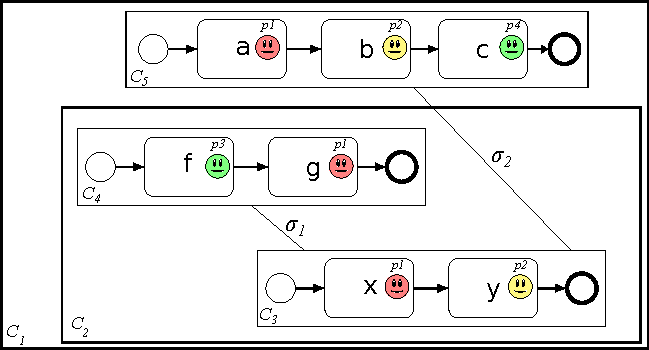
\includegraphics[width=.6\linewidth]{figures/visualization-elements/al-elements-together}
%\caption{Composition of the graphic elements into five containments, of which two are composite.}
%\label{fig:all-elements-together}
%\end{figure}



\subsection{Preliminaries}
\label{subsec:prelim}

%1. How we define/capture software processes\\

%2. How we define containment\\

%3. How we define dependencies\\

%Version control systems (VCSs) are used in projects to ensure reliable collaboration. We build our technique on \gls{vcs}. Typically, people work in VCS on files (e.g., text, source code, spread sheets) and commit them to the central repository. Project participants comment on their commits so that other participants can better understand the nature of the changes performed to the files.

As the objective of our technique is to uncover hidden work dependencies, we define the fundamental concepts required to capture them. Work is reflected by \emph{artifacts}, e.g., word documents, spreadsheets, code, etc. Artifacts are leaves in the file tree hierarchy (with directories being special type of non-leaf files). %Each directory in the file system groups together one or more files into a so-called \emph{containment}. 
Artifacts evolve over time, while project participants contribute their changes. Each change is an \emph{event} that happens to an artifact in a single point in time. Events can be abstracted into \emph{aggregated events} that allow a coarser grained view on the history. The history of the changes of an artifact over a time interval at a given level of abstraction is referred to as \emph{artifact evolution}. Similar artifact co-evolution establishes a \emph{dependency} between two artifacts. %In the following, we formally define the aforementioned concepts.

A software product is subdivided into files and directories. In this work, we consider directories as special type of files which are parents of other files. Formally, let $F$ be the universe of files in a software development project. Files are organized in a file tree. Therefore, each file $f \in F$ has one parent file. The only file without a parent file is the \emph{root} file. We capture this information in the parent relation $Parent: F \times F$. For example, let $f_p \in F$ be the parent of file $f_c \in F$, then $(f_p, f_c) \in Parent$. %Every file in $Parent$ defines a so-called \emph{containment}. For example, let $Parent = \{(f_{p_1} , f_{c_1})$, $(f_{p_1},f_{c_2})$, $(f_{p_2},f_{c_3})$, $(f_{p_3},f_{p_1})$,$(f_{p_3},f_{p_2})\}$, then files $f_{p_1}$, $f_{p_2}$ and $f_{p_3}$ define containments. Let $C$ be the set of containments. In our example $C=\{f_{p_1}, f_{p_2}, f_{p_3}\}$.
An \emph{artifact} is a file that is not a parent file, i.e. a file $f_a$ is an artifact if $\forall_{f \in F} (f_a, f) \notin Parent$.

%In this work, we are interested in describing the work progress related to a specific file, that we henceforth call \emph{artifact} and describe as follows:

%\begin{definition}
%	\label{def_artifact}
%	{\bf (Artifact)} An \emph{artifact} is a file that it is not a parent file, i.e. a file $f_a$ is an artifact if $\forall_{f \in F} (f_a, f) \notin Parent$.
%\end{definition}
%
%The files are grouped considering their organization in the tree file. We call each of these groups \emph{containments} and they are defined as follows:
%\begin{definition}
%\label{def_containment}
%{\bf (Containment)} A \emph{containment} is a file that is a parent of at least one other file. For example, let $Parent = \{(f_{p_1} , f_{c_1})$, $(f_{p_1},f_{c_2})$, $(f_{p_2},f_{c_3})$, $(f_{p_3},f_{p_1})$,$(f_{p_3},f_{p_2})\}$, then files $f_{p_1}$, $f_{p_2}$ and $f_{p_3}$ are containments. Let $C$ be the set of containments. In our example $C=\{f_{p_1}, f_{p_2}, f_{p_3}\}$.
%\end{definition}

%\begin{definition}
%	\label{def_artifact}
%	{\bf (File Containment)} An \emph{artifact} is a file that it is not a parent file, i.e. a file $f_a$ is an artifact if $\forall_{f \in F} (f_a, f) \notin Parent$.
%\end{definition}


%Containments can be either \emph{atomic} or \emph{composite}. An \emph{atomic containment} is a file which is parent of artifacts. In our example, containments $f_{p_1}$ and  $f_{p_2}$ are atomic containments.
%%\Cref{fig:containment} shows the visual symbol for an atomic containment.
%A \emph{composite containment} is a containment which is not atomic, i.e. it involves files which are parents of parents. In our example, containment $f_{p_3}$ is a \emph{composite containment}.  Therefore, the set $C$ of containments is partitioned in two subsets $C=C_1 \cup C_2$. In our example, $C=\{\{f_{p_1}, f_{p_2}\},\{f_{p_3}\}\}$.


% are defined, $C_1 = \{f_{c_1},f_{c_2}\}$ and $C_2=\{f_{c_3}\}$. A \emph{containment} $C$ is a set of files with the same parent file. For example, let $Parent = \{(f_{p_1} , f_{c_1}), (f_{p_1},f_{c_2}), (f_{p_2},f_{c_3})\}$, then two containments are defined, $C_1 = \{f_{c_1},f_{c_2}\}$ and $C_2=\{f_{c_3}\}$.

When project participants do a certain amount of work and want to save their current progress, they commit the changes to the \gls{vcs}. We define changes on artifacts as the \emph{events} of interest on the lowest granularity.

\begin{definition} {\bf(Event)}
\label{def_event}
Let $E$ be the set of events. An \emph{event} $e \in E$ is a five-tuple $(f, ac, ts, k,u)$, where
\begin{itemize}
\item $f \in F$ is the affected artifact of the event.
%\item $o \in O$ = \{added, modified, deleted\} is the change operation on the artifact with obvious meaning.
\item $ac \in AC =  \mathbb{N}$ is the amount of change done in the artifact.
\item $ts \in TS = \mathbb{N}$ represents a unix time stamp marking the time of the event occurrence.
\item $k \in \Sigma ^* $ is a comment in natural language text.
\item $u \in U$ is the project participant responsible for the change.
\end{itemize}
\end{definition}

For event $e = (f, ac, ts, k,u)$ we overload $f$, $ac$, $ts$, $k$ and $u$ to be used as accessor functions. For example, $f$ is the function $f : E \rightarrow F$ mapping an event to its affected artifact.

In some situations, it can be interesting to have a higher level overview of the changes done to a particular artifact. In this case, an aggregation of events related to this artifact in an interval of time can be performed. The time window for the aggregation, henceforth denoted as $tw_{agg}$, must be defined, i.e. the size of the time interval. For instance, a time window for aggregation can be a day. Thus, all events occurring for an artifact in the same day will be aggregated. An \emph{aggregated event} is defined as follows:

\begin{definition} {\bf (Aggregated Event)}
\label{def_aggregateEvent}
An \emph{Aggregated Event} for $tw_{agg}$ ($AE_{tw_{agg}}$) is a five-tuple $(f, aac, ats, ak,au)$, where
\begin{itemize}
\item $f \in F$ is the affected artifact in the set of events being aggregated.
%\item $ao \in O$ = \{added, modified, deleted\} is the aggregated change operation on the artifact. If the only change operation performed in $tw_{agg}$ was \emph{added} or \emph{deleted} then the aggregated change operation is the same, otherwise it is \emph{modified}.
\item $aac \in AAC =  \mathbb{N}$ is the aggregate amount of change done in the artifact for $tw_{agg}$. It is calculated by summing the amount of changes done in each of the time aggregated.
\item $ats \in ATS = \mathbb{N}$ represents an aggregate time of the unix time stamp of the events being aggregated.
\item $ak \in \Sigma ^* $ is the concatenation of the comments presented in the events being aggregated.
\item $au \subseteq U$ are the project participants responsible for the changes in $tw_{agg}$ being aggregated.
\end{itemize}
\end{definition}
%\todo[inline]{We consider a $tw$ but do not use it in the definition.}

The set of aggregated events for a particular artifact defines how this artifact evolves over time. Considering an interval of analysis, henceforth denoted as $ia$, we define artifact evolution as follows.

\begin{definition} {\bf (Artifact Evolution)}
%Let $EA_f$ be the set of all aggregated events related to artifact $f$.
\emph{Artifact evolution} is the process describing how the file $f$ changed over an interval of time $ia$, i.e., a set of labeled tuples $A_{evo}(f) = \{ (t,a,l) | e \in AE_{ia}, f=f(e), t=ats(e), a=aac, l=ak(e)\}$ chronologically ordered.

%The comments associated to the aggregated events in $EA_f$ define the activities executed. The time of the aggregated events in $EA_f$ establishes the order of the activities and then the flow of evolution. Each activity is associated with the user that executed it.
\end{definition}

%Project participants can commit a number of changes to different artifacts at one step. Therefore, we define the notion of commits as follows.
%
%\begin{definition} {\bf (Commit)}
%\label{def_commit}
%A \emph{commit} $Com$ is a set of events sharing the same time stamp and comment, i.e., $\forall e, e'\in Com : ts(e) = ts(e')\wedge k(e) = k(e')$. Additionally, each event in a commit affects different artifact, i.e., $\forall e, e' \in Com : e \neq e' \rightarrow f(e) \neq f(e')$.
%\end{definition}

%For example, a dependency is established if the two artifacts require a similar effort to be maintained. The effort of maintenance is measured through the amount of changes done to the artifact.

%\begin{definition} {\bf (Dependency)}
%\label{def_dependency}
%A \emph{dependency} between two artifacts within $ia$ is a similarity function $\sigma : X_{evo} \times X_{evo} \rightarrow \mathbb{Z}$, where the artifact evolution set in which the labels are projected out, i.e $X_{evo} = \{(t,a) | \exists l : (t,a,l) \in A_{evo}\}$.
%%Thus, each artifact defines a time series of the amount of change. If the correlation between two time series is significant then a dependency between the correspondent artifacts is established. The strength of the dependency is defined by the correlation value.
%\end{definition}
%
%
%
%\subsection{Metrics} 

Note that artifact evolution represents the changes that happened to a file over time. Thus, we can build the time series of a file $f$ as the vectors of changes $\vec{X_{f}} = (a_1, ..., a_n)$ in the time window $tw_{agg} = [t_1,t_n]$, with $a_i$ being the sum of the changes of $f$ in of the aggregated intervals $t_i$ of the time window $tw_{agg}$.

%The file system establishes a structural tree-based relationship among files. However, other types of dependencies can emerge between two files. In this paper, we define dependency between two files in terms of their \emph{degree of co-evolution}.
%In this paper, we are interested in measuring the hidden work-dependencies among artifacts of the project-oriented business process. That is, we want to capture dependencies that are created among files that go beyond functional (e.g. interface-implementing class) or structural (e.g., parent-child in the file tree structure).

%We define the metrics of \emph{degree of co-evolution} and \emph{file distance}. 

We measure the dependency between two files $f_a$ and $f_b$ in terms of their \emph{degree of co-evolution} as follows.
\begin{definition} {\bf (Degree of Co-Evolution)} 
	\label{definition:degree-of-coevolution}
	Given two files $f_a$ and $f_b$, the \emph{degree of co-evolution} $\chi: F \times F \rightarrow [0,1]$ is a similarity function of the respective time series.
\end{definition}
In this paper, we fix $\chi(f_a,f_b) = |\sigma (\vec{X_{f_a}}, \vec{X_{f_b}})|$, where $\sigma$ is the correlation function of the two vectors $\vec{X_{f_a}}$ and $ \vec{X_{f_b}}$.

The way files are kept in the directory structure establishes an inherent relationship among files being stored close to each other in the hierarchy. For instance, files serving the same purpose are stored close to each other in the file system. 
Hidden work dependencies are expected to happen between artifacts that are distant in the file structure. We measure this distance as the length of the shortest route connecting two files in the file tree. We adapt the notion of path from~\cite{Gubichev2010} to our file tree. Given a file $f$, the path to the root node can be obtained by navigating the $Parent$ relationship up to the root file. The path $p$ from $f_a$ to the root $f_r$ is the set of parent files encountered along such route. i.e. $p(f_1,f_{r}) = \{(f_1, ..., f_k, f_{k+1}, ..., f_{r})\}$ such that for any $k$, $(f_{k+1},f_k) \in Parent $. The length of the path is the cardinality $|p|$ of the set. 
The shortest path between two files $f_a$, $f_b$ in a tree passes through the \gls{lca}~\citep{Bender2000}. This is equivalent to considering the paths from the single files to the root node $p_a = p(f_a,f_r)$ and $p_b=p(f_b, f_r)$ minus their intersection $I_{p_a,p_b}=\{p(f_a, f_r) \cap p(f_b, f_r)\}$. Thus, we define the \emph{file distance} as the length of the shortest path between two files $f_a$ and $f_b$ as follows. 

\begin{definition} {\bf (File Distance)} 
	\label{definition:artifact-distance}
	The distance $d : F \times F \rightarrow \mathbb{N} $ between two files belonging to the same directory structure is defined as the number of nodes in the minimum path connecting the two files in the project file tree: $d(f_a,f_b) =  |p_a| + |p_b| - 2*(|I_{p_a,p_b}|)$.
\end{definition}
 

\subsection{Hidden Dependencies Discovery Algorithm}

We are focused on finding interesting hidden work dependencies. These dependencies are typically reflected by changes that happen to couples of allegedly unrelated files during their evolution. This section details the procedure that implements the technique outlined in \Cref{fig:visualization-process}.

\Cref{algorithm:all} presents the steps required to explicate such hidden dependencies. The procedure $\mathtt{PreprocessLog(\mathcal{L})}$ in line~\ref{step:preprocess} takes as input a VCS log $\mathcal{L}$ structured as in \Cref{tab:vcs-log-data} and parses out work events at the granularity of line changes. These events are then stored into an event data storage. Events parsed from \gls{vcs} logs contain rich information about multiple aspects of the work they reflect. In order to represent all these different aspects, we devised the entity-relationship data model. Hence, we are able to store all the information that is possible to obtain after parsing the \gls{vcs} log. Furthermore, this step allows the user to obtain simple information, such as statistics on the project, already at an early stage of the procedure. The output of the $\mathtt{PreprocessLog(\mathcal{L})}$ step results in the storage of all the events $E$ into a database.
%Further on, we will show a possible implementation that uses a database to store the parsed events, but in principle any type of repository that allows to store the preprocessed events can be considered.

%\begin{figure}
%	\centering
%	\includegraphics[width=.8\textwidth]{figures/CommitLogER3.pdf}
%	\caption{Entity-Relationship model used to store events extracted from VCS logs}
%	\label{fig:data-model}
%\end{figure}


Next, the iterative call of the procedure $\mathtt{RetrieveView(\mathit{E}, \mathsf{query})}$ in line \ref{step:retrieve-view} performs several querying the data storage containing the set $E$. For example, a possible query can obtain all the comments associated to each change of a specific file. To obtain information on the evolution of files, we query the database for the changes of all the files within a user defined time interval $tw_{agg}$. In general several time frames can be chosen, each of them producing a \emph{view} $V$ on the data, i.e., a set of aggregated events chronologically sorted within $tw_{agg}$. For example, users may be interested in artifact-views aggregated by day, by month, etc. Multiple \emph{views} are possible by defining them in the {\textsf{queries}} parameter. We collect these views into a set $\mathcal{V} = \bigcup_{\textsf{queries}} V$. 

%Step~\ref{step:contaiments} extracts the structural relationships among the file paths contained in each view $V$, i.e., it recreates the file tree from the artifacts.


\input{bpm2017/algorithms/all}%\input{algorithms/RetrieveView}
%\Cref{algorithm:compute-containments} computes the containments. Note that both atomic and composite containments are computed.

%\input{algorithms/ComputeContainments}

The step in line~\ref{step:evolution} starts an iteration over the views set $\mathcal{V}$. Here is where we collect the analysis data that are returned by the algorithm. For each of the aggregated artifacts contained in a view $V$, we retrieve the information necessary to compute the \emph{degree of co-evolution} between pairs of files and their \emph{file distance}. First, we construct the artifact evolution of all the artifacts present in $ae \in V$. 
Note that an aggregated event $ae \in V$ is a record obtained from a view on the project which is composed, among other attributes (e.g., file, time, amount of change), by the comment associated to the specific change. Comments describe multiple changes executed on the file, i.e. they describe a \emph{story} of the artifact. 
Stories associated to each file are collected and the corresponding labels are chronologically ordered. These file stories are then input to the StoryMining technique~\citep{Goncalves2011}. Story Mining was designed to receive as input a story freely written by the participants, describing their work in a particular business process. As an output, the \emph{actors} and the process \emph{activities} executed by them are extracted. Our technique is concerned with the stories of the files. Therefore, they are the actors of the story mining, and the resulting business process consists of the steps describing their evolution process. We collect the resulting processes in the step in line~\ref{step:story-mining}.
The step in line~\ref{step:timeseries} is concerned with the construction of a time series from the set of artifact evolutions $A_{evo}$ computed in line~\ref{step:a-evo}. Specifically, this step gathers the values of the changes of each of the artifact $f$ in $A_{evo}$ and records them in $TimeSeries(f)$. 

After all the aggregated events $ae$ have been explored, the algorithm moves on to computing the metrics (lines~\ref{step:metric-start}--\ref{step:metric-end}). In this loop, the algorithm iterates through all the pairs of files. For each pair, the \emph{degree of co-evolution} and \emph{artifact-distance}  metrics are computed according the \Cref{definition:degree-of-coevolution} and \Cref{definition:artifact-distance}, respectively. These two measures are collected only if their values are above the user defined thresholds $\gamma$ and $\delta$. After the loop is over, the two measurements and the stories mined with the StoryMiner are stored in $AnalysisData$.

Finally, after iterating over all the user defined views, the algorithm returns the $AnalysisData$ collection which can now be further inspected and analyzed in more detail, as we show next with an example.

%\input{algorithms/ComputeEvolution}



%\input{algorithms/ComputeDependencies}
%
%The algorithm iterates over the views and creates the time series from the aggregated events $v$ in each of the views $V$ of the view collections $\mathcal{V}$. A time series is captured by a set $X_{f_i}$, recording the trend of the changes of file $f_i$ over the time. Next, the dependencies are calculated by using the similarity function $\sigma$ (cf. \Cref{def_dependency}) pairwise over the time series of the different artifacts. We do not enforce a determined similarity function between time series. The user can adopt a customized time series similarity function or use an existing method from literature (e.g.~\cite{ruohonen2015time}). Because the time series must have equal length, we add missing times $t$ with couples $(t,0)$. These couples denote that the amount of change in $f$ at time $t$ was 0. Finally, we collect the results in the dependencies set $D$ if they are stronger than the threshold $\delta$.



%\subsection{Metrics}

We are interested in measuring the hidden work dependencies among artifacts of the project-oriented business process. Therefore we define the metrics of \emph{degree of co-evolution} and \emph{file distance}. The degree of co-evolution is used to indicate dependency relations between files. We focus on the similarity of the evolution between two files $f_a$ and $f_b$. We build the time series for each of the files as the vectors of changes over time $\vec{X_{f_a}} = (c_1^a, ..., c_n^a)$ and $\vec{X_{f_b}} = (c_1^b, ..., ,c_n^b)$, where the indexes of $i \in [1,n]$ are of the corresponding aggregated time event in the time windows $tw_{agg} = [t_1,t_n]$, and $c_i^j$ are the changes in the aggregated period $t_i$ of the file $f_j$. We measure the co-evolution of two artifacts as the absolute value of the correlation $\sigma(f_a,f_b)$ of the respective time series.

\begin{definition} {\bf (Degree of Co-Evolution)} 
	\label{definition:degree-of-coevolution}
	The \emph{degree of co-evolution} is a function $\chi: F \times F \rightarrow [0,1]$. 
	\[
	\chi(f_a,f_b) = |\sigma (\vec{X_{f_a}}, \vec{X_{f_b}})|
	\]	
\end{definition}


Hidden work dependencies lie between artifacts that are distant in the file structure. We measure this distance as the length of the shortest route connecting two files in the file tree. We adapt the notion of path from~\cite{Gubichev2010} to our file tree. Given a file $f$ the path to the root node can be obtained by navigating the $Parent$ relationship up to the root file. The path $p$ from $f_a$ to the root $f_r$ is the set of parent files encountered along such route. i.e. $p(f_1,f_{r}) = \{(f_1, ..., f_k, f_{k+1}, ..., f_{r})\}$ such that for any $k$, $(f_{k+1},f_k) \in Parent $. The length of the path is the cardinality $|p|$ of the set.
The shortest path between two files $f_a$, $f_b$ in a tree passes through the \gls{lca}~\cite{Bender2000}. This is equivalent to considering the paths from the single files to the root node $p_a = p(f_a,f_r)$ and $p_b=p(f_b, f_r)$ minus their intersection $I_{p_a,p_b}=\{p(f_a, f_r) \cap p(f_b, f_r)\}$. Thus, we define the artifact distance as the length of the shortest path between two files $f_a$ and $f_b$ as follows.

\begin{definition} {\bf (File Distance)} 
	The distance $d : F \times F \rightarrow \mathbf{N} $ between two artifacts is defined as the number of steps in minimum path connecting the two artifacts in the file tree.
	\label{definition:artifact-distance}
	\[
	d(f_a,f_b) = 
	\begin{cases}
	
	1 + |p_a| + |p_b| - 2*(|I_{p_a,p_b}|) & \text{if $(I_{p_a,p_b}) \neq \emptyset $} \\
	0 & \text{otherwise}
	
	\end{cases}
	\]	
\end{definition}

%, i.e. two artifacts that belong to the same containment have distance 0, and the maximum distance possible between two artifacts is equal to twice the tree depth.


\subsection{Proof of Concept}
\label{subsec:scenario}

Let us consider the following example of a software development process. It contains $10$ files arranged hierarchically as depicted by the file tree in Figure \ref{fig_fileTreeExample}. At the first level of the file tree there is the README.md file which describes the project. The software product in our case is called \emph{running example} and is contained under the $f_3$ directory. The product consists of an example for software developers who want to organize their projects according to a predefined structure. The project has 21 commits over 10 days.

\input{bpm2017/figures/project-tree}
%\vspace*{-.5cm}

An excerpt of the \gls{vcs} log for this project was illustrated in \Cref{tab:vcs-log-data} above. The project managers are interested in understanding the work process done by project participants in each of the files and whether there is some hidden work dependency. We show how our technique meets the requirements by applying each step to this project and discussing the outcomes.

Let us suppose we have preprocessed our data and have the events  set $E$ already stored in a database. Then $\mathcal{V}$ is obtained by querying the data and aggregating them by day. Then, the $parent$ relation is $Parent = \{(f_1,f_2), (f_1,f_3),$ $(f_3,f_4), (f_3,f_6), (f_3,f_{12}),$
$(f_4,f_5),$
$(f_6,f_{7}),(f_6,f_{8}),(f_6,f_{9}),$
$ (f_9,f_{10}), (f_{10},f_{11}) \}$. 
%Hence, the containments set is computed as $C = \{f_1, f_3, f_4, f_6, f_9, f_{10}\}$.
% where the set of atomic containments is $C_a = \{f_4, f_{10}\}$ and the set of composite containments is their difference $C_c = C \smallsetminus C_a = \{f_1, f_3, f_6, f_9\}$.
Next, we compute the artifact evolution of for each artifact. For example, the artifact evolution of file REAMDE.md
($f_2$) limited on the information from \Cref{tab:vcs-log-data} is $A_{evo} = \{$
	(2017-01-31,~1,~\emph{Create readme file}),
	(2017-02-01,~3,~\emph{Add a license}),
	(2017-02-02,~1,~\emph{Updated the requirements})$\}$.
The resulting process from the story mining algorithm is shown in \Cref{fig:readme-process-example}.
\begin{figure}
	\usetikzlibrary{positioning, calc}
	\tikzstyle{activity} = [rectangle, anchor=west, rounded corners, minimum width=2.5cm, minimum height=1.5cm,text centered, draw=black, fill=white!30, text width=3.3cm]
	\tikzstyle{arrow} = [thick,->,-latex, minimum width = 1cm]
	\tikzstyle{event} = [circle,scale=.5, minimum width=1cm, minimum height=1cm,draw,fill=white, text width=1cm]
	\tikzstyle{end event} = [event,ultra thick]
	\centering
	\resizebox{\textwidth}{!}{%
	\begin{tikzpicture}[scale=.3]
	\begin{scope}[auto, every node/.style={draw}, anchor=west, node distance=4.1cm]
	\node (start) [event] {};
	\node (add) [activity, right of=start, xshift=-1.5cm] {\large Create readme\\file};
	\node (update) [activity, right of=add, xshift=0cm] {\large Add\\licence};
	\node (mod) [activity, right of=update, xshift=0cm] {\large Update\\requirements};
	\node (end) [end event, right of=mod,  xshift=1cm] {};
	
	\draw [arrow]  (start) -- (add);
	\draw [arrow]  (add) -- (update);
	\draw [arrow]  (update) -- (mod);
	\draw [arrow]  (mod) -- (end);
	
	\end{scope}
	\end{tikzpicture}
	}
	\caption{Example of business process showing the artifact evolution}
	\label{fig:readme-process-example}
\end{figure}

Next, we calculate the metrics. The dependencies are computed in the steps enclosed in lines \ref{step:metric-start}--\ref{step:metric-end} of \Cref{algorithm:all}. E.g., the artifacts \texttt{README.md} ($f_2$) and \texttt{test.java} ($f_7$) appear in the $TimeSeries$ collection as the vectors $\vec{X_{f_2}} = (1, 3, 1, 0)$ and $\vec{X_{f_7}} = (0, 0, 0, 2)$. We use the Pearson correlation between the to vectors $\sigma(\vec{X_{f_2}},\vec{X_{f_7}}=-0.66)$ and take its absolute value as degree of co-evolution $\chi = |\sigma|$. Therefore, the \emph{degree of co-evolution} between the considered artifacts is $\chi = 0.66$. The \emph{file distance} is the length of the route from $f_2$ to $f_7$, i.e $d({f_2,f_7}) = $ $\{(f_2,f_1), (f_1,f_3),$ $(f_3,f_6), (f_6,f_7)\}$. Therefore, the file distance between \texttt{README.md} and \texttt{test.java} is $d({f_2,f_7}) = 4$.


%There are several resources  that collaborate in the project. Their roles are shown in \Cref{tab:resource-roles}. According to the role, each resource has a typical scope on the project, e.g., \emph{John} is the project manager and can work on all the project, \emph{Mary} is a graphic designer and she can only work on the visualization.
%
%\input{tables/roles}


%\begin{figure}
%\centering
%
\includegraphics[scale=0.5]{figures/Containments}
%\caption{Structure of the project.}
%\label{fig:Containments}
%\end{figure}


%As described in Section \ref{} the first step of the approach is the generation of file process considering story mining techniques. Based on the comments presented in Table \ref{} the process for all four files were generated. Next the method to extract dependencies between files is run. For that the time series with the amount of change for each file is generated. Considering the correlation between the files the dependencies are found. Figure \ref{} depicts the proposed visualization of the 3 perspectives of a file.
%
%%\onecolumn{
%\begin{figure*}[t]
%\centering
%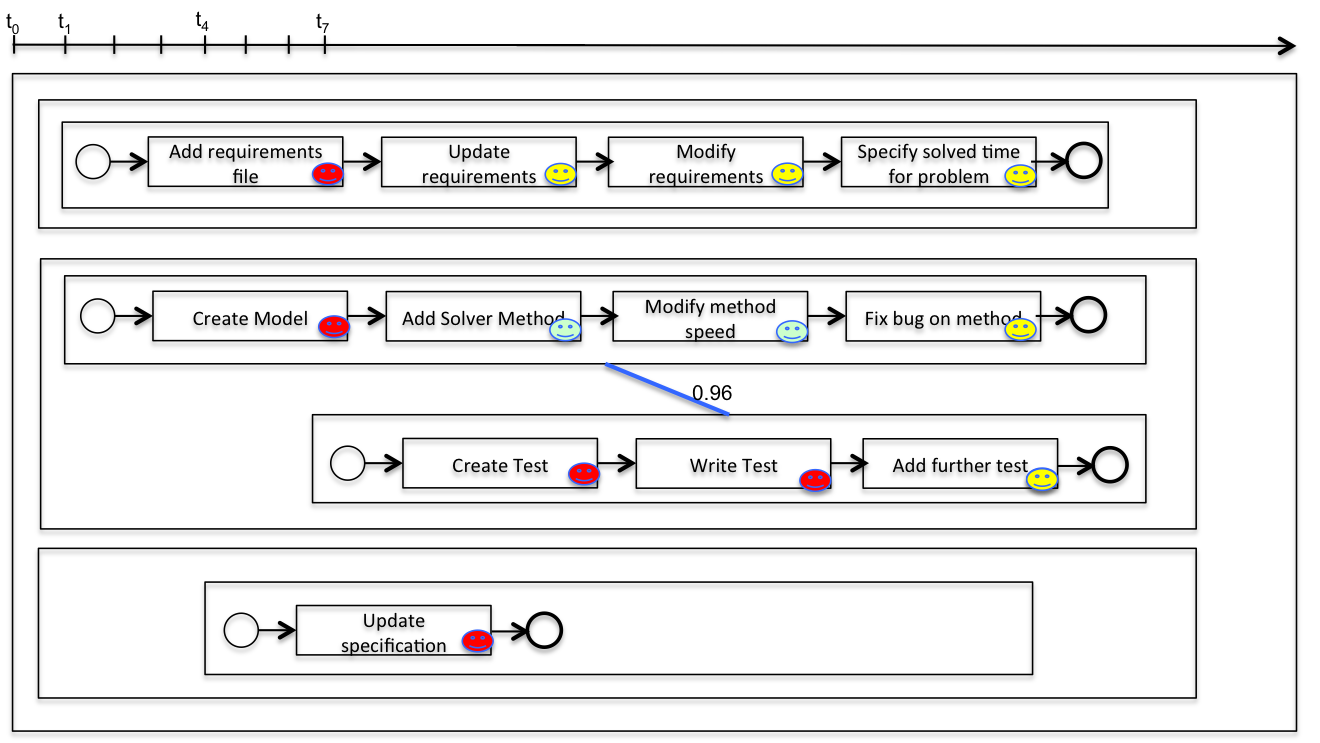
\includegraphics[scale=0.8]{figures/ExampleProposedVisualization}
%\caption{Illustration of the proposed visualization.}
%\label{fig:Containments}
%\end{figure*}
%%}

%ToDo
%Figure with the containments
%Table with the commits (junction of the .xls files. Consider only the amount of change. Express time by $t_i$
%Figure with the containments instanciated with the file processes and the dependencies.


%\subsection{Story Mining}
\label{subsec:story-mining}

%What is story mining and how we use it in our work
Gon\c{c}alves et al.~\cite{Goncalves2011} proposed a story mining approach to extract process elements from stories, i.e. text descriptions written collaboratively by the process participants. A story is a natural way to transmit and share knowledge. Using both natural language (text) and contextual elements (categorization of parts of the story), storytellers can express their experience and viewpoints about the work processes they participate, interact with and/or perceive. Stories have the advantage of reproducing the situations associated with their contexts - the knowledge that is difficult to capture in interviews or mining from Information Systems logs. Since collectively told, a story incorporates a range of perspectives. Business processes instances can also be viewed as stories played by individuals who perform specific roles depending on the circumstances.

Story Mining  \cite{Goncalves2011} receives as input a story freely written by the participants, describing their work in a particular business process. As an output, the \emph{actors} and the process \emph{activities} executed by them are extracted. To illustrate the approach consider the following story. The terms highlighted in {\bf bold} are the actors of the processes and the terms highlighted in {\color{gray} gray} the activities. 

\begin{figure}[!h]
{ \bf The system} {\color{gray} generates an estimating template consisting of the phases, activities and tasks} selected
for the project or project phase. When planning complete projects the estimating is typically done at the activity level, using the
list of tasks in the work breakdown as input to the estimating process. However {\bf estimators} will likely {\color{gray}add an itemized list of system functions and other deliverables}, to facilitate estimating the construction phase. {\bf Multiple estimators} {\color{gray} prepare estimates for each component}, {\color{gray}compare their estimates}, and {\color{gray}arrive at a final estimate} for each item.
  \label{RB}
\end{figure}

A further step that we developed in our approach is the identification of the relationship between the activities, therefore defining the flow.

%\subsection{Project Mining Software Projects}
\label{subsec:proj-mining}

Project mining technique 


\section{Evaluation}
\label{sec:evaluation}

In this section, we show the applicability of our technique to project-oriented business processes and its effectiveness in uncovering work dependencies. With respect to the requirements formulated in \Cref{sec:background}, we evaluate against requirements {R2} and {R3} in \Cref{subsec:quantitative-eval} and against requirement {R1} in \Cref{subsec:qualitative-eval}.

We implemented our techniques as a prototype\footnote{The source code is available at \url{https://github.com/s41m1r/MiningVCS}} and used it on 10 real world software projects with different sizes. The input of our program is a \gls{vcs} log and the output is a set of analysis data with information about the evolution of the artifacts and their dependencies. We report the results in \Cref{table:evaluation-results-new}. The results are listed in increasing order of project size. The parameters $\chi$ and $d$ are the metrics of \emph{degree of co-evolution} and \emph{distance}, respectively. In this example, $\chi > 0.7$ signifies that the co-evolution is high ($\chi^{H}$) and $\chi < 0.3$ that the co-evolution is low ($\chi^{L}$). As previously mentioned, this is a user customizable threshold that can be set by the domain expert. Likewise, the distance is considered low ($d^{L}$) when $d<=2$ and high ($d^{H}$) when $d>2$. The parameter  $\overline{|p_f|}$ and {$max(|p_{f}|)$} are respectively the average and the maximum lengths of the path to the root (i.e. average tree depth of the files). The column {$|A_{evo}|$} shows the average number of activities in the process representing the artifact evolution. Lastly, the columns {$\overline{d}$} and {$max(d)$} report the average and maximum file distance, respectively. Next, we use these data for a quantitative evaluation of the projects.

% Please add the following required packages to your document preamble:
% \usepackage{graphicx}
\begin{table}[t]
\centering
\caption{Evaluation of real world projects. Respectively the thresholds are: $\chi^{L}$ if $\chi < 0.3$,  $\chi^{H}$ if $\chi > 0.7$  low and high degree of co-evolution; $d^{L}$ if $d \leq 2$,  $d^{H}$ if $d > 2$ respectively low and high distance.}
\label{table:evaluation-results-new}
\resizebox{\textwidth}{!}{%
\begin{tabular}{rrrrrrrrrrrrrr}
\
Project                 & \rot{Commits} & \rot{Files} & {$\chi^{H}$} & {$\chi^{L}$} & \begin{tabular}[l]{@{}r@{}}{$(d^{L},\chi^{L})$}\end{tabular} & \begin{tabular}[l]{@{}r@{}}{$(d^{L},\chi^{H})$}\end{tabular} & \begin{tabular}[b]{@{}r@{}}{$(d^{H},\chi^{L},)$}\end{tabular} & \begin{tabular}[l]{@{}r@{}}{$(d^{H},\chi^{H})$}\end{tabular} & \rot{$\overline{|p_f|}$} & \rot{$max(|p_{f}|)$} & \rot{$|A_{evo}|$} & \rot{$\overline{d}$} & \rot{$max(d)$} \\ \midrule
%smsr                    & 21        & 6         & 22                   & 6                  & 0                          & 9                            & 6                       & 13                        & 2.71             & 5             & 1.82                    & 1.43                & 6                  \\
mwaligner  & 21      & 9     & 37                   & 7                 & 6                               & 30                                 & 1                                          & 7                                             & 1.11              & 2           & 2.40         & 0.94                 & 3                 \\
Biglist                 & 202     & 15    & 22                   & 90                & 31                              & 18                                 & 59                                         & 4                                             & 1.47              & 3            & 2.76         & 1.20                 & 5                 \\
camundaRD & 11      & 15    & 74                   & 26                & 0                               & 25                                 & 26                                         & 49                                            & 2.18              & 4            & 2.05         & 2.03                 & 7                 \\
graphql                 & 256     & 30    & 89                   & 357               & 121                             & 89                                 & 236                                        & 0                                             & 1.40              & 2            & 3.18         & 1.11                 & 4                 \\
jgitcookbook            & 135     & 89    & 773                  & 2866              & 505                             & 289                                & 2361                                       & 484                                           & 6.93              & 8            & 1.33         & 2.68                 & 14                \\
mysqlpython             & 749     & 168   & 2288                 & 11571             & 742                             & 591                                & 10829                                      & 1697                                          & 2.59              & 7            & 1.65         & 2.52                 & 11                \\
gantt                   & 23      & 228   & 7006                 & 14343             & 386                             & 3480                               & 13957                                      & 3526                                          & 3.30              & 4            & 1.71         & 2.16                 & 7                 \\
facebookjavasdk         & 38      & 293   & 16478                & 26092             & 2017                            & 16311                              & 24075                                      & 167                                           & 6.21              & 8            & 4.78         & 5.58                 & 13                \\
caret                   & 864     & 432   & 15366                & 60874             & 9538                            & 14785                              & 51336                                      & 581                                           & 3.01              & 4            & 3.15         & 1.60                 & 7                 \\
operationcode           & 1114    & 1053  & 84024                & 444605            & 2291                            & 5537                               & 442314                                     & 78487                                         & 4.27              & 8            & 2.01         & 4.85                 & 15               \\
\end{tabular}%
}
\end{table}
%\vspace*{1cm} 

%\subsection{Prototypical Implementation}
\label{subsec:prototype}


%
%The first step of the approach is the preprocess of the VCS log received as input. The main goal of this phase is generate a set of events and store them into a database. Second, we obtain different views on the stored events. In particular, we are interested in observing
%\begin{inparaenum}[\itshape i)]
%	\item all the commits that affected the files over time;
%	\item the amount of change brought by the commits to the files; and
%	\item the users who issued such commits.
%\end{inparaenum}
%The third phase is responsible for considering the different perspectives defined by the project manager and through the generated views extract the necessary knowledge. The last phase is responsible for providing the visualization combining the different perspectives considered. The following sections detail each of the phases.

We implemented our technique as a prototype\footnote{\url{https://github.com/s41m1r/MiningVCS.git}}. The input of our program is a \gls{vcs} log and the output is a set of analysis data with information about the evolution of the artifacts and their dependencies. 
%%Next we show the implementation details of \Cref{algorithm:all}.
%
%
%
%%\subsubsection{Preprocess VCS Logs.}
%As a first step (cf.~\Cref{algorithm:all}) we need to preprocess the input in order to extract events. Events in \gls{vcs} have multiple dimensions and relations among one another. Therefore, the natural way of capturing them is through a relational data model. This model serves at structuring the raw data and persisting the results after first step of \Cref{algorithm:all}. \Cref{fig:data-model} outlines the main entities in a \gls{vcs} and the relationships of our interest. The result the first step of \Cref{algorithm:all} is the correct population of the a database with the set of the extracted events, stored according to the relational schema. 
%
%\begin{figure}[]
%	\centering
%	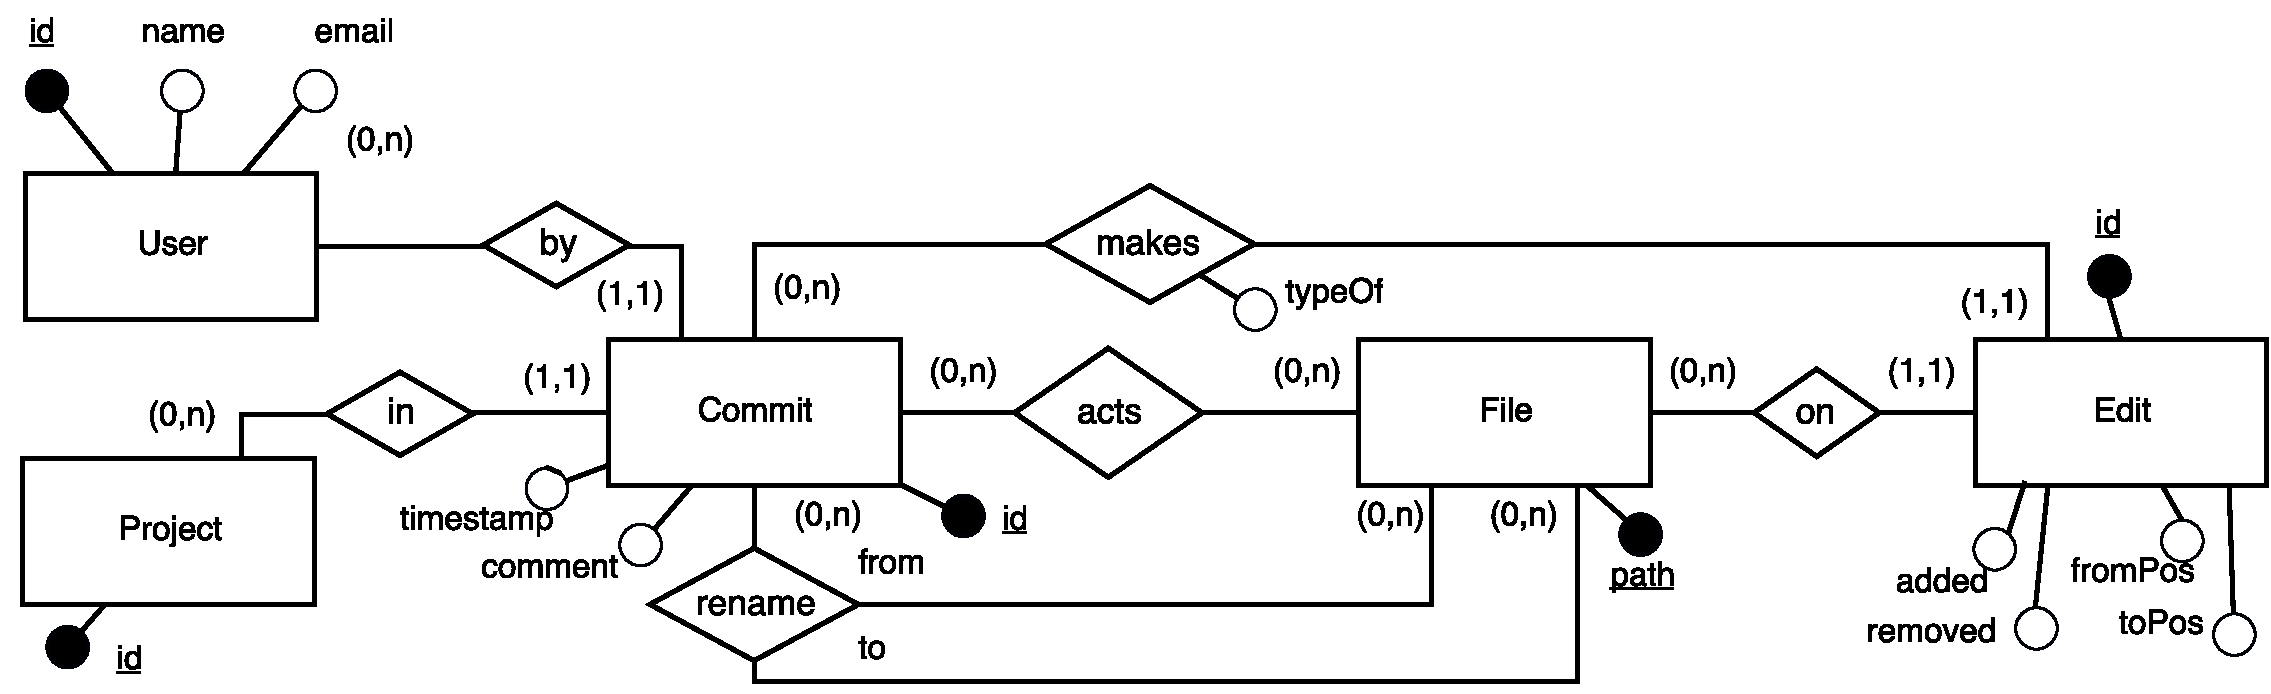
\includegraphics[width=0.9\linewidth]{figures/CommitLogER}
%	\caption{Relational schema of a software project}
%	\label{fig:data-model}
%\end{figure}
%
%%\subsubsection{Obtain View on Project.}
%
%The step~\ref{algorithm:all} makes queries over the event set in order to retrieve aggregated views from them. This is simply done by defining queries on the database and export collect their results (e.g., in a CSV file). Step~\ref{step:contaiments} consists in recreating the file structure. This is implemented by reverse engineering the directory structure from the \texttt{path} attribute of the entity \texttt{File} that is present in the output of the query. Next, we actuate step~\ref{step:evolution} by implementing \Cref{algorithm:compute-evolution} that computes the artifact evolutions. This algorithm takes as input the set of views calculated previously and outputs \begin{inparaenum}[\itshape i)]
%	\item and a set of \emph{file stories} that report the amount of change, time and comments of the file history, and
%	\item a set process that describe the evolution of every artifact obtained by story mining~\cite{Goncalves2011} the file stories.
%\end{inparaenum} Finally, for step~\ref{step:dependencies} we implement \Cref{algorithm:compute-dependencies}. This algorithm takes as input the aggregated views obtained previously and two parameters: a comparison function and a threshold. We use the Pearson correlation $\rho$ and let the domain expert set the threshold $\delta$ to filter the strength of the dependencies. An important step before 


%One example of query that outputs a view of the daily changes of the artifact \texttt{model.java} is shown in \Cref{lst:query}. 

%\begin{center}
%\begin{lstlisting}[
%language=SQL,
%showspaces=false,
%float=ht,
%xleftmargin=4em,
%aboveskip=6pt,
%belowskip=0cm,
%belowcaptionskip=0cm,
%basicstyle=\ttfamily\scriptsize,
%showstringspaces=false,
%commentstyle=\color{gray},
%mathescape=true,
%caption={SQL query to obtain the artifact history for a given artifact, aggregated on a day level},captionpos=b, label={lst:query}
%]
%SELECT CONCAT(Commit.comment,$\S$) as Comments, 
%	DATE(Commit.timeStamp) as Date, 
%	sum(linesAdded+linesRemoved) as Change, 
%	CONCAT(User.name, '$\S$') as Users
%FROM File, Edit, acts,Commit,User 
%WHERE File.path = 'model.txt' 
%	AND Edit.commit_id = Commit.id 
%	AND Edit.file_path = File.path
%	AND User.id = Commit.user_id
%	AND acts.file_path = File.path 
%	AND acts.commit_id = Commit.id
%GROUP BY Date
%ORDER By Date ASC
%\end{lstlisting}
%\end{center}
%
%\Cref{table:analysis-data} depicts a view obtained with the query in \Cref{lst:query} on the project shown in \Cref{subsec:scenario}. The data is aggregated by day. String values are concatenated together with the symbol '$\S$'.
%
%\input{tables/analysis-data}

%\subsubsection{Analyze project data.}

%The input of this phase is a collection resulting from querying all the artifact histories from the data store. At this point the data is ready to be analyzed. 
%In this step analyses on the view extracted are performed. There are a number of different analyses that can be applied directly to the \emph{aggregate events}, e.g. checking whether project participants have been working on the assigned tasks ("Are they working in the artifacts they should/?") or there has rather been disorganization in regards. In this work, we focus on analyzes related to the artifacts, i.e. how they evolve over time, how they are organized and how are the dependencies among them. Therefore, in this section we focus on extracting the \emph{containments}, \emph{dependencies} and \emph{artifact evolution} elements.
%
%Analyzing the \emph{Parent} relation, the set $C$ of containments for our scenario of use is: $C = \{f_1, f_3, f_4, f_6, f_9, f_{10}\}$. 
%
%\begin{table}[t]
%%	\centering
%	\caption{Time series similarity among the six artifacts}
%	\label{table:time-series-all}
%	\begin{subtable}{.45\linewidth}
%		\input{tables/times-series}
%	\end{subtable}
%	\begin{subtable}{.45\linewidth}
%		\input{tables/correlations}
%	\end{subtable}
%\end{table}
%
%To compute the dependencies, we analyzed the time series depicted in \Cref{table:time-series} computing the correlations pairwise. Considering that the project manger specified a threshold of 0.7, we found the dependencies: \{(${f_7}$,${f_5}$), (${f_7}$,${f_8}$), (${f_2}$,${f_5}$), (${f_2}$,${f_{12}}$), (${f_5}$,${f_{12}}$)\}.
%
%The last step in this phase is the computation of the artifacts evolution. For all 6 artifacts a story containing the comments observed in the aggregate events for that artifact was generated. In the end, six stories were created and for each of them our approach for artifact mining was applied. 

\subsection{Quantitative Evaluation}
\label{subsec:quantitative-eval}

Here we address requirements R2 and R3. First, we compute project profiles. These profiles show the distribution of work-related dependencies in a project. Second, we evaluate whether the work on files can be predicted.

Before assessing project profiles, we make the following consideration. Our metrics define four classes:
\begin{inparaenum}[\itshape i)]
	\item low distance low co-evolution;
	\item high distance low co-evolution;
	\item low distance high co-evolution;
	\item high distance high co-evolution.
\end{inparaenum} \Cref{fig:pairs-on-space} helps clarifying these four classes. In fact, except for values of distance equal to 0, it is possible to see how the density of file pairs is higher when the distance is low. This is a normal situation in project where highly related files are stored closely to each other in the file system. Conversely, the dots on the top right of the plot mark files which are very distant to each other but still highly correlated. These can be, for instance, logical dependencies that can happen because of bad modularization of the project.

Hidden work dependencies belong to the last mentioned case, i.e. files are distant in the file tree but they have similar time series. According to this consideration we computed the project profiles in \Cref{fig:project-analysis}. We observe three types of processes. First, several projects have hardly any hidden work dependencies. Second, several have a moderate degree between 10\% and 20\%. Third, the project \textit{Biglist} has a high share of hidden dependencies. This hints at the possibility for better organizing the project according to good modularization best practices. That means, the project can be restructured in a way to reduce the unwanted side-effect the work on one file produces on other files.
%\input{tables/project-assessment}


%\begin{figure}
%\centering
%
\includegraphics[width=0.3\linewidth]{figures/assessment-diagram}
%\caption{Project assessment diagram}
%\label{fig:assessment-diagram}
%\end{figure}
\begin{figure}[t]
	\begin{subfigure}[b]{.51\textwidth}
		\centering
		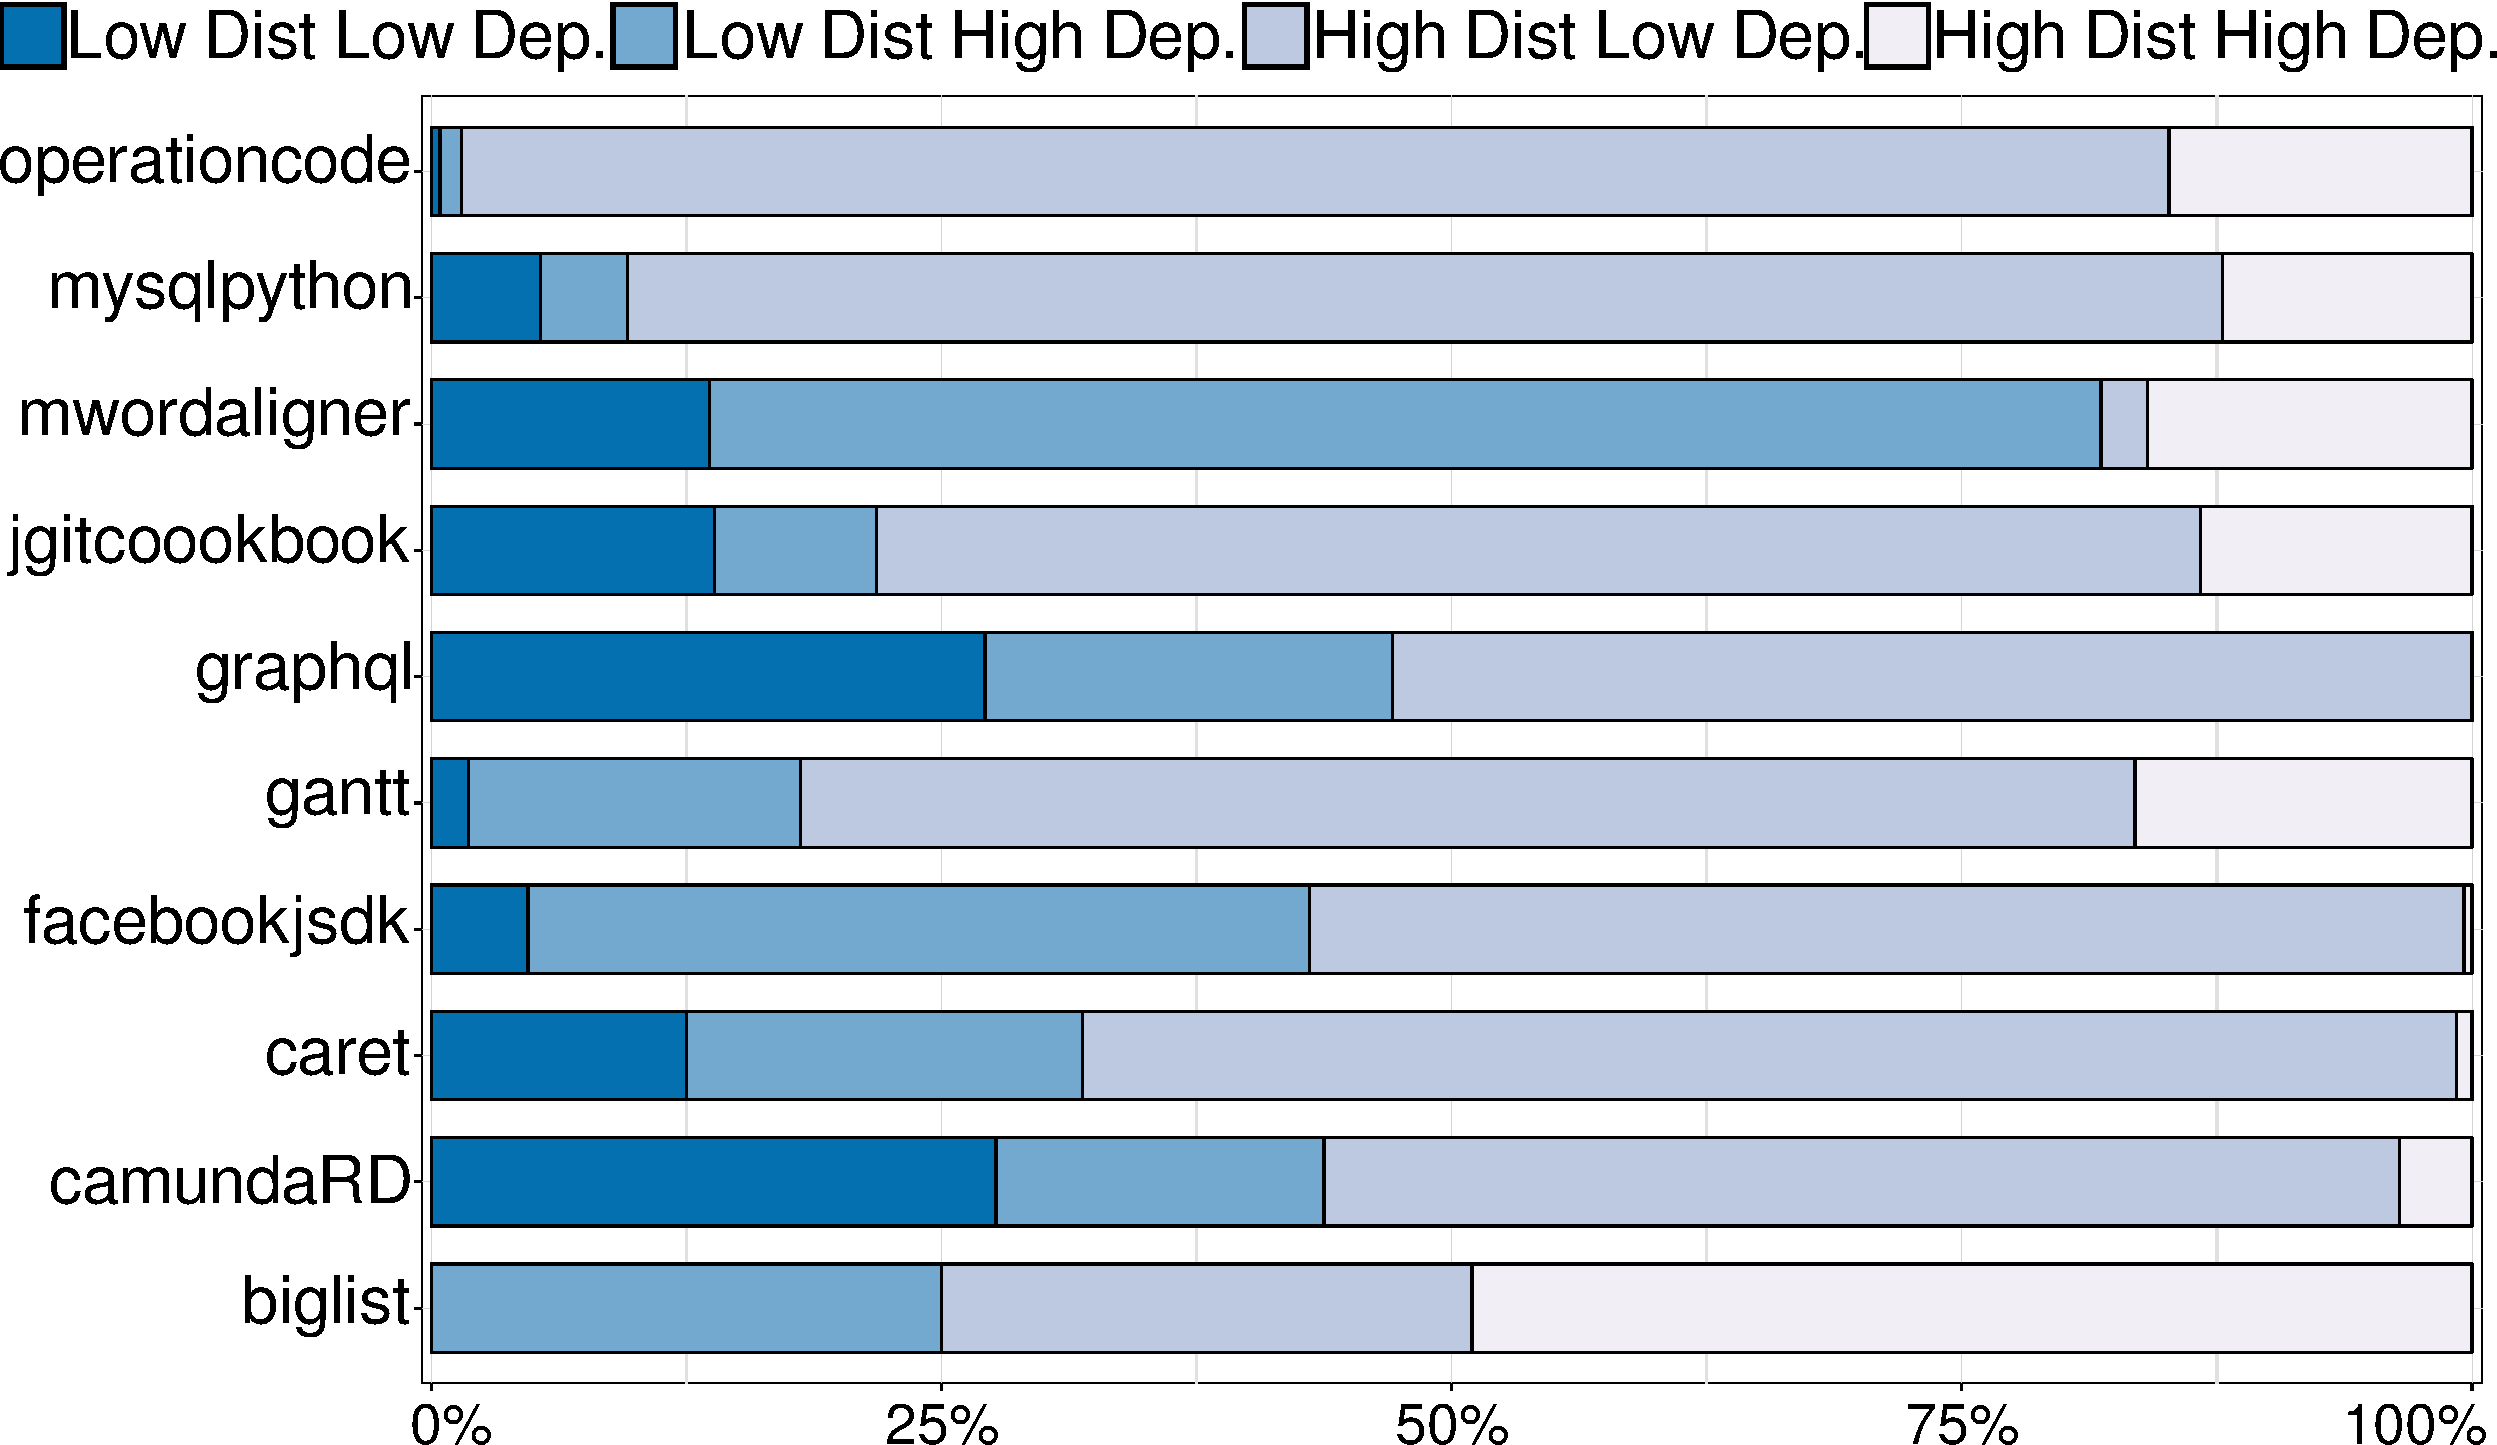
\includegraphics[width=.98\linewidth]{bpm2017/figures/Project-Analysis-Barchart-crop.pdf}
		\caption{Evaluation on real projects}
		\label{fig:project-analysis}
	\end{subfigure}~
	\begin{subfigure}[b]{.47\textwidth}
		\centering
		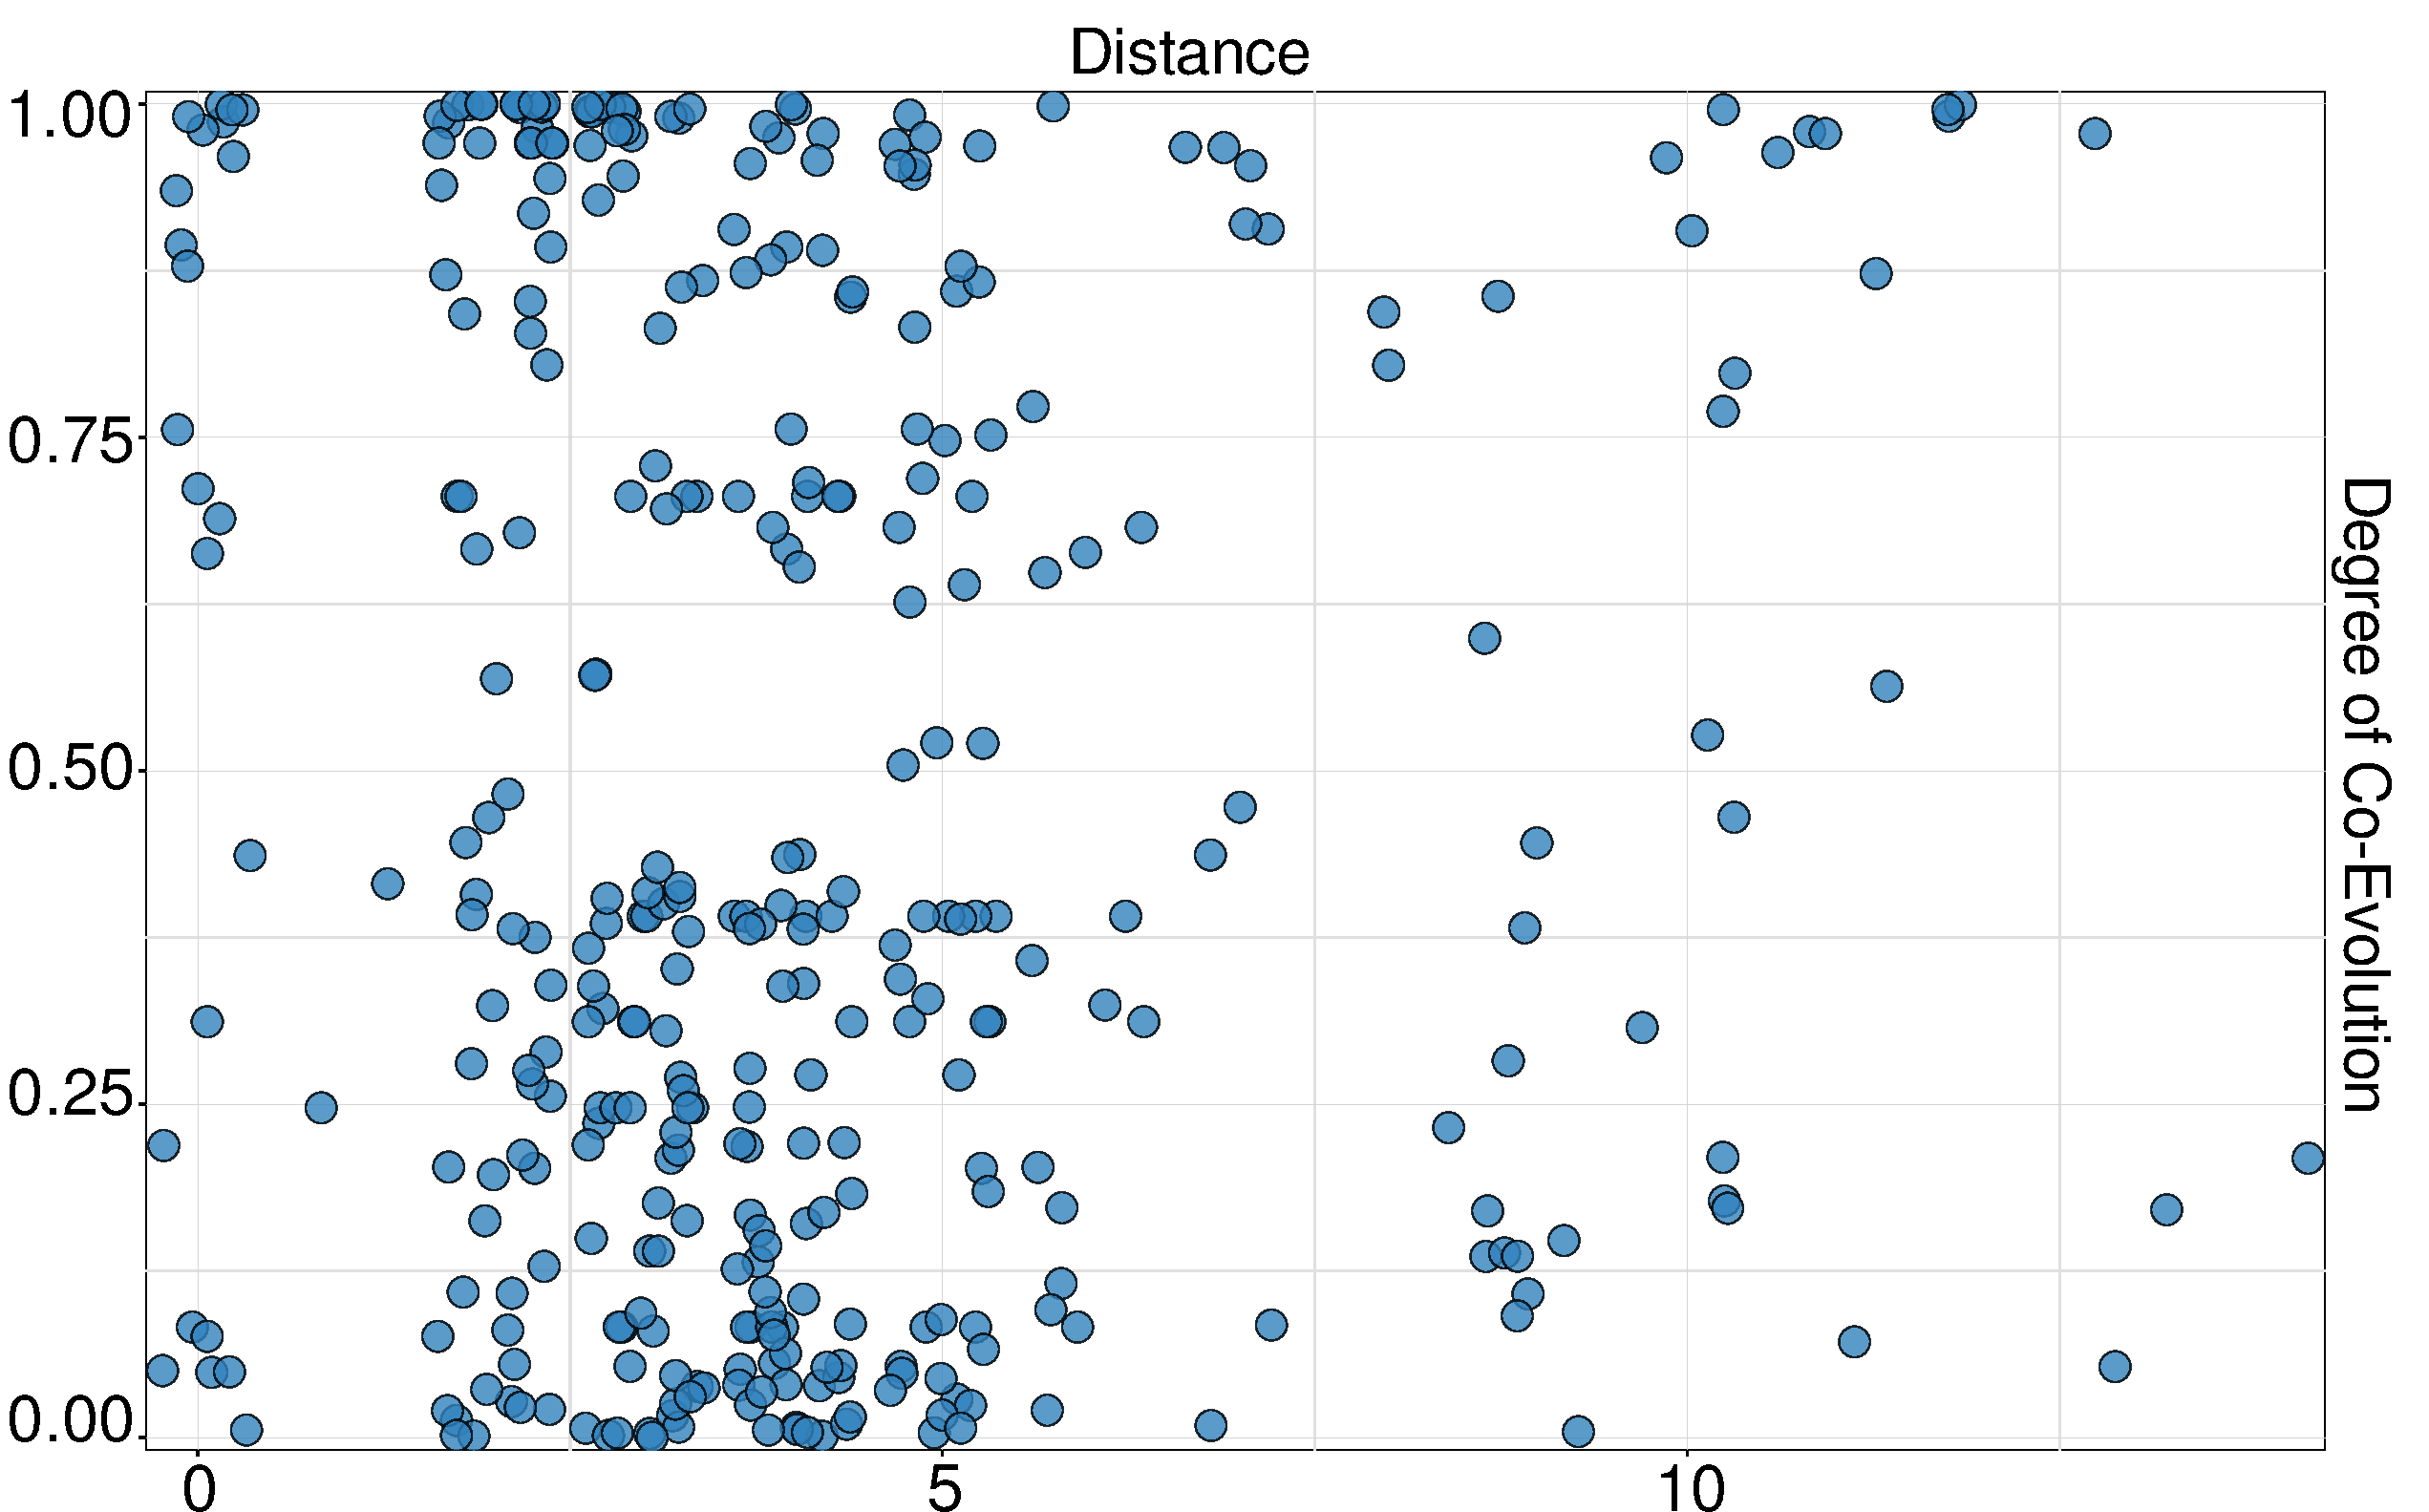
\includegraphics[width=.98\linewidth]{bpm2017/figures/Co-EvolutionVSDistance-OneColor.pdf}
		\caption{Distribution of pairs on real projects}
		\label{fig:pairs-on-space}
	\end{subfigure}
%	\vspace*{-.5cm}
	\caption{Characterization of the evaluated software projects}
\end{figure}
Next, we evaluate whether the work on files can be predicted. Zipf's law is typically used in corpus analysis and states that the \emph{frequency} of usage of any word is inversely proportional to its \emph{rank} in the frequency table. This approach has already been applied to software projects for understanding whether the assignment of developers to tasks in a software project could be predicted~\cite{Canfora2006}. Here, we focus on understanding whether the Zipf's law holds true also for work dependencies within a project. 

To this end, we selected one big and one small project from \Cref{table:evaluation-results-new}, namely \emph{Biglist} and \emph{Caret}. Biglist is a small project on a list of strings which are known to cause issues when used as user-input data. Caret is a big project consisting in the development of a sublime text editor for Chrome OS.
We collected how frequently were the artifacts worked on to generate a ranking. \Cref{fig:zipf-graph} depicts the corresponding charts and the fitted Zipf distribution. We notice that both projects present a similar distribution of values. This holds also for the other projects analyzed. In particular, Zipf's law is valid for the most frequently changed files. Afterwards, the distribution drops because of files not being worked anymore but still being part of the project.
%In pure software development projects, the tail can hint at some dead code and the need for maintenance.

\begin{figure}[t]
%	\centering
	\begin{subfigure}{.5\textwidth}
		\centering
		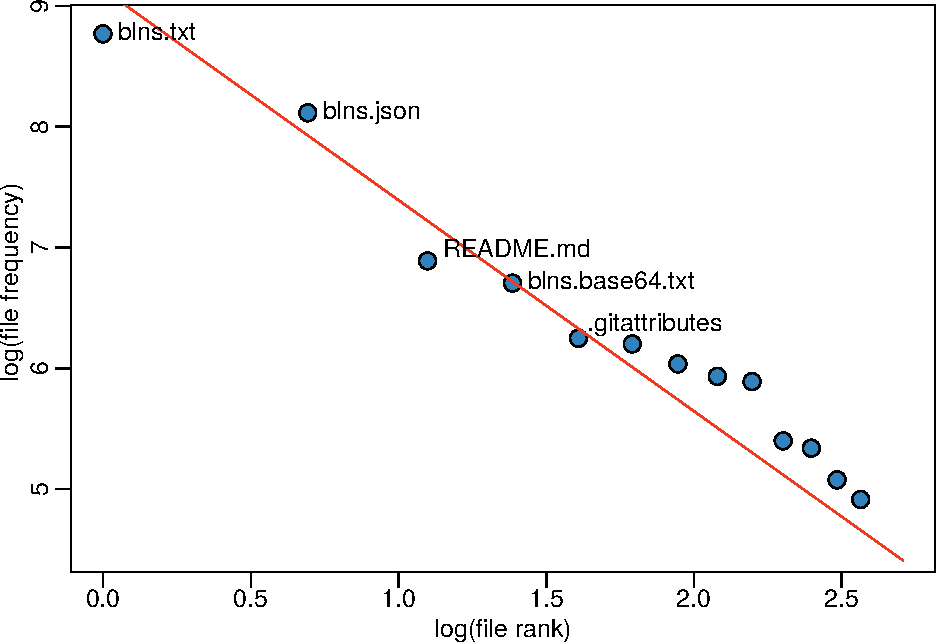
\includegraphics[width=\linewidth]{bpm2017/figures/biglist-new-crop}
		\caption{Biglist project}
		\label{fig:biglist}
	\end{subfigure}%
	\begin{subfigure}{.5\textwidth}
		\centering
		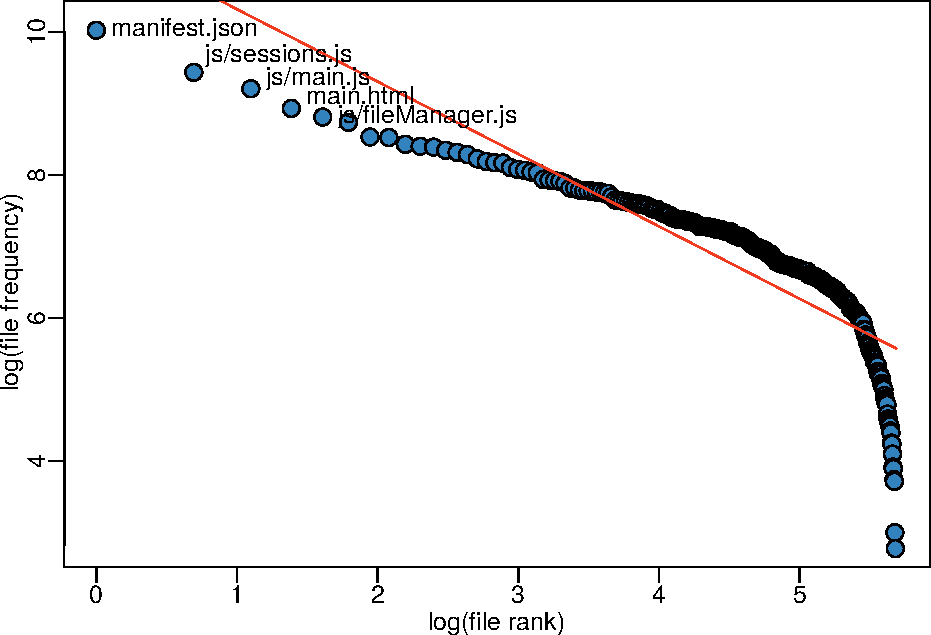
\includegraphics[width=\linewidth]{bpm2017/figures/caret-new-crop}
		\caption{Caret project}
		\label{fig:caret}
	\end{subfigure}
%	\vspace*{-.3cm}
	\caption{Zipf distribution of the worked files}
	\label{fig:zipf-graph}
\end{figure}
%\vspace*{-.2cm}

\section{Discussion}
\label{subsec:qualitative-eval}

In this section, we address requirement R1 by showing insights on the work history of files that are related. To this end we focused on the project \emph{smsr}, which has 21 commits over a time span of ten days.

%\todo[inline]{an example where it succeds:}
%\subsubsection{Example of work dependencies.}
%\subsubsection{Example of correct discovery.}
%\label{subsub:example}
Let us consider an example where our technique proves helpful. Our technique finds 6 highly related pairs, as shown in \Cref{table:evaluation-results-new}. We excluded files that have a functional dependencies, e.g. interface-class relations, where a change in the interface trivially brings change in the class. Thus, we were able to select the files \texttt{smsr/running example/Requirements/requirements.txt} and \texttt{smsr/running example/Software/model.java}, having $\chi=0.7$ and $d=4$. Moreover, by observing the content we verified that they do not have functional dependencies. Therefore, these two files are work dependent.
\Cref{fig:evaluated-processes} shows the extracted processes after mining their stories. Interestingly, the two processes do not share any activity because they were never changed together in the same commit.
%Literature approaches that leverage on network analysis can not uncover these type of dependencies, which are instead visible by the time series analysis.

\begin{figure}[t]
	\begin{subfigure}[t]{\textwidth}
		\centering
		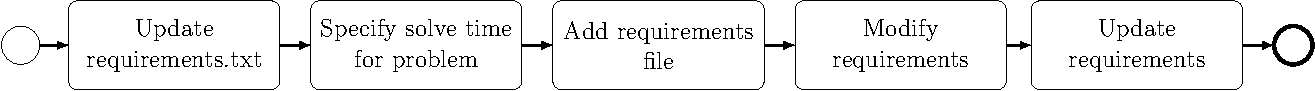
\includegraphics[width=.9\linewidth]{bpm2017/figures/six-processes/requirementsTxtProcess}
		\caption{Evolution of file \texttt{requirements.txt}}
		\label{subfig:requirements-file-process}
	\end{subfigure}
	\begin{subfigure}[ht]{\textwidth}
		\centering
		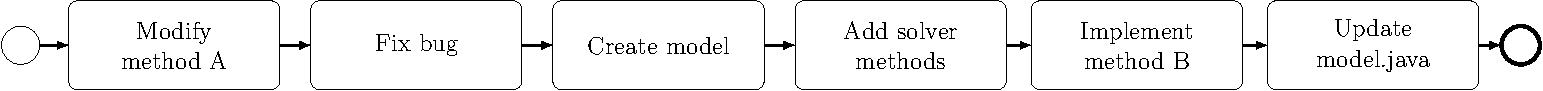
\includegraphics[width=.9\linewidth]{bpm2017/figures/six-processes/modelProcess.pdf}
		\caption{Evolution of file \texttt{model.java}}
		\label{subfig:model-file-process}
	\end{subfigure}
	\caption{Processes of two work-dependent files}
	\label{fig:evaluated-processes}
\end{figure}
%\todo[inline]{An example where it fails for some specific reason:}
%\subsubsection{Example of challenge.}

Our technique can fail under some circumstances. Consider the example above. We know that the files \texttt{requirements.txt} and \texttt{model.java} are work dependent. Let us now assume that the assumption of \emph{regular commits} in the \gls{vcs} does not hold. Nevertheless, we know that there is the following work pattern: \emph{at irregular times, one change in the requirements produces 2 changes of work that must be implemented in model in the next day}. In a short time window of 4 days, the time series would be $X_{req} = (1,0,1,0)$, $X_{model} = (0,2,0,2)$ and their correlation is $\sigma(f_{req},f_{model}) = -1$. Hence, they would score a high degree of co-evolution $\chi=1$. However, if we double the time window  and observe only another pattern the correlation would change. We get $X_{req} = (1,0,1,0,0,1,0,0)$, $X_{model} = (0,2,0,2,0,0,2,0)$ which score a $\sigma(f_{req},f_{model}) = -0.66$, $\chi=0.66$ and therefore not a high value of correlation.
%In these cases, approached that mine patterns of changes would outperform our approach.

These results show that our technique helps uncovering work dependencies that are not captured by existing approaches in literature which leverage on social network analysis~\cite{Zimmermann2008,Weicheng2013}. On the other hand, our technique is currently not yet able to retrieve dependencies with delay. We plan to address this challenge by using moving-average time series models. 

%\subsection{Discussion.}

\Cref{subsub:example} shows that time series analysis can help uncovering work dependencies that are not captured by existing approaches in literature which leverage on social network analysis~\cite{Zimmermann2008,Weicheng2013}. On the other hand, our technique is currently not yet able to retrieve dependencies with delay. We plan to address this challenge by using moving-average time series models.
%However, we argue that on the long run, under the assumption that \gls{vcs} is used in the everyday work, the technique can be useful to further 


\section{Conclusion}
\label{sec:bpm2017conclusion}

In this paper, we addressed the problem of uncovering hidden work dependencies from \gls{vcs} logs. The main goal was to provide project managers with knowledge about the artifacts co-evolution in the project. Three perspectives of analysis were considered, evolution of the artifacts over time, dependencies among them and structural organization of the project.Our approach works under the assumptions that repositories reflect the hierarchical structure of the project, project participants commit their work regularly during active working
times and they provide informative comments for the changes done. The approach was implemented as a prototype. A scenario of use was provided showing how the approach can be applied and providing some discussions. We also evaluated our approach in real-world data from open source projects showing the potential of the approach.

In future work, we will improve our evaluation varying for instance the time window, the dependency threshold and consider a study case with project managers. We plan to investigate other types of dependencies between artifacts. Specifically, we are interested in a semantic analysis of the work performed in both artifacts, considering for instance some similarity measures. We also aim to improve the visualization to consider other knowledge extracted, for instance the type of change performed in the aggregate events could be shown associated to the activities in the artifact process.




\chapter{Software development process evaluation based on integration of stakeholder perceptions and software development tool logs data}

\todo[inline]{Damjan work}

New important theoretical development for SDM evaluation - complementing stakeholder perceptions with data about actual execution of the software development process.

\section{What are the perceptions of developers and managers about the work?}

\section{What has been done in the past?}

\section{What we propose}

\section{Evaluation}

\section{Discussion}


\chapter{The Conversational Structure of Problem-Solution Co-Evolution}

\section{First section}



\chapter{Discussion}
\label{ch8-discussion}



\chapter{Conclusion}
\label{ch9-conclusion}

This chapter summarizes the main contributions of the dissertation. \Cref{sec:summary-of-results} lists the results. \Cref{sec:8-discussion} discusses in more detail their impact. \Cref{sec:8-future} outlines future research. 

\section{Summary of Results}
\label{sec:summary-of-results}

This doctoral thesis aims at bridging the gap between automatic analysis of software development data and process mining. It provides analyses techniques that help learning specific characteristics of the software process from its trace data. This thesis makes the following contributions.

\begin{itemize}
	
	\item \textbf{Conceptualization of project-oriented business processes.} Processes have been seen so far as repeatable endeavors. However, there are processes which are not repeated exactly in the same way twice. This is the case with project-oriented business processes. Such processes, are conducted as projects, in that they are usually planned a priori and run under limited resources. 
	
	\item \textbf{Visualization.} This thesis provides more suitable visualization techniques that help understanding the work process that lies behind software development. More specifically, we presented different possible visualizations to better represent each of the four perspectives of a business process. By mining a GANTT chart, artifact A1 gives insights into the time perspective. By uncovering the hidden co-evolution of software components such a files, artifact A2 shows explicitly the variation of different cases. By mining roles, artifact A3 visualizes de-facto profiles for each developer. By mining activities and their order, artifact A4 gives insights into the control-flow. 
	
	\item \textbf{Extension of the scope of process mining.} Process mining techniques rely on structured data. Typically these data come from \gls{pais}. The artifacts constructed in this thesis handle data which were not generated by \gls{pais}. Thus, they provide a use case for extending the scope of process mining. 
	
	\item \textbf{Datasets for further research.} During the course of this research a number of datasets have been generated. The artifacts produced by this dissertation provide preprocessed datasets and algorithms that can be used for a variety of analyses on the software process. These datasets are available for further use by researchers who want to replicate these studies or pursue different goals using similar concepts to the ones presented in this thesis. 
	
\end{itemize}


\section{Research Questions Revisited} 
\label{sec:8-discussion}

This section revisits the research questions introduced in \Cref{sec:problem-definition} and discusses how this thesis addressed each of them. More specifically the general question this thesis aims at answering is the following.
\begin{question}{Main Research Question}
	\textbf{RQ}: \emph{How can we make use of project event data to gather insights about the software development process that are informative to managers?}\\
	 
	
	
	Trace data can be exploited to obtain a more realistic evaluation of the current state of the software project. Among the articles presented in this thesis, Article 5 presents a case-study where the importance of trace data is highlighted. While there have been many approaches that try to assess the software process (e.g., \citep{DBLP:journals/bise/VavpoticRH20,hovelja2015exploring,atkinson1999project}) with various methods, there was no approach that exploits both \emph{subjective} data gathered from questionnaire and \emph{objective} data from software development. Thus, the case study presented in Article 5 implements a one-of-a-kind data-driven computationally-intensive approach \citep{DBLP:journals/isr/BerenteSS19} to gather insights the software process. 
	In particular, key difficulties in the performance of the \gls{sdlc} of the analysed company were discovered. These results were only possible thanks to the combination of the subjective views of process participants and the analyses of the event logs. The latter served to confirm or dis-confirm the importance of certain \gls{sdm} elements with regards to performance.
	
\end{question}

This question is addressed in detail by applying mining techniques to event data from software projects. In particular, this thesis applies the four-perspectives view on processes defined in the work of \cite{DBLP:books/sp/Aalst16}. Consequently the main research question is divided into four sub-questions, each addressing one specific perspective.  In the following, each research sub-question \textbf{RQ1} – \textbf{RQ4} is discussed.\\


\begin{question}{Mining the Time Perspective}
\textbf{RQ1.} \emph{How can we use project event data to extract information about the \textbf{temporal} perspective of activities?}\\


RQ1 is addressed by Artifact A1. The context of in which this artifact was developed is that of large engineering software development projects. These projects need to be monitored in detail to understand what work was done \emph{when}. This is particularly relevant when it comes to checking compliance with rules and regulations such as ISO/IEC/IEEE 15288 \citep{international2015iso}. A typical problem of these processes is coordination as it is difficult to tract the actual course of work, even if the data is recorded in \glsfirst{vcs}. Artifact A1 addresses this problem by defining a mining technique that is able to handle data from \gls{vcs}. Furthermore, Artifact A1 provides a time-based visualisation that allows to cluster together periods of work that were done in the different parts of the software directory structure. The models are rendered as Gantt charts in order to best address project managers, as these are directly comparable to projects plans. The artifact was implemented as a prototype, which gives the user both aggregated information in the form of Gantt chart activities and detailed information on the single events. This improves the information gives by similar process mining software such as the Dotted Chart Miner \citep{Song2007}. Moreover, no existing process mining tool gives Gantt chart support.
\end{question}



\begin{question}{Mining the Case Perspective}
	\textbf{RQ2.} \emph{How can we use project event data to extract information about the \textbf{case} perspective?}\\
	
	
	Mining the case perspective in the software development process signifies to uncover characteristics of cases (i.e., the different ways in which files are worked on). This is difficult because work in such process is fragmented between different modules which are developed concurrently. Prior contributions in the areas of \glsfirst{msr} and process mining have proposed a plethora of techniques that analyse and visualize the current state of a software as a product. Surprisingly, a process view (i.e., what type of work is conducted at different stages and what are activity dependencies) was still lacking. Artifact A2 addresses such gap via a technique that can extract the evolution of each file as a time series (i.e., it provides a characterisation of the changes of the file as a process case) and it further classifies the type of work (i.e., the process activities) based on \gls{nlp} techniques. Efficacy of the devised Artifact A2 is demonstrated by applying the technique on various open-source projects. 
\end{question}





\begin{question}{Mining the Organisational Perspective}
	\textbf{RQ3.} \emph{How can we use project event data to extract information about the \textbf{organizational} perspective?}\\
	
	
	Collaboration in business processes and projects requires a division of responsibilities among the participants who are then expected to perform specific tasks based on their role in the organisation. However, in practice process participants are free to perform software developments tasks. The type and amount of tasks that are done by the participants define a so-called \emph{profile}. Profiles are \emph{de-facto} roles may differ from the assigned roles by the project manager. Artifact A4 defines a technique to collect participants' profiles from \gls{vcs} logs and classify them into classes of roles. It does so via two approaches, which are then compared. The first approach finds classes of users by applying k-means clustering to users based on attributes calculated for them. The classes identified by the clustering are then used to build a decision tree classification model. The second approach classifies individual commits based on commit messages and file types. The distribution of commit types is used for creating a decision tree classification model. The two approaches are implemented and tested against three real datasets, one from academia and two from industry. Our classification covers 86\% percent of the total commits. The results are evaluated with actual role information that was manually collected from the teams responsible for the analysed repositories. In practice, the developed artifact helps the project manager to better understand the actual type of work that is required in developing a specific software product.
\end{question}

 


\begin{question}{Mining the Control-Flow Perspective}
	\textbf{RQ4.} \emph{How can we use project event data to extract information about the \textbf{control-flow} perspective?}\\
	 
	
	RQ4 is addressed by Artifact A4. This artifact is developed with the assumption that the complexity of software development process is hard to be discovered as a single process model. In fact, existing models of the \gls{sdlc} always remain at a high level of abstraction and never specify exactly the low-level activities that constitute the different phases of software development. Moreover, many \glspl{sdlc} models assume that certain activities (or phases) of software development happen in a specific order and never overlap. An exception to this is the so-called \glsfirst{rup} model, which acknowledges that different phases of the development can be done concurrently. However, the \gls{rup} has only been a theoretical model so far and no tools were developed to mine such model from data. Artifact A4 was developed to fulfil this goal. It uses data from \gls{vcs} to analyse to mine the activity types of which the development process consists. The artifact is implemented as a prototype in Java and its outputs evaluated in terms of effectiveness against existing real-world repositories from GitHub. As a result, various patterns of software development were found and visualized according the \gls{rup} model. In this way, it was possible to understand the how the work transitioned among the different phases (i.e., the control-flow) of software development. 
\end{question}

\section{Future Research and Concluding Remarks}
\label{sec:8-future}

There are several ways in which current research can be improved. 

\begin{itemize}
	\item {\bfseries Develop more advanced visualisation techniques.}
	Visualisation is key to process understanding \citep{DBLP:journals/corr/abs-2202-07941}. An interesting follow-up of this research would be to provide an integrated visualization that brings all four perspectives together in a way that would be beneficial to the managers. This would give a clear bigger picture of the impact of each perspective and let the manager decide which of these to prioritize when it comes to improvement. Therefore, the manager has more control over the project and capacity to react to potential issues. 
	
	\item{\bfseries User studies.}
	Qualitative analyses of the impact of the proposed artifacts in an industrial context. User studies should be conducted for each of the artifacts in order to investigate their perceived usefulness and ease of use \citep{DBLP:journals/misq/VenkateshMDD03}. With this feedback the already developed artifacts can be improved. 
	
	\item{\bfseries Integrate different datasets.}
	Another point concerns the data used for the analysis. This thesis used data from one source at a time such \gls{vcs} or Jira. However, data present in these systems only store part of the overall end-to-end software development methodology. Integrating data from diverse systems \citep{DBLP:conf/icse/TrautschTHLG20}, such as project planning systems, emails, documents, etc, would enable for learning more about the overarching software process (e.g., the end-to-end process from idea-inception to software-product release). This, in turn, would open up chances for process redesign or innovation. 
	
	\item{\bfseries Coordination studies.}
	Coordination is an important topic when it comes to software development. Future work shall investigate how control happens in \gls{oss}. Especially, it should aim at shedding light on the how collaborative processes unfold when several users are free to join existing software projects as contributors. \Gls{floss} projects have been brought as an example of innovative ways of self-organizing \citep{DBLP:journals/mansci/KroghH06,DBLP:journals/misq/HowisonC14}. Works in literature have emphasized iterations (\citealp{Berente2005,Berente2007}), self-organization \citep{DBLP:journals/infsof/CrowstonLWEH07,DBLP:journals/jss/HodaM16} and free-speech \citep{DBLP:conf/chiir/ThomasCMCM18,Gibson2019}. However, it has been shown that control mechanisms (be there social or institutional) are present in the area \citep{Lindberg2016}. In particular, online collaborative work that generates knowledge goes through ``negotiation'' actions which ``pull'' the trajectory and shape its movement in the feature space \citep{Arazy2020}. Therefore, it remains under-explored to what extent \gls{oss} is institutionalized and what are its similarities to corporate bureaucracy.
	
	A possible way to approach the problem of freedom in open source development is to compare it with institutionalised practices, such as corporate bureaucracy. Future work shall analyse pull requests from a real-world open source repository using speech act theory \citep{searle1985expression}. This, in combination with data analysis techniques and process mining, would allows us to untangle interesting insights about OSS development and point out relevant resemblance to corporate processes (e.g., stage-gate  \citep{cooper2008perspective}). 
	
	
	\item{\bfseries New forms of organising: Holacracy.}
	Another future direction is to apply principles developed in this thesis to data from new forms of organisations  such as Holacracy. An initial dataset of a real-world Holacratic organisation has already been constructed (see \citep{Wurm2021}) which contains five years of trace data. These data can be used to mine various patterns of collaboration and division of influence partially exploiting approaches of the already presented artifacts A1 – A4 and including further analyses such as dynamic networks \citep{DBLP:journals/csur/RossettiC18,DBLP:journals/corr/abs-0803-2093}. Possible outcomes would be community discovery and their comparison to the actual communities (circles) that are defined in the organisation.
	
	\item{\bfseries Process mining on source code.}
	As logs are highly relevant to maintenance and post-mortem analyses of software, it is of utmost importance that developers place the correct logging commands within methods. This issue is referred to as the  \emph{where-to-log} problem in the \gls{msr} field.  While many approaches have tackled such problem \citep{DBLP:conf/icse/FuZHLDLZX14,DBLP:conf/icse/ChenJ17,DBLP:conf/msr/CandidoHAD21}, not many approaches exist that apply process mining to source code. More specifically, approach shall get as input the source code from GitHub and parse its \gls{ast}. Different commands used in the programming language shall be mapped to process activities. By analysing different variant of these activities, possible patterns of logging choices shall emerge. 
	
	
\end{itemize}

This thesis has implications for academia and industry as follows. 
For industry, the results of this thesis provide the basis for developing a monitoring tool that allows the manager to obtain insights on software development from a process perspective. The four artifacts can be combined together into a dashboard which gives rich information on the various perspectives of the process. Furthermore, existing and new performance indicators can be included to the ones already presented in this thesis, according to the specific needs of the domain. Such dashboard would provide new insights to help managers in making informed decisions based on facts. 

For academia, this work informs both areas of business process management and software engineering, in particular their sub-fields of process mining and mining software repositories, respectively. Process mining researchers can use data from a new domain, such as software. Researchers from the mining software repositories area can exploit a new lens on analysing their data, i.e., a process point of view. 



%%%%%%%%%%%%%%%%%%%%% appendix.tex %%%%%%%%%%%%%%%%%%%%%%%%%%%%%%%%%
%
% sample appendix
%
% Use this file as a template for your own input.
%
%%%%%%%%%%%%%%%%%%%%%%%% Springer-Verlag %%%%%%%%%%%%%%%%%%%%%%%%%%

\appendix

\motto{All's well that ends well}
\chapter{Chapter Heading}
\label{introA} % Always give a unique label
% use \chaptermark{}
% to alter or adjust the chapter heading in the running head

Use the template \emph{appendix.tex} together with the Springer document class SVMono (monograph-type books) or SVMult (edited books) to style appendix of your book.


\section{Section Heading}
\label{sec:A1}
% Always give a unique label
% and use \ref{<label>} for cross-references
% and \cite{<label>} for bibliographic references
% use \sectionmark{}
% to alter or adjust the section heading in the running head
Instead of simply listing headings of different levels we recommend to let every heading be followed by at least a short passage of text. Furtheron please use the \LaTeX\ automatism for all your cross-references and citations.


\subsection{Subsection Heading}
\label{sec:A2}
Instead of simply listing headings of different levels we recommend to let every heading be followed by at least a short passage of text. Furtheron please use the \LaTeX\ automatism for all your cross-references and citations as has already been described in Sect.~\ref{sec:A1}.

For multiline equations we recommend to use the \verb|eqnarray| environment.
\begin{eqnarray}
\vec{a}\times\vec{b}=\vec{c} \nonumber\\
\vec{a}\times\vec{b}=\vec{c}
\label{eq:A01}
\end{eqnarray}

\subsubsection{Subsubsection Heading}
Instead of simply listing headings of different levels we recommend to let every heading be followed by at least a short passage of text. Furtheron please use the \LaTeX\ automatism for all your cross-references and citations as has already been described in Sect.~\ref{sec:A2}.

Please note that the first line of text that follows a heading is not indented, whereas the first lines of all subsequent paragraphs are.

% For figures use
%
\begin{figure}[t]
\sidecaption[t]
%\centering
% Use the relevant command for your figure-insertion program
% to insert the figure file.
% For example, with the option graphics use
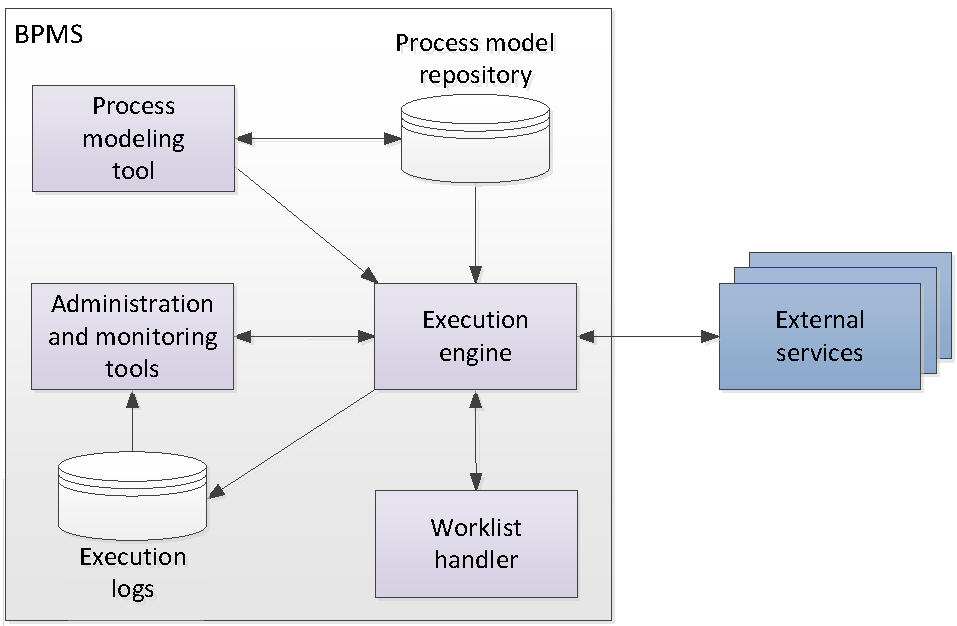
\includegraphics[scale=.65]{figure}
%
% If not, use
%\picplace{5cm}{2cm} % Give the correct figure height and width in cm
%
\caption{Please write your figure caption here}
\label{fig:A1}       % Give a unique label
\end{figure}

% For tables use
%
\begin{table}
\caption{Please write your table caption here}
\label{tab:A1}       % Give a unique label
%
% For LaTeX tables use
%
\begin{tabular}{p{2cm}p{2.4cm}p{2cm}p{4.9cm}}
\hline\noalign{\smallskip}
Classes & Subclass & Length & Action Mechanism  \\
\noalign{\smallskip}\hline\noalign{\smallskip}
Translation & mRNA$^a$  & 22 (19--25) & Translation repression, mRNA cleavage\\
Translation & mRNA cleavage & 21 & mRNA cleavage\\
Translation & mRNA  & 21--22 & mRNA cleavage\\
Translation & mRNA  & 24--26 & Histone and DNA Modification\\
\noalign{\smallskip}\hline\noalign{\smallskip}
\end{tabular}
$^a$ Table foot note (with superscript)
\end{table}
%

\nocite{*}

\bibliographystyle{spmpsci}
\bibliography{bib/bala,bib/biblio}

\backmatter%%%%%%%%%%%%%%%%%%%%%%%%%%%%%%%%%%%%%%%%%%%%%%%%%%%%%%%
%%%%%%%%%%%%%%%%%%%%%%acronym.tex%%%%%%%%%%%%%%%%%%%%%%%%%%%%%%%%%%%%%%%%%
% sample list of acronyms
%
% Use this file as a template for your own input.
%
%%%%%%%%%%%%%%%%%%%%%%%% Springer %%%%%%%%%%%%%%%%%%%%%%%%%%

\Extrachap{Glossary}


Use the template \emph{glossary.tex} together with the Springer document class SVMono (monograph-type books) or SVMult (edited books) to style your glossary\index{glossary} in the Springer layout.


\runinhead{glossary term} Write here the description of the glossary term. Write here the description of the glossary term. Write here the description of the glossary term.

\runinhead{glossary term} Write here the description of the glossary term. Write here the description of the glossary term. Write here the description of the glossary term.

\runinhead{glossary term} Write here the description of the glossary term. Write here the description of the glossary term. Write here the description of the glossary term.

\runinhead{glossary term} Write here the description of the glossary term. Write here the description of the glossary term. Write here the description of the glossary term.

\runinhead{glossary term} Write here the description of the glossary term. Write here the description of the glossary term. Write here the description of the glossary term.
%
\Extrachap{Solutions}

\section*{Problems of Chapter~\ref{intro}}

\begin{sol}{prob1}
The solution\index{problems}\index{solutions} is revealed here.
\end{sol}


\begin{sol}{prob2}
\textbf{Problem Heading}\\
(a) The solution of first part is revealed here.\\
(b) The solution of second part is revealed here.
\end{sol}


\printindex

%%%%%%%%%%%%%%%%%%%%%%%%%%%%%%%%%%%%%%%%%%%%%%%%%%%%%%%%%%%%%%%%%%%%%%

\end{document}





